\documentclass[../main.tex]{subfiles}

\begin{document}

\renewcommand{\labelitemi}{\ding{226}}
\renewcommand{\labelitemii}{\ding{227}}

\part{Heavy neutrino study}

\chapter{HNL search prospects in T2K}
\label{ch:hnl}

As mentioned in the \autoref{ch:intro:HNL} the discovery of the neutrino oscillation phenomena explicitly indicates non-zero neutrino mass. Several theoretical frameworks were developed trying to describe its nature. Most of them predict the existence of the Heavy Neutral Lepton (HNL) --- an electrically neutral particle, that interacts only through the weak interaction. It's sometimes refereed to as a ``heavy neutrino''. Neutrino Minimal Standard Model ($\nu$MSM, \autoref{sec:intro:numsm}) is a minimal extension to the Standard Model. It postulates the existence of 3 HNLs. One of them $N_1$ is pretty light ($M_{N_1}\propto1keV$) and is responsible for the phenomenon of the Dark Matter. It interacts with SM particles extremely weakly. Two other heavy neutrinos ($N_2,\text{ }N_3$) should interact stronger to explain the observed behavior of neutrino oscillations. Their mass can be in a pretty wide range from 100 MeV/$\text{c}^2$ up to 80 GeV/$\text{c}^2$. To be able to generate the baryon asymmetry in the early Universe they should be nearly degenerated $\Delta M_{2,3}\ll M_{2,3}$.

$N_2$ and $N_3$ interact with the SM particles through the mixing with the active neutrino. Thus they can be produced in the meson decays $H\to\ell+N$. The mixing is expected to be quite weak hence large statistics is essential for the search for such a process. Only experiments with very intense meson beams are sensitive enough for the HNL production detection. For example, kaon experiments (E949 in BHL, NA62 in CERN) are using stopped kaons to study their decay. They measure precisely the kaon decay position, all the daughter particles, and their kinematics. These experiments performed a search for the rare kaon decay into the massive neutrino $K\to\ell+N$ among the dominating decay into an active light neutrino $K\to\ell+\nu$. The signal signature is slightly different kinematics of the HNL production comparing to the decay into a light neutrino.

The other class of setups with an extremely intense meson beam are neutrino accelerator experiments. The neutrino beam is produced with the proton accelerator. Protons hit the target, producing mesons. These mesons are focused with the magnetic field to obtain the intense neutrino beam. Some of the mesons can decay into the exotic particle --- heavy neutrino. There are few neutrino beamline facilities in the world: J-PARC in Japan (T2K experiment) and NuMI in the USA (NOvA, MINOS, MINERvA experiments). The meson beam in such experiments is not precisely monitored, so it's not possible to find a rare meson decay with slightly different kinematics, like in the kaon experiments. But there is room for a direct search for the HNL decay. The benefit of the decay search is increased sensitivity for the HNL with high mass. In the kaon experiments, higher mass causes low momentum lepton that is hard to detect. On the contrary, high HNL mass causes more energetic daughter particles and increases the detection efficiency in the decay search experiments.

The most probable HNL decays are $N\to\mu\pi$ and $N\to e\pi$. In the neutrino experiments, we expect a huge amount of similar events from neutrino interactions. Neutrino can interact with the nucleus, producing lepton and pion $\nu_\mu+N\to\mu+\pi+N'$ and $\nu_e+N\to e+\pi+N'$. The huge advantage of the T2K experiment in the search for the HNL is a near detector configuration. As it was widely described in the \autoref{ch:T2K:general} the ND280 detector uses two scintillator targets alternated with three atmospheric pressure TPCs. The gaseous detectors are extremely interesting in the search for the heavy neutrino. The rate of neutrino interactions in gas is extremely low. Even more so the main reaction mode at T2K energies is quasi-elastic interaction, but not the pion production. ND280 is magnetized, so it can separate the oppositely charged lepton and pion from HNL decay. The TPCs provide particle identification with energy loss and also have a good spatial resolution. The latter is essential to select the interactions inside the TPCs only, as we expect many neutrino interactions in the material around the gas volume and the other detectors.

\section{Analysis overview}
In the current work, I study a possibility of the improvement of the constraints on the HNL mixing elements in the T2K experiment. As mentioned above, T2K is expected to have remarkable sensitivity because of the very intense meson beam and the configuration of the near detector. The 30 GeV proton beam from J--PARC accelerator produces mostly pions and kaons. The neutrino and anti-neutrino spectra divided into the parent particle type are presented in \autoref{fig:HNL:meson_flux}.

\begin{figure}[!ht]
    \centering
    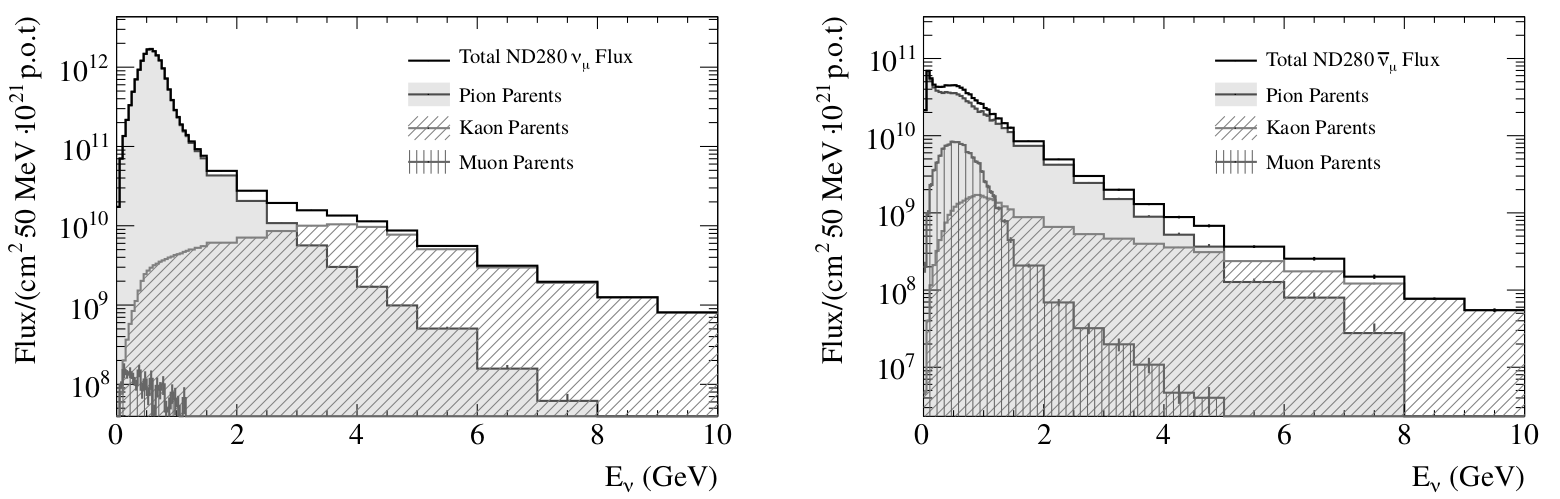
\includegraphics[width=\linewidth]{meson_flux}
    \caption{The muon neutrino and anti-neutrino flux prediction at the ND280 broken down by the neutrino parent particle type.}
    \label{fig:HNL:meson_flux}
\end{figure}

Neutrino from pions are dominating but there is still a notable contribution from the kaon decay. Kaons are much more preferable for heavy neutrino studies as they allow us to study a wider mass range. The various HNL production and decay modes are overviewed in~\cite{Gorbunov2007}. I will use the two-body kaon decay $K\to\ell+N$ as the main source of the potential heavy neutrinos. Three-body reactions are much rarer. Also, they provide less focused HNL beam, thus fewer particles will reach near detector. Among the heavy neutrino decay modes, I will choose the ``visible'' ones that produce charged particles (e.g. $N\to\nu\nu\nu$ mode is omitted). The most probable among them are two-body decays into lepton and pion. Three-body reactions with the neutrino in the final state are less probable, but also considered in the current analysis. The chosen heavy neutrino production and decay modes are presented in \autoref{fig:HNL:mass_scale}. The HNL mass ranges allowed by the kinematics for each particular mode are shown.

\begin{figure}[!ht]
    \centering
    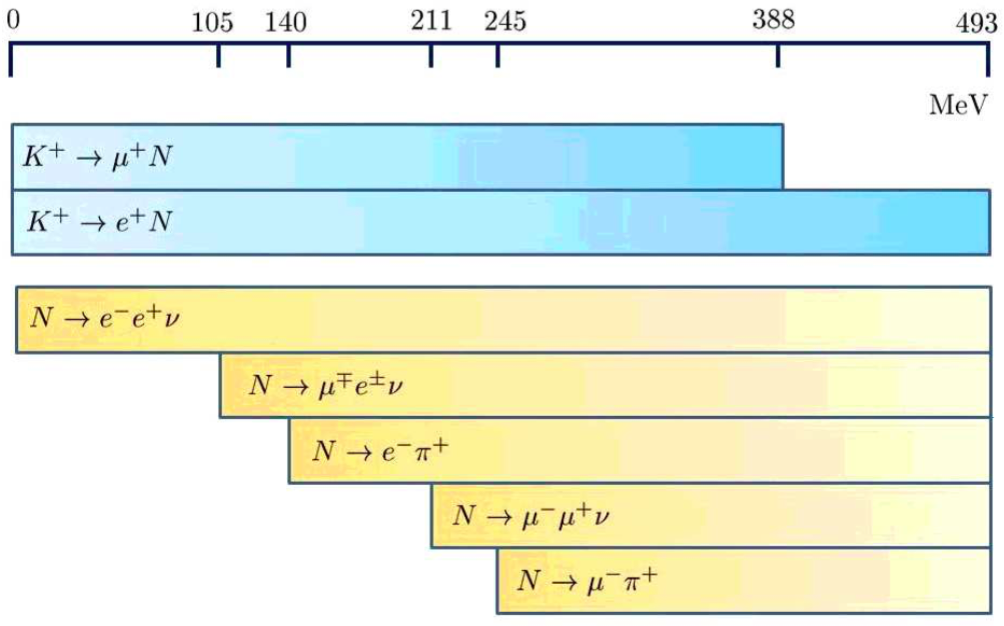
\includegraphics[width=0.7\linewidth]{HNL_mass_scale}
    \caption{Summary of the production and detection processes of the heavy neutrino available for the analysis with the ND280. The horizontal axis corresponds to the HNL mass}
    \label{fig:HNL:mass_scale}
\end{figure}

The three ND280 TPCs will be used as a fiducial volume to search for the HNL decay. The density of the atmospheric pressure gaseous detectors is nearly 3 orders of magnitude smaller comparing to scintillator targets. Thus superior suppression of the active neutrino interactions is reached. The expected event signature is a production of the oppositely charged lepton and pion in the gas. The TPC allows to reconstruct accurately decay vertex position. The ND280 detector will provide the separation of the charged particles in the magnetic field. No activity is expected upstream to the vertex as we are looking for the neutral particle decay. The simulation of the signal events and the detector response as well as detector efficiency will be presented in \autoref{sec:HNL:eff} of \autoref{ch:HNL:ana}.

The most probable background for the process of interest is the active neutrino interactions. Though their rate is quite low in the gas, with the large statistics we will still see some of them. The most dangerous process is pion production as it will mimic the signal. But such a background can be separated from the signal based on the different kinematics. The direction of the heavy neutrino can be reconstructed based on daughter particles tracks and it's expected to be strictly collinear to the neutrino beam. During the active neutrino scattering over the nucleus (e.g. $\nu+n\to\mu+\pi+p$) the direction of the $\mu\pi$ pair can be distributed over a wide angle.

\begin{comment}
It happens because of the nuclear effects such as Fermi motion and secondary interactions in nuclei (\autoref{sec:intro:nuclei} of \autoref{ch:nu_phys}). Thus the background can be further reduced with the kinematics cuts. The detailed analysis of the background will be presented in \autoref{sec:HNL:bg} of \autoref{ch:HNL:ana}.
\end{comment}

We are going to search for the low-rate process in the low background environment. The usual method to compute the upper limit on the process of interest in such a case is Feldman \& Cousins approach~\cite{Cousins1998}. In my analysis proper treatment of the uncertainty is essential. Thus I will use the different algorithm that was developed by Highland \& Cousins~\cite{Cousins1992}. The details about the statistical interpretations of the results will be overviewed in \autoref{sec:HNL:stat} of \autoref{ch:HNL:ana}.

The prediction of the possible improvements on the upper limits of the HNL mixing elements in the T2K experiment was done by Asaka~\cite{Asaka2012}. One of the main goals of my study is to check the phenomenological prediction and to proceed to the final results.


\chapter{HNL signal simulations}
\label{ch:HNL:HNLsim}
The first step of the analysis is the simulation of the HNL flux at the ND280. The simulation of neutrino flux at the near detector has already been developed for the oscillation analysis. I decided to use the obtained results and adapt them to the HNL analysis. With this simulation, we have all the information about the neutrinos entering the ND280 and their parent particles. Because of the kinematics, the phase space of the meson decay into HNL is more limited than the decay into a nearly massless neutrino. E.g. the maximum angle of the HNL direction with respect to the parent meson direction is lower comparing to the massless neutrino case. Thus if we consider only mesons that can produce neutrino entering ND280 and omit all the others, we will definitely take all the possible HNL parent particles.

For the heavy neutrino simulation, we consider the particular meson decay and reweight it taking into account new kinematic and the branching ratios. Thus we will obtain the heavy neutrino spectrum in our detector. The next step is the simulation of the HNL decay in the sensitive detector. I considered two- and tree-body decays of the heavy neutrino. A random direction of the daughter particle was generated and the appropriate decay width was taken into account. Thus I obtained the Monte--Carlo signal samples that can be used for the selection optimization and the detector systematic studies.

\section{T2K flux simulation}
The accurate prediction of the neutrino flux is extremely important for precise oscillation analysis. That's why the T2K collaboration has spent great effort into tuning the flux simulation most accurately~\cite{Abe2013}. All the elements of the neutrino beamline are taken into account. The most tricky part is the evaluation of meson production through the proton interactions in the carbon target. As this step is critical for the HNL study, I will overview the simulation process in detail.

The overview of the T2K beamline is presented in \autoref{ch:T2K:nu_beam} of \autoref{ch:T2K:general}. The proton beam spatial distribution and divergence are measured with the beamline monitors. The FLUKA generator is used to perform the simulation of the hadron interaction with the target and a baffle. The position and direction of an incident proton is well--defined with beamline monitors measurements. Proton energy is set to 30 GeV. The information of the generated particles that exited the target volume is stored. The cross--section and the multiplicity of the meson production is a subject of uncertainty. The NA61/SHINE experiment has performed the series of measurements with the T2K-replica target to measure precisely the process of interest.

\begin{bclogo}[couleur=blue!2, arrondi=0.1, logo=\bcinfo, nobreak=true]{NA61/SHINE experiment}
The NA61/SHINE (SPS Heavy Ion and Neutrino Experiment)~\cite{Abgrall2014} is a multi-purpose facility at CERN that operates with a secondary beam from the Super Proton Synchrotron (SPS) in the North Area of CERN. A 450 GeV proton beam is focused on the primary target. The secondary particles with given momentum are selected by the horn system and focused on the secondary target. The main physics goals are:
\begin{itemize}
    \item study the properties of the onset of QCD deconfinement and search for the quark--gluon plasma critical point with investigating p+p, p+Pb and nucleus-nucleus collisions,
    \item precise hadron production measurements for improving calculations of the initial neutrino beam flux in the long-baseline neutrino oscillation experiments as well as for more reliable simulations of cosmic-ray air showers.
\end{itemize}

The detector operates at the fixed target made from different materials (carbon, beryllium, etc.). The detector scheme is presented in \autoref{fig:HNL:NA61}. The setup consists of the trigger system, TPC tracking system with superconducting magnets, time of flight detectors and Projectile Spectator Detector (PSD).

For the T2K purpose the experiment performed the measurements of the hadron interaction multiplicities with a proton beam and a carbon T2K-replica target. The beam with T2K energies and an exact replica of the T2K target was used. This data allows to constrain the neutrino production at the T2K much more precisely.
\end{bclogo}

\begin{figure}[!ht]
    \centering
    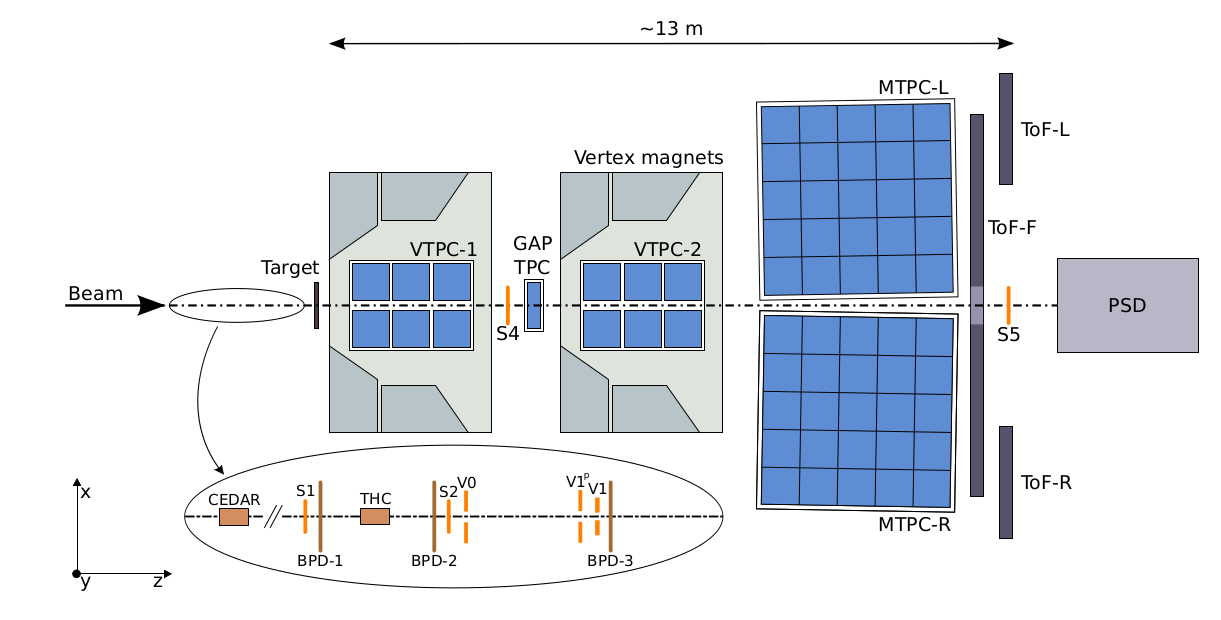
\includegraphics[width=\linewidth]{NA61.png}
    \caption{The scheme of the NA61/SHINE experiment.}
    \label{fig:HNL:NA61}
\end{figure}

\begin{figure}[!ht]
    \centering
    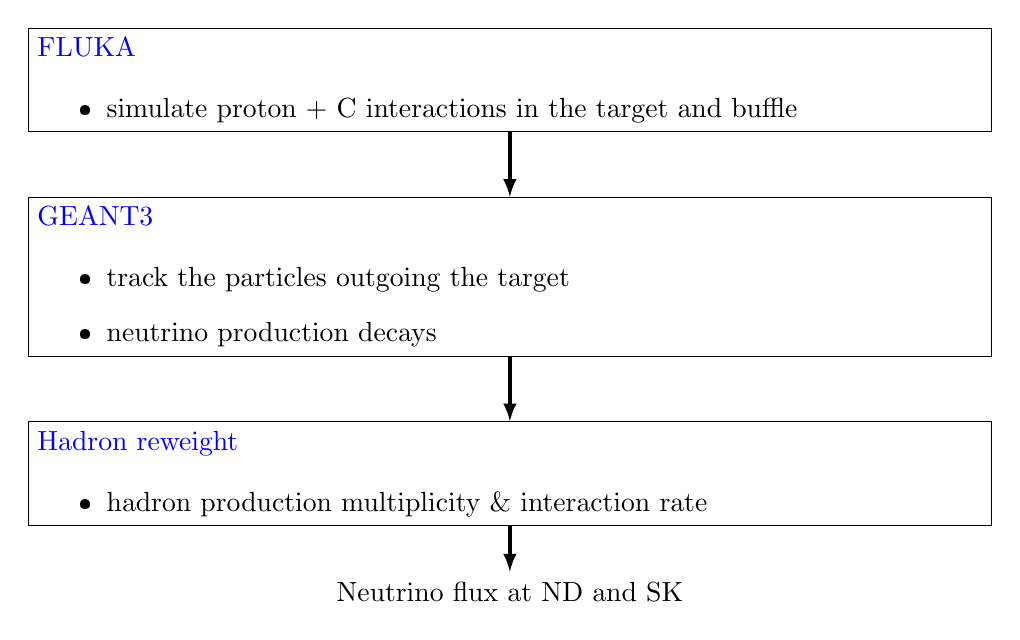
\begin{tikzpicture}
    \tikzstyle{noeud}=[align=left,text width=12cm, minimum height=0.5cm, rectangle,draw]
    \tikzstyle{noeuu}=[align=center,text width=12cm, minimum height=0.5cm]
    \node[noeud] (N01) at (0, 2.5) {\textcolor{blue}{FLUKA} \\  \begin{itemize} \item simulate proton + C interactions in the target and buffle \end{itemize}};
    \node[noeud] (N02) at (0, 0) {\textcolor{blue}{GEANT3} \\  \begin{itemize} \item track the particles outgoing the target \\ \item neutrino production decays \end{itemize}};
    \node[noeud] (N03) at (0, -2.5) {\textcolor{blue}{Hadron reweight} \\ \begin{itemize} \item hadron production multiplicity \& interaction rate\end{itemize}};
    \node[noeuu] (N04) at (0, -4) {Neutrino flux at ND and SK};

    \tikzstyle{link}=[->,very thick,>=latex]
    \draw[link] (N01) -- (N02);
    \draw[link] (N02) -- (N03);
    \draw[link] (N03) -- (N04);
    \end{tikzpicture}

    \caption{The neutrino flux prediction flow}
    \label{fig:HNL:nu_flux_sim}
\end{figure}

The flow diagram of the neutrino flux simulation is shown in \autoref{fig:HNL:nu_flux_sim}. After the meson production simulation, we track them through the horns, helium vessel, decay volume, and surrounding concrete until the decay or the kinetic energy drop down below the threshold (10 MeV). The GEANT3 simulation toolkit is used for this purpose. At this step $\pi^\pm$, $K^\pm$, $K_L^0$, and $\mu^\pm$ decays are considered as neutrino sources. To save computing time, the daughter neutrino is pointing towards the Super--Kamiokande and the appropriate kinematic weight is assigned to the event.

After such a simulation chain is performed and the outgoing neutrino is registered the hadronic chain in each event is re-weighted based on the hadron interaction measurements. In our studies, we are particularly interested in kaon production. The generated kaon phase space and the coverage of the NA61 measurements are presented in \autoref{fig:HNL:kaon_ps}.

After the reweighting of the hadron chains, the total accuracy of the prediction is evaluated~\cite{Abe2013}. The main systematic errors come from the hadronic interactions, primary beam alignment, horn current, and magnetic field. The resulting uncertainty of the neutrino flux predictions is shown in \autoref{fig:HNL:nu_flux_uncert}.

\begin{figure}[!ht]
    \begin{minipage}[!ht]{0.49\linewidth}
        \centering
        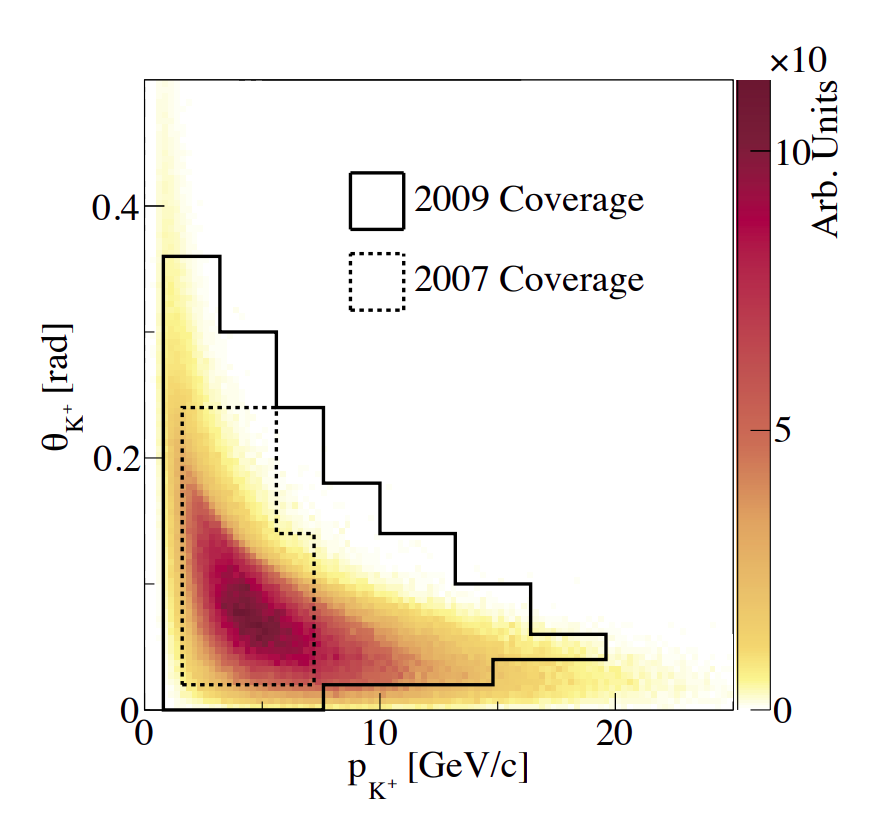
\includegraphics[width=\linewidth]{nu_flux_kaons}
        \caption{The phase space of positive kaons contributing to the predicted neutrino flux and the regions covered by the NA61/SHINE.}
        \label{fig:HNL:kaon_ps}
    \end{minipage}
    \hfill
    \begin{minipage}[!ht]{0.49\linewidth}
        \centering
        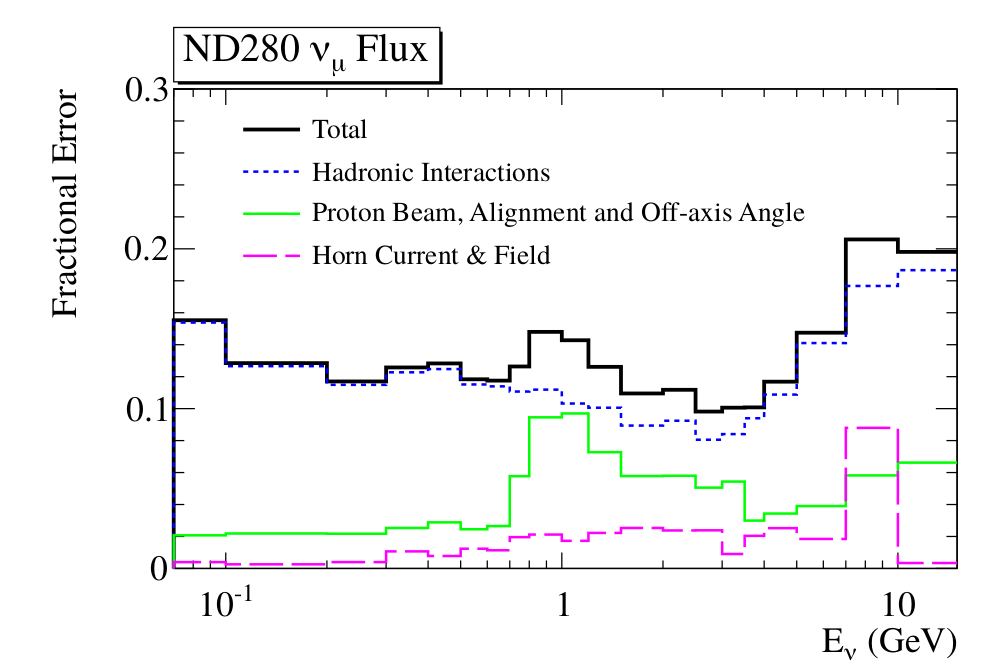
\includegraphics[width=\linewidth]{nu_flux_uncert}
        \caption{Fractional errors for the muon neutrino flux.}
        \label{fig:HNL:nu_flux_uncert}
    \end{minipage}
\end{figure}


\section{HNL production}
For the purpose of our study, I would like to reweight the kaon decays for the case of HNL production. But I want to use all the fine-tuning described in the previous section to keep the uncertainties as small as possible. Looking at the \autoref{fig:HNL:nu_flux_sim}, I would like to apply a new weight at the second step ``neutrino-producing decays'', but to keep everything else at place. The HNL production will be different from the decay into active neutrino because of the different branching ratios and the kinematic weight.

The new branching ratio is calculated according to~\cite{Gorbunov2007}:
\begin{equation}
    \begin{split}
    Br(K\rightarrow \ell+N)&=\frac{G_F^2 V_{us}^2 f_K^2 M_K M_{HNL}^2}{8\pi\hbar}\left(1-\frac{M_{HNL}^2}{M_K^2}+\frac{2M_\ell ^2}{M_K^2}+\frac{M_\ell^2}{M_{HNL}^2}\left(1-\frac{M_\ell^2}{M_K^2}\right)\right) \\
&\sqrt{\left(1+\frac{M_{HNL}^2}{M_K^2}-\frac{M_\ell^2}{M_K^2}\right)^2-\frac{4M_{HNL}^2}{M_K^2}} \cdot\tau_K,
    \end{split}
    \label{eq:HNL:Kdecay}
\end{equation}
where
\begin{itemize}
\item $G_F$ --- Fermi constant,
\item $V_{us}$ --- the CKM matrix element,
\item $M_\ell$ and $M_{HNL}$ --- the lepton and the HNL masses,
\item $M_K, f_K, \tau_K$ --- kaon mass, form-factor, lifetime respectively.
\end{itemize}

The usual approach for the decay simulation is to throw the daughter particle direction uniformly in $4\pi$ angle. But in this case, most of the particles are lost because they will not rich the detector. To gain the simulation statistics I pointed all the produced heavy neutrinos into ND280. But to keep the total number of events consistent I assigned a weight to each heavy neutrino. The geometry weight is calculated as a probability of a daughter particle to have a momentum with a certain angle $\theta$ w.r.t. the parent momentum. As kaons mostly decay in flight I also need to apply the Lorentz boost from the center of mass frame to the laboratory frame.

\begin{align}
    weight_{geom, lab}&=\frac{p_{lab}E_{cm}}{p_{cm}^2}\cdot weight_{geom,cm}
    \nonumber \\
    weight_{geom, cm} &= \frac{1}{4\pi}\delta\left(p-p_{cm}\right)
\end{align}
The final expression for the geometry weight will look like
\begin{equation}
    weight_{geom, lab}=\frac{1}{4\pi}\frac{p_{lab}E_{cm}}{p_{cm}^2}\frac{cos\theta_{lab}\left(\beta/\beta_{lab}\pm\sqrt{1+\gamma^2\left(1-\left(\beta/\beta_{lab}\right)^2\right)tg^2\theta_{lab}}\right)}{\gamma\left(1-\beta^{2}cos^{2}\theta_{lab}\right)}.
    \label{eq:HNL:lorentz}
\end{equation}

Here I assume that the HNL's lifetime is large enough to reach the ND280. From the cosmology~\cite{Gorbunov2007} we have an upper bound on the HNL lifetime  $\tau < 0.1s$, which is mainly based on the baryogenesis models. So for the current analysis I have the HNL lifetime region $1\mu s\ll\tau<0.1s$ which is wide enough. An estimation of the corresponding mean free path of the HNL gives $\Lambda_{HNL}=c\beta\gamma\tau\gg280 m$.

To cross-check my kinematic model I compared the HNL spectra for $M_{HNL}=0$ with the active neutrino spectrum from $K\mu2$ and made sure that they are identical. After performing modeling of all kaon decays I got the HNL spectra at the ND280 entrance plane (\autoref{fig:HNL:fluxKpos}).

\begin{figure}[!ht]
    \begin{minipage}{0.49\linewidth}
        \center{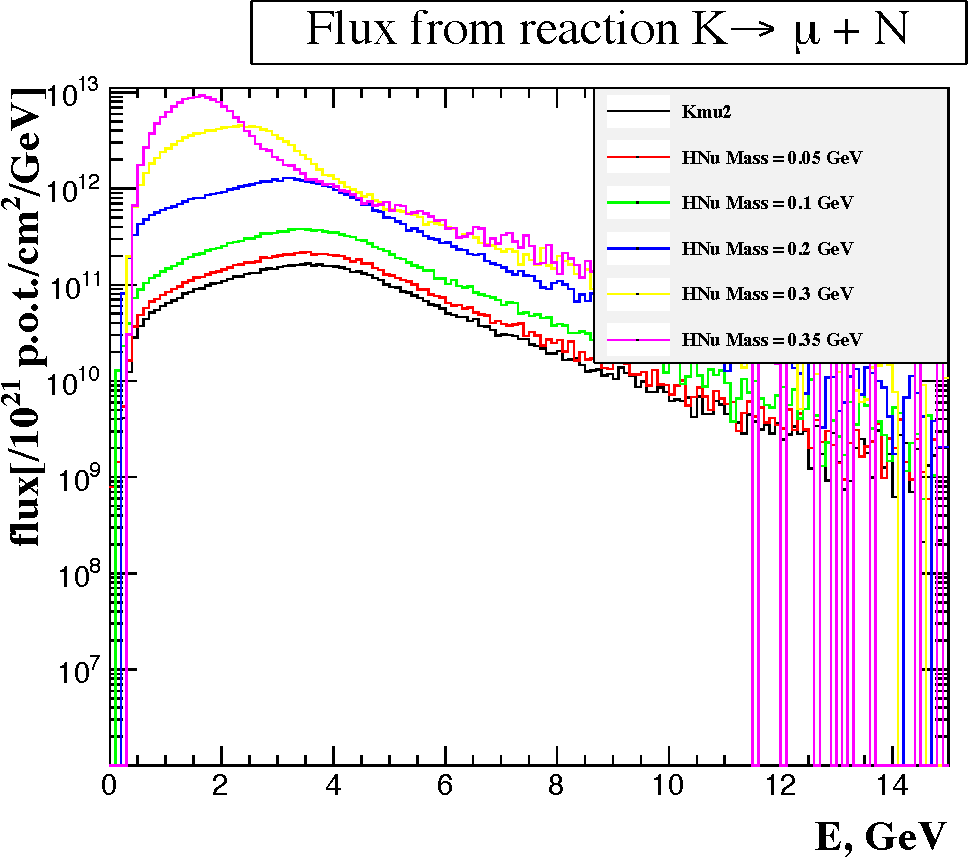
\includegraphics[width=\linewidth]{fluxKmu} \\ $K^+\rightarrow \mu^+N$}
    \end{minipage}
    \hfill
    \begin{minipage}{0.49\linewidth}
        \center{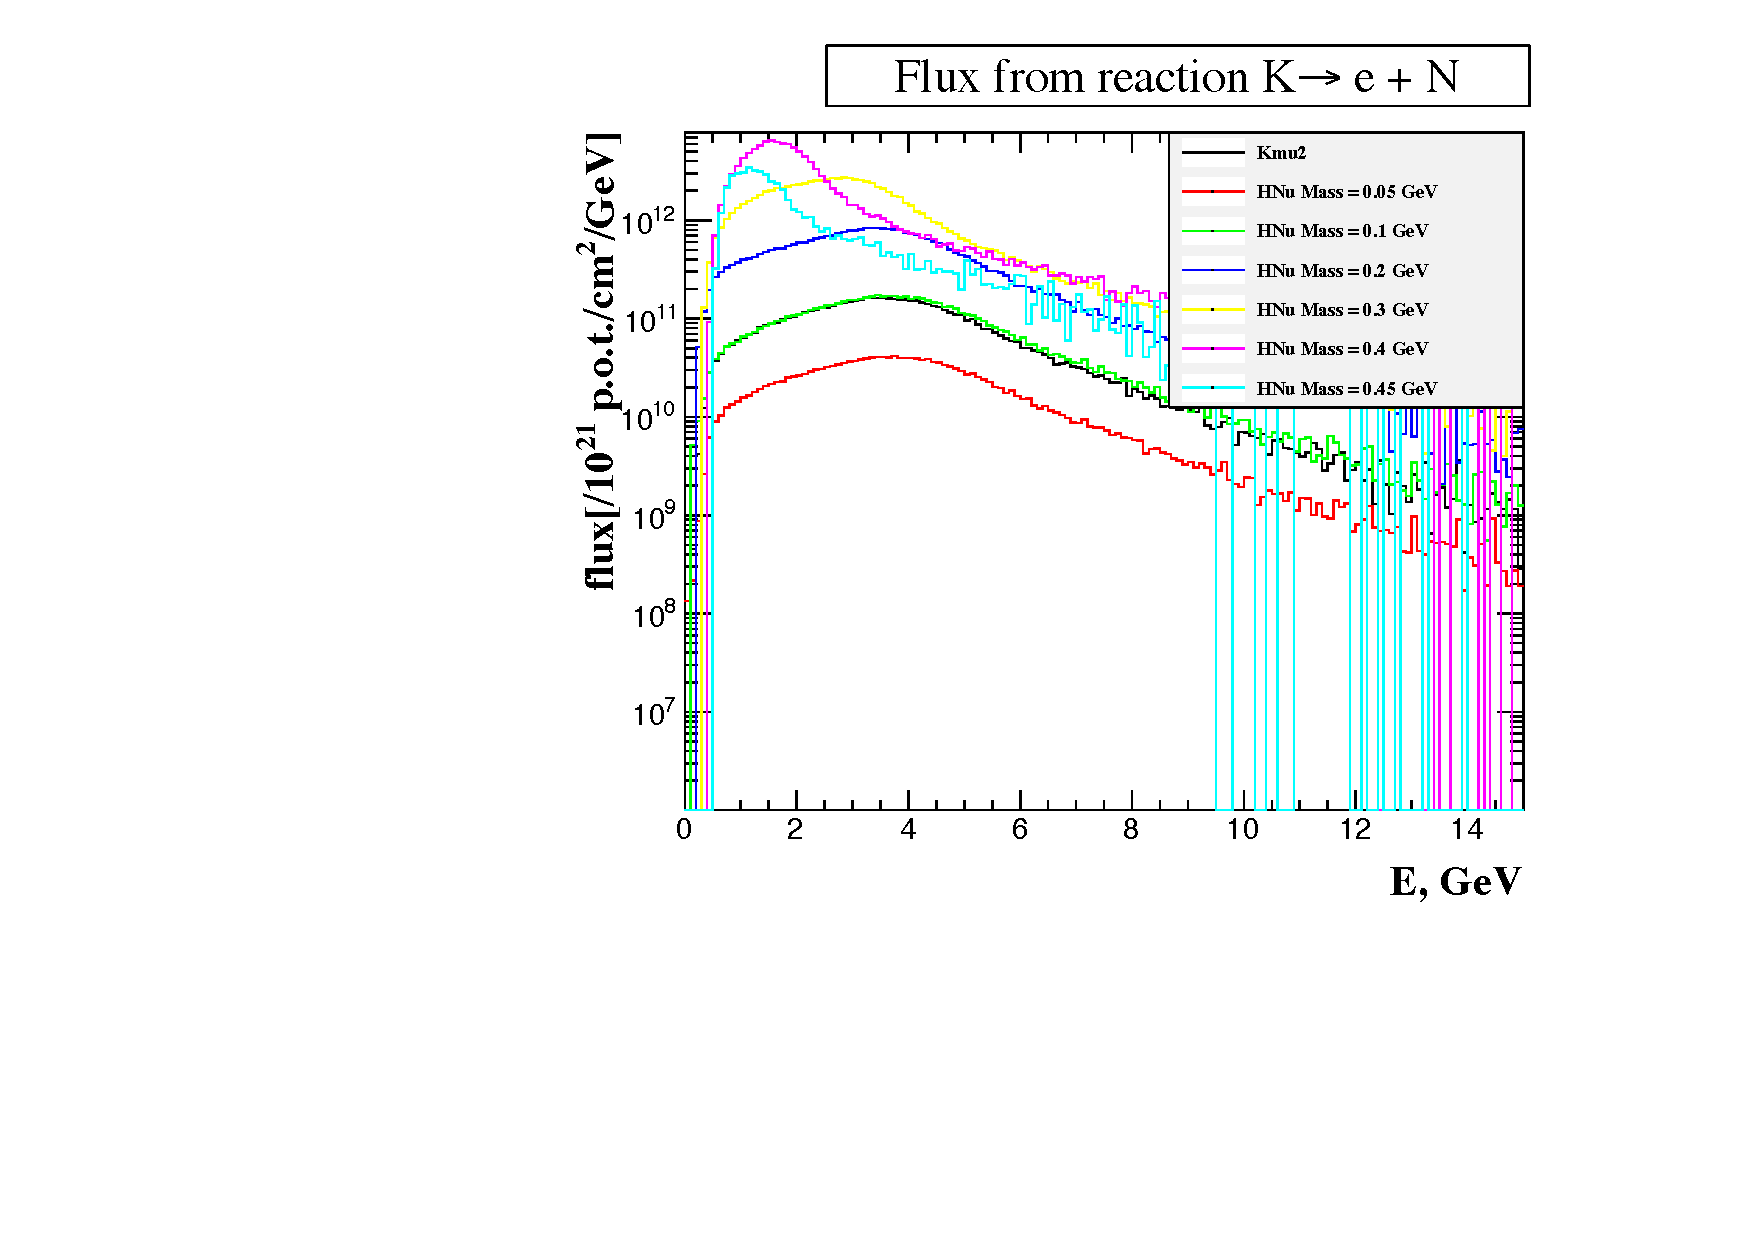
\includegraphics[width=\linewidth]{fluxKe} \\ $K^+\rightarrow e^+N$}
    \end{minipage}
    \caption{HNL energy spectra at the ND280 front plane for two production modes: $K^+\rightarrow \mu^+N$ and $K^+\rightarrow e^+N$ for the different HNL masses.}
    \label{fig:HNL:fluxKpos}
\end{figure}

There are two effects, that cause the flux difference comparing to the active neutrino flux. The first one is the ``massive'' kinematic of the parent meson decay. This correction is calculated according to \autoref{eq:HNL:lorentz}. This impact is shown in \autoref{fig:HNL:fluxMassKpos}. The branching ratio is assumed equal to 1. One can see that the higher mass increases the probability of the HNL to reach the detector. It's understandable as with the higher mass the maximum heavy neutrino angle w.r.t. kaon direction becomes lower. Most of the kaons decay in flight and the HNL is boosted towards the near detector.

\begin{figure}[!ht]
    \begin{minipage}{0.49\linewidth}
        \center{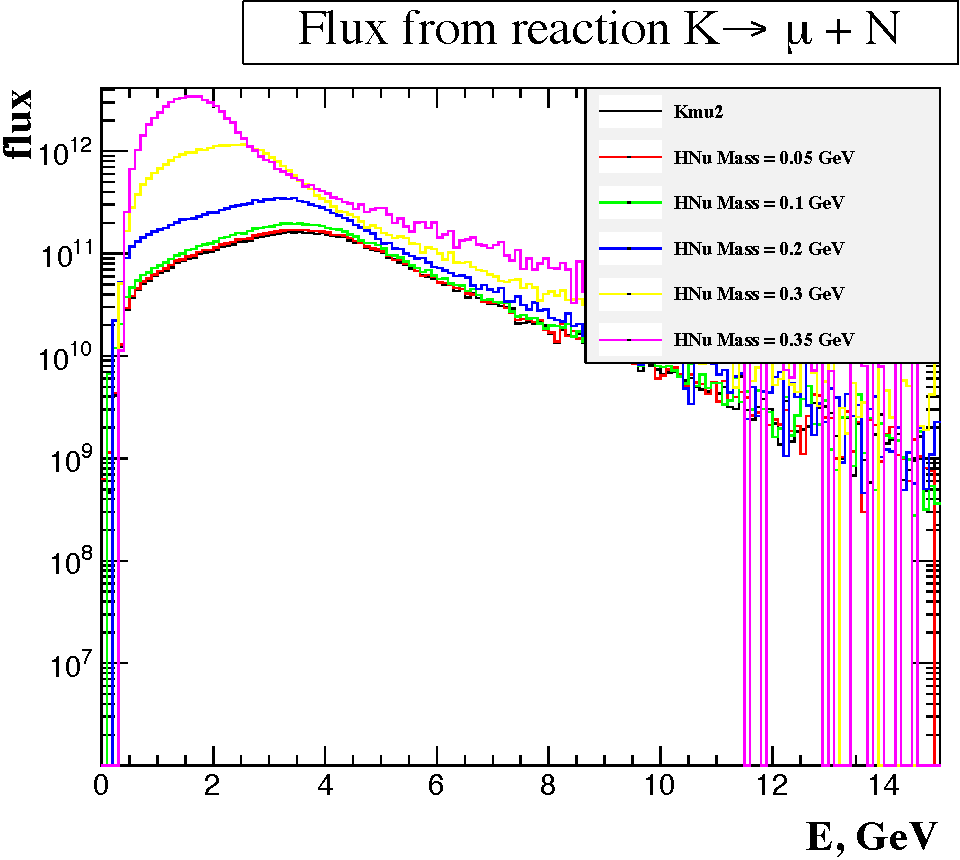
\includegraphics[width=\linewidth]{fluxMassKmu} \\ $K^+\rightarrow \mu^+N$}
    \end{minipage}
    \hfill
    \begin{minipage}{0.49\linewidth}
        \center{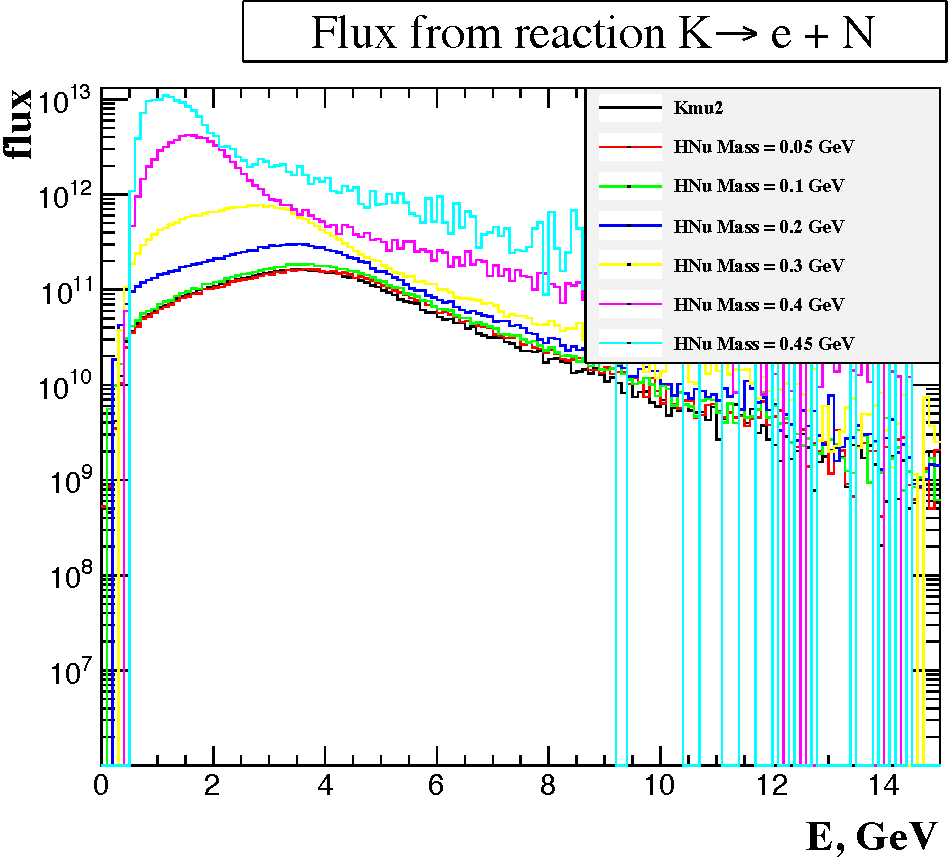
\includegraphics[width=\linewidth]{fluxMassKe} \\ $K^+\rightarrow e^+N$}
    \end{minipage}
    \caption{HNL spectra at the ND280 front plane for two modes and for the different HNL masses assuming the branching ratios equal to 1.}
    \label{fig:HNL:fluxMassKpos}
\end{figure}

The second effect is the modification of the branching ratio of the kaon decay. It is calculated according to \autoref{eq:HNL:Kdecay}. The branching ratio dependence is shown in \autoref{fig:HNL:KdecayBR}. Notice that it can be larger than 1 as the mixing element is considered 1, in reality, it will reduce the branching ratio below the level of one. The branching ration is decreasing dramatically for the low and high regions of the HNL mass. Sometimes low branching ratio can cancel the benefits from the kinematics. E.g. the light HNL flux from the $K\to e+N$ decay is lower than the active neutrino flux from $K\mu2$.

\begin{figure}[!ht]
    \begin{minipage}[!ht]{0.49\linewidth}
        \center{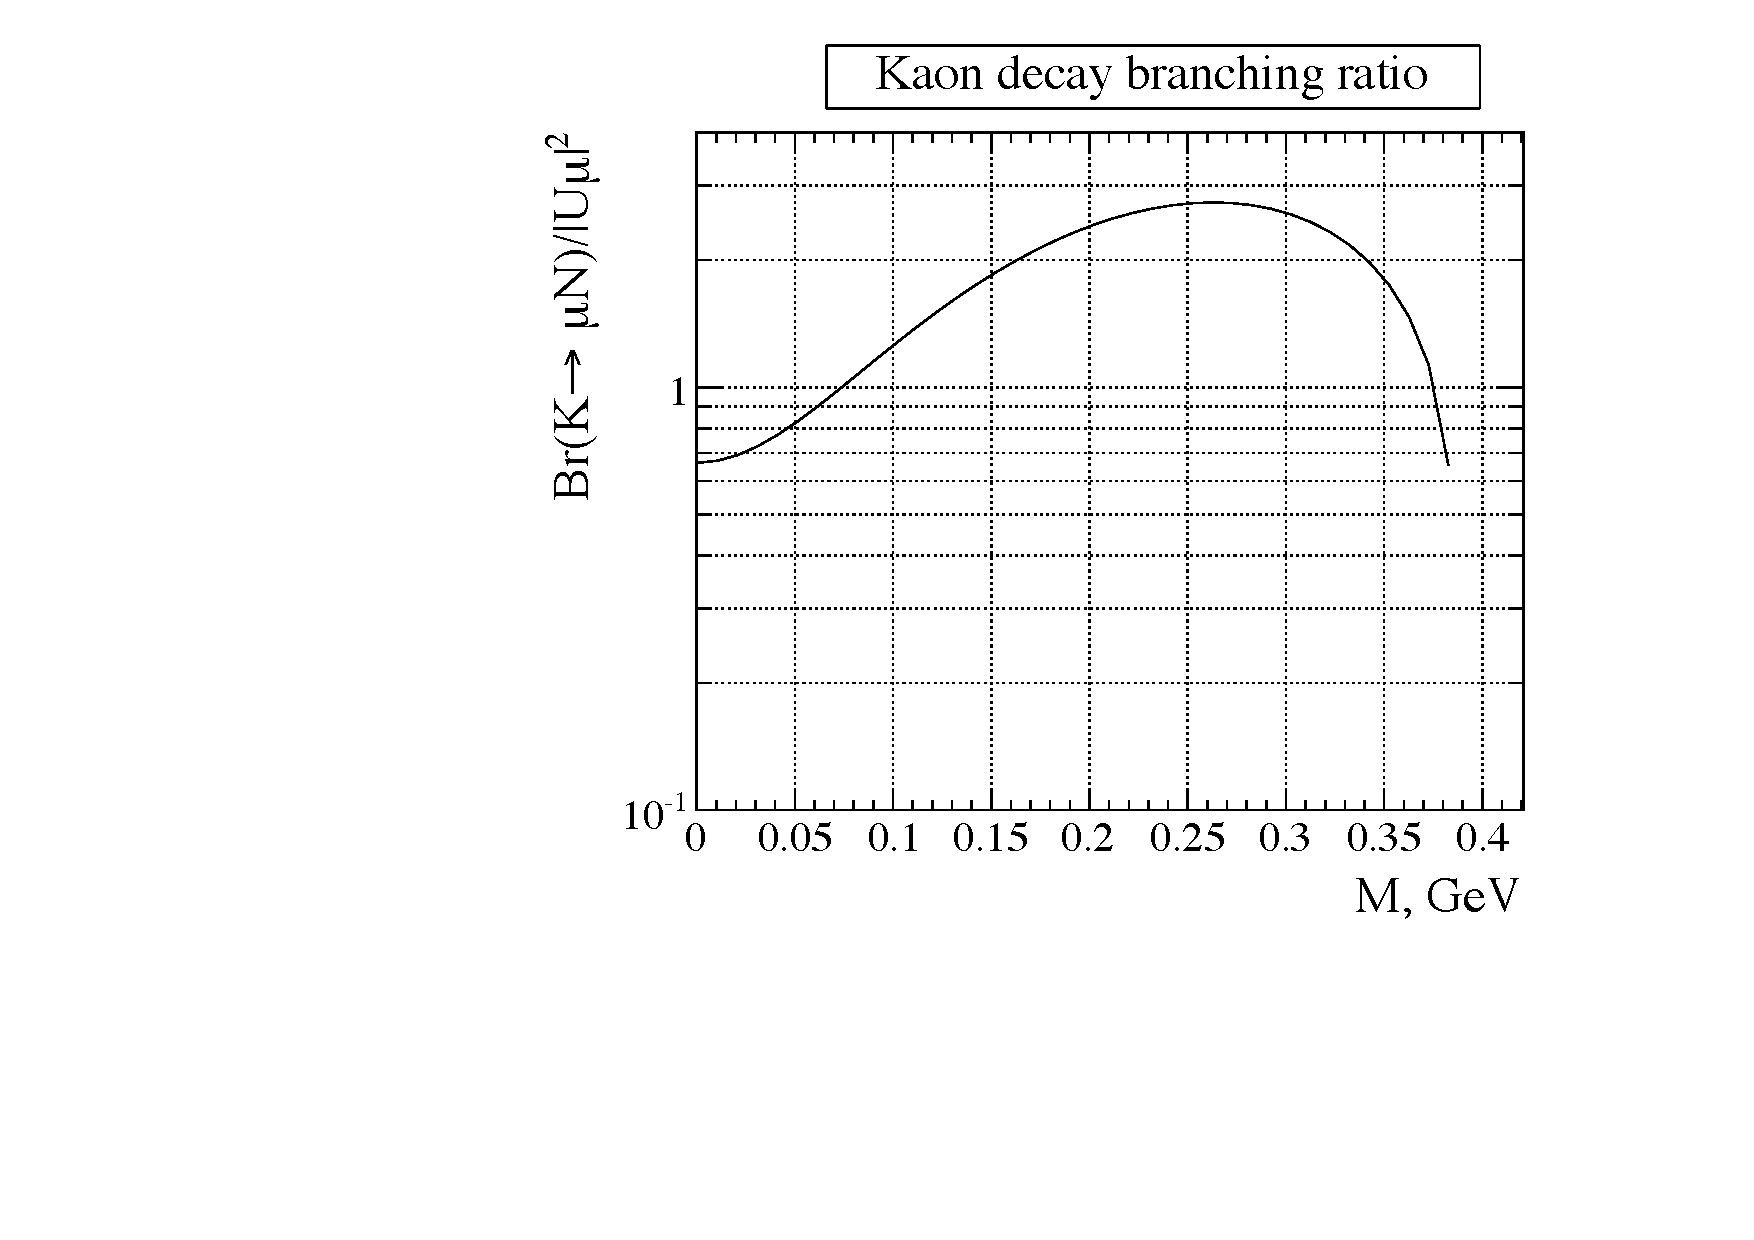
\includegraphics[width=\linewidth]{BrKMu} \\ a)}
    \end{minipage}
    \hfill
    \begin{minipage}[!ht]{0.49\linewidth}
        \center{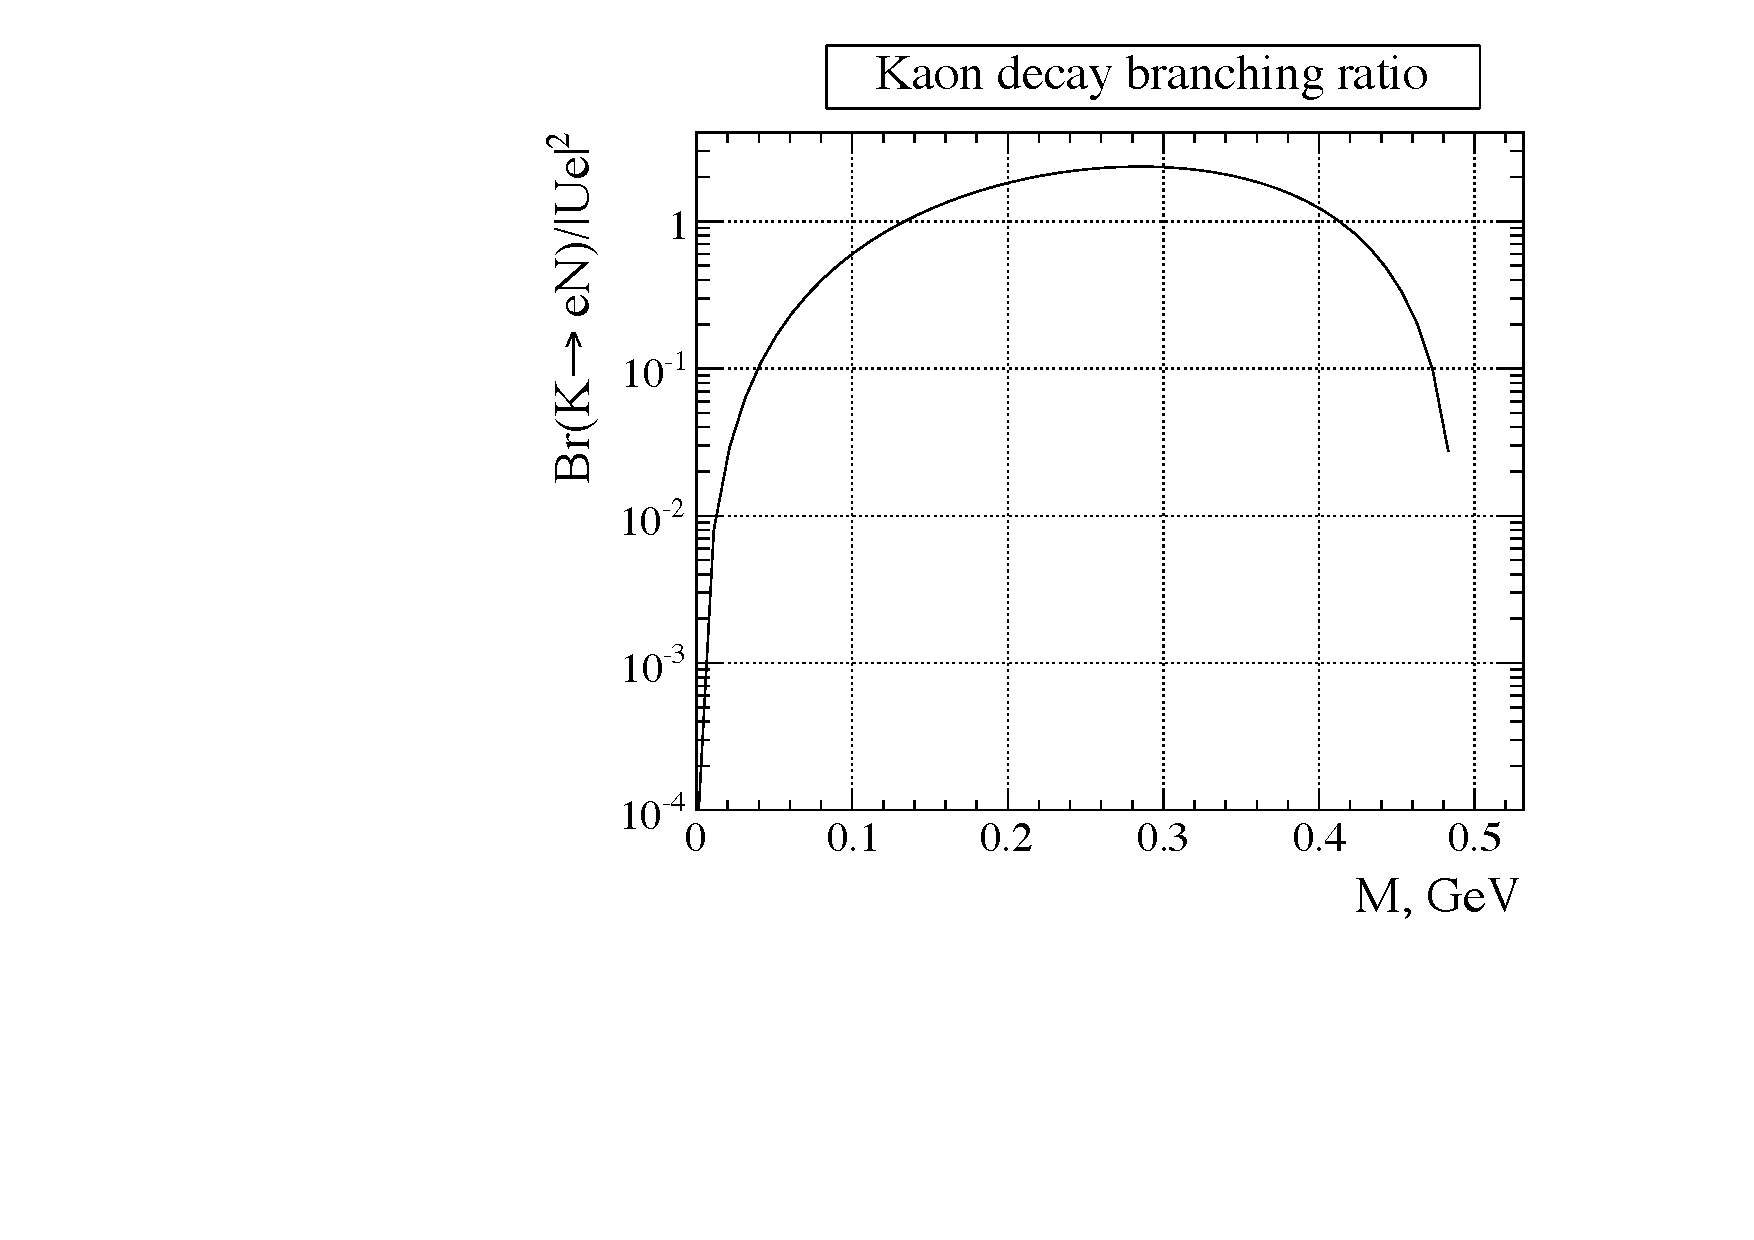
\includegraphics[width=\linewidth]{BrKEle} \\ b)}
    \end{minipage}
    \caption{Kaon decay branching ratio divided into the mixing element for two modes: (a) $K\to \mu N$ and (b) $K\to eN$.}
    \label{fig:HNL:KdecayBR}
\end{figure}

In our study, I assume the Majorana nature of the HNL. Hence the parent meson charge is irrelevant. In the analysis, I combine the heavy neutrinos from both $K^+$ and $K^-$ decays. As one can see in \autoref{fig:HNL:meson_flux} the neutrino flux from the $K^-$ is nearly 3 times smaller comparing to one from $K^+$. It is caused by the lower negative kaon production cross--section.

\section{HNL decays}
Now I have all the information about the HNLs that enter ND280. Thus I can generate the secondary particles that will be produced in the heavy neutrino decay. It will be the expected signal in my analysis. The decay itself is simulated in the HNL rest frame. Then the boost is applied towards the heavy neutrino initial direction. The decay points are randomly generated along the  HNL tracks inside the TPC volume. So the decay positions are expected to be uniformly distributed in this volume (\autoref{fig:HNL:decayPos}).

The simulation of the 2-body decay is straightforward. The direction of the first particle is thrown isotropically. Then based on both momentum and energy conservation laws the whole decay is parametrized in the HNL rest frame. I will obtain the final kinematics of the daughters with the boost along with the heavy neutrino momentum. The kinematic evaluation is covered in~\cite{Landau2013}, chapter 2.

The 3-body decay case is a bit more complicated. For this mode, I can't just throw all the directions as I have one degree of freedom in the decay. To deal with it I used the normalization with the maximum width of the decay. For each event the following weight is assigned:

\begin{equation}
    weight_{3-body}=weight_{K\rightarrow \ell N}\cdot\cfrac{\cfrac{d\Gamma(p_1,p_2)}{dp_1dp_2}}{max\left(\cfrac{d\Gamma(p_1,p_2)}{dp_1dp_2}\right)}\cdot P,
\end{equation}
where $P$ is a 3-body decay weight from the kinematics. As $weight_{3-body} \le 1$ the total number of 3--body decays is reduced. So this number can not be used for the proper estimation of the total number of events. It is crucial to evaluate the probability of the particular event. Because of the kinematics one event can be easier to reconstruct because of the hardware setup (e.g. larger opening angle), but it can be less probable. As I use these samples for the relative efficiency calculation only, the global normalization can be biased but the relative weight should be treated properly.

\begin{figure}[!ht]
    \center{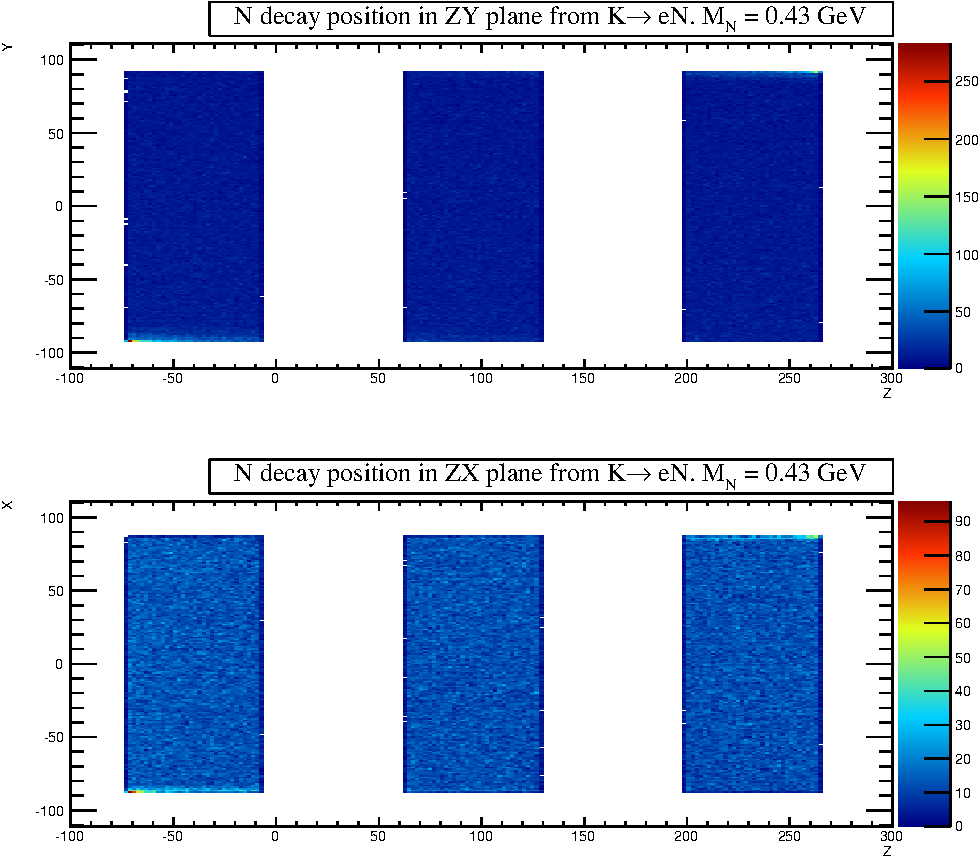
\includegraphics[width=0.7\linewidth]{DecayPos}}
    \caption{Distribution of HNL decay positions over 3 TPCs. The decay position is in the detector coordinate system in mm.}
    \label{fig:HNL:decayPos}
\end{figure}

The polarization of the HNL is taken into account in the simulation according to the calculations from~\cite{Levy2018}. The HNL polarization is given by:
\begin{equation}
    \overrightarrow\prod=\frac{\left(\delta_\ell-\delta_{N}\right)\lambda^{1/2}\left(1,\delta_\ell, \delta_{N}\right)}{\delta_\ell+\delta_{N}-\left(\delta_{N}-\delta_\ell\right)^2}\overrightarrow{n}
\end{equation}
where
\begin{itemize}
    \item $\delta_{N}=\left(M_{N}/m_K\right)^2$
    \item $\delta_\ell=\left(m_\ell/m_K\right)^2$
    \item $\lambda\left(x, y, z\right)=x^2+y^2+z^2-\left(xy+yz+xz\right)$
    \item $\overrightarrow{n}$ is the kaon direction in the heavy neutrino rest frame
\end{itemize}

The polarization of the HNL as a function of its mass in the decay $K\to\mu+N$ is shown in \autoref{fig:HNL:pol}. One can see that in the limit $M_N\to0$ the heavy neutrino behaves exactly as a massless neutrino and becomes left-handed. Also, it's interesting to see that the polarization vanishes when the HNL mass is equal to the muon one.

\begin{figure}[!ht]
    \centering
    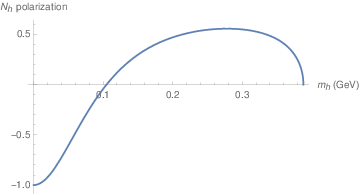
\includegraphics[width=0.5\linewidth]{HNL_pol.png}
    \caption{The polarization of the HNL as a function of its mass in the decay $K\to\mu+N$~\cite{Levy2018}.}
    \label{fig:HNL:pol}
\end{figure}

The polarization of the beam ($\overrightarrow{\prod}$) is a statistical effect. As the HNL is a fermion it can take only discrete polarization: -1 or 1. In the simulation, the polarization value is computed for each decay and a random value is thrown in the range (-1; 1) to determine if the HNL is left-handed or right-handed. Then this characteristic is taken into account during the heavy neutrino decay simulation with:

\begin{equation}
    \frac{dN}{d\cos\theta}\left(N\to\ell\pi\right)\propto\left(1-\delta_\ell'\right)^2-\delta_\pi'\left(1+\delta_\ell'\right)-\frac{\sqrt{\lambda'}}{2}\left(1-\delta_\ell'\right)\prod\cos\theta
\end{equation}

where:
\begin{itemize}
    \item $\delta_\ell'=\left(m_\ell/M_N\right)^2$
    \item $\delta_\pi=\left(m_\pi/M_N\right)^2$
    \item $\lambda'=\lambda\left(1, \delta_\ell', delta_\pi'\right)$
    \item $\theta$ is an angle between the outgoing lepton and the parent meson (kaon) in the HNL rest frame
\end{itemize}


After simulation of the HNL decays I have all information about the kinematics of the daughter particles, i.e. momentum, direction, opening angles. These characteristics are presented in \autoref{fig:HNL:secondary}. It's important to note that most of the particles have momentum below 2 GeV/c. Our TPCs were designed to reconstruct the tracks with momentum below 10 GeV/c. So the charge and the momentum can be precisely measured.

\begin{figure}[!ht]
    \begin{minipage}{0.49\linewidth}
        \centering
        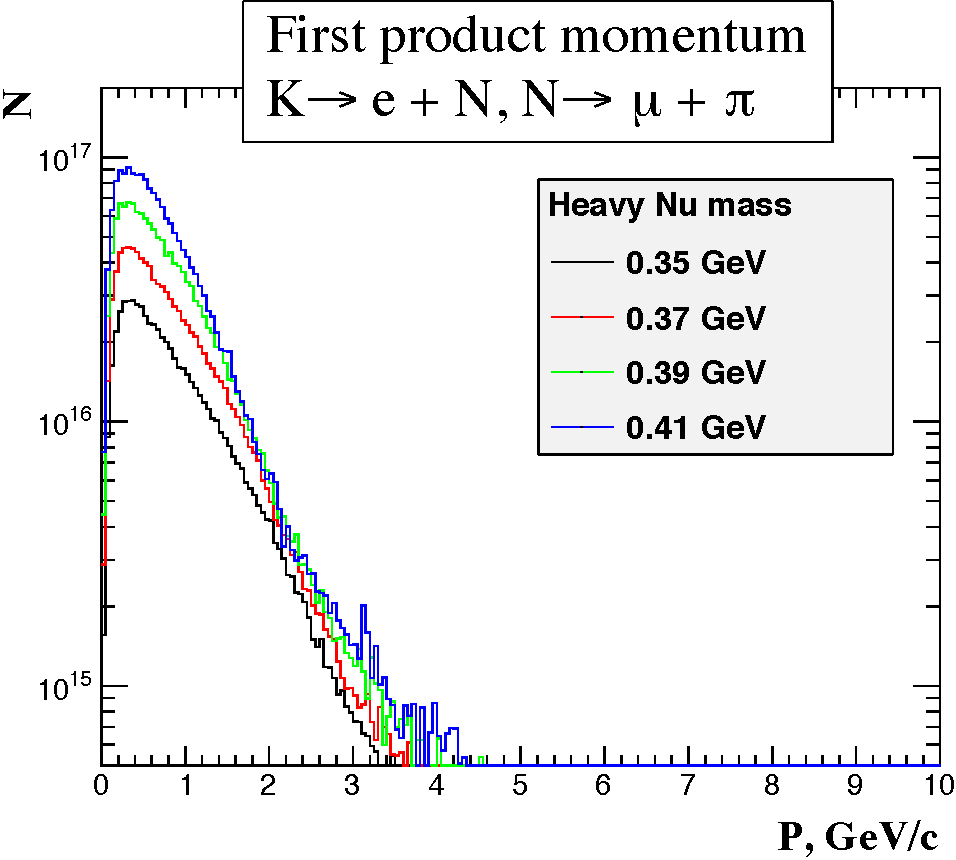
\includegraphics[width=0.8\linewidth]{SecMom} \\ {a}
    \end{minipage}
    \begin{minipage}{0.49\linewidth}
    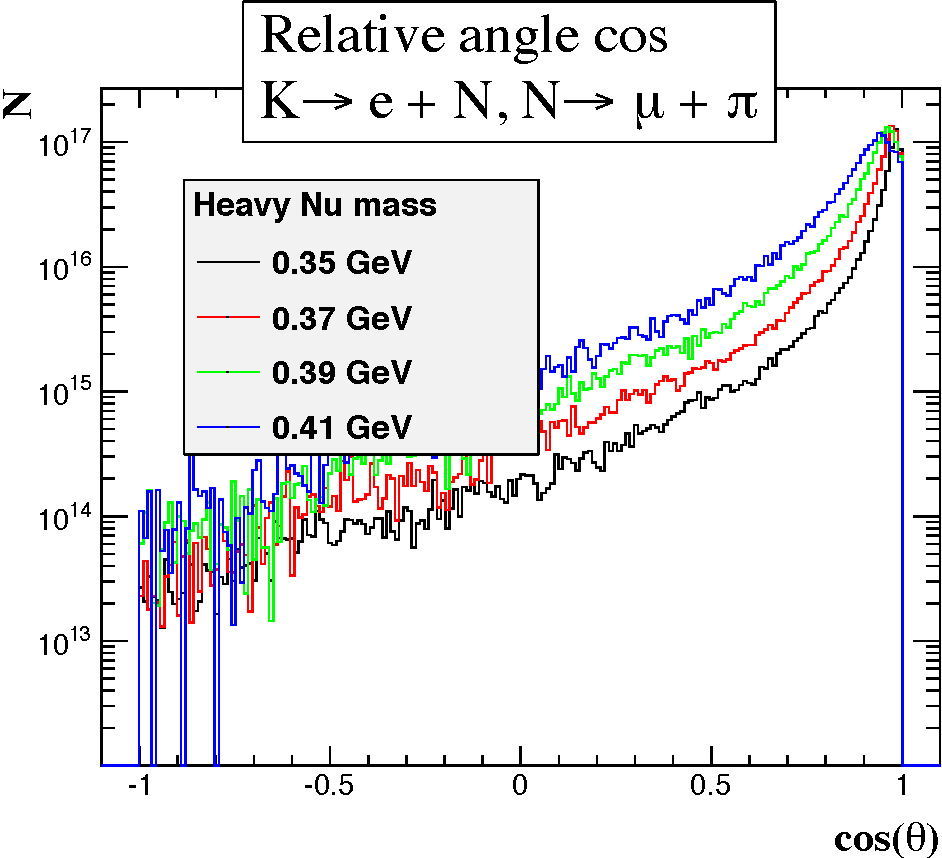
\includegraphics[width=0.8\linewidth]{SecRel} \\ (b)

    \end{minipage}
        \caption{Kinematics spectra of the HNL daughter particles: (a) momentum and (b) opening angle.}
    \label{fig:HNL:secondary}
\end{figure}

The heavy neutrino daughter particles are propagated through the detector with the help of the Geant4 toolkit~\cite{Agostinelli2003}. All the secondary interactions, decays, etc. are considered. An example of a ``good'' MC event with the HNL decay in the first TPC and further evolution of a daughter muon and a pion is shown in \autoref{fig:HNL:event}. The detector response is fully simulated from the initial ionization until the readout signal from the electronics. Thus I can develop the event selection and estimate its efficiency with the MC generated signal sample.
\begin{figure}[!ht]
   \center{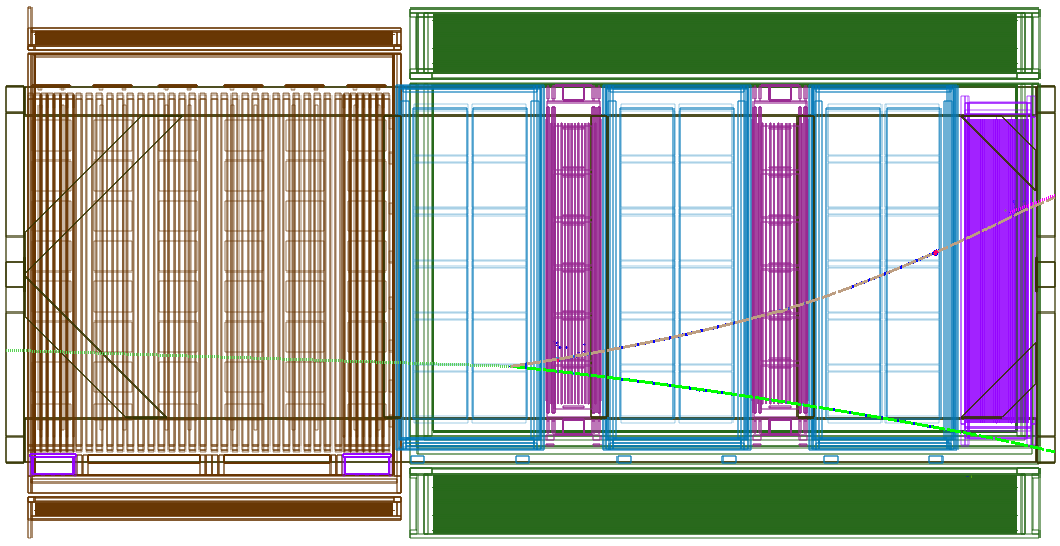
\includegraphics[width=0.8\linewidth]{goodeventMC}}
    \caption{Example of simulated event from HNL decay in the first TPC. Dashed green line corresponds to HNL track, green line to the muon track, brown line to the pion track.}
    \label{fig:HNL:event}
\end{figure}

\chapter{HNL analysis}
\label{ch:HNL:ana}

The search for heavy neutrinos consists of several steps. After the generation on the signal sample described in the previous chapter, the event selection can be developed. I don't expect too much background from the active neutrino interactions as we are using the fiducial volume of the atmospheric pressure TPC as the main detector. But because of the intense T2K neutrino beam some neutrinos will still interact there. The cut sequence to pick up the signal events and reject the background was developed to gain the sensitivity of the analysis.

An accurate systematic uncertainty evaluation is required to put robust upper limits on the HNL mixing elements. In our study, we use only HNL flux prediction simulation and detector efficiency to obtain the final results. Thus these two estimations are the only sources for the possible uncertainties. The systematics of kaon production have been studied in the other T2K analysis and can be applied in a straightforward way for the HNL analysis. The detector systematic needs to be studied more carefully. All the differences between the expected and observed detector behavior should be considered as an uncertainty. More details are provided in \autoref{sec:HNL:sys}.

\section{Event selection}
\label{sec:HNL:sel}
According to my analysis strategy, the background is severely suppressed by the fiducial detector choice. Very few active neutrino interactions are expected in the atmospheric pressure TPCs. But still, some of them are possible. The most dangerous are pion production as they are very similar to the expected signal. The vertex migration from the other detector is another possible reason for false HNL detection. The cut sequence is divided into two main parts: basic and advanced.

In the basic part, I select a pattern that is expected to be observed from the signal of interest. For example, for the $N\to\mu\pi$ decay, a vertex with two tracks should be reconstructed in the TPC fiducial volume. The particles should be oppositely charged and properly identified with the dE/dx in the gas. This part of the selection is referred to as ``basic '' as all the criteria came directly from the expected signal pattern. No cut changes are expected in this part.

The ``advanced'' part of the selection is dedicated to the separation between the signal and the background. First of all the veto cuts should be defined. As we are looking for the neutral particle decay the upstream activity may serve as good veto criteria. Then I am going to study the kinematics spectra for both signal and background samples and find the most optimum cut values to gain the analysis sensitivity. We expect the most powerful background reduction from the cut on the reconstructed heavy neutrino direction. The decay of neutral particles is expected to be extremely collinear with the beam axis while the active neutrino interactions will produce particles in the wide angular range.

\subsection{Cuts description}
The ``basic'' selection searches for the signal-like pattern in the TPC fiducial volume. The following cut sequence is defined:

\begin{enumerate}
  \item Vertex in the TPC fiducial volume.
  \item Two oppositely charged tracks associated with this vertex;
  \item Proper particle identification (PID) as $e\pi$ or $\mu \pi$ using $dE/dx$ in the TPC;
\end{enumerate}

With such a simple selection I would like to keep as many signal events as possible. Any signal event is expected to match the criteria above. The efficiency loss can be caused only by the wrong reconstruction.

The vertex requirement is a key point of the selection. The tracks matching into the vertex is performed with Kalman filter. It appeared that this requirement causes a dramatic efficiency reduction. Only 40\% of signal events pass the first cut. It happens because T2K TPCs are not optimized for the reconstruction of close tracks. The HNL decay is usually very relativistic and the daughter particles have a very small opening angle (\autoref{fig:HNL:secondary}). The length of the TPC is about 70 cm. Sometimes it is not enough for the robust track spiting despite the good spatial resolution of the detector. The HNL decay points are distributed uniformly over the TPC volume that makes the situation even worse. Quite often it is placed close to the downstream scintillator detector. The resolution of the latter is limited by the scintillator bar size. Quite often the outgoing pion can interact inside the scintillator detector that makes the vertex reconstruction completely impossible unless lepton and pion tracks were separated enough in the TPC volume.
%As a result, the event looks like a scattering with secondary particle production. While in fact, it is a decay, but the decay products are separated by the detector far away from the vertex.

\begin{bclogo}[couleur=blue!2, arrondi=0.1, logo=\bcinfo, nobreak=true]{Vertexing with Kalman filter}
    The Kalman filter is a recursive filter that estimates the internal state of a dynamic system from number of noisy measurements. Originally it was developed for the rocket science and is still actively used in this field. The flow of the method is shown in \autoref{fig:HNL:kalman}. As one can see we start with the prior measurements, make a prediction about the next step based on the model, then correct the prediction with the actual measurement.

    In the case of the vertex finding in the detector the model is the track propagation through the detector in magnetic field. For the prior we extrapolate the reconstructed tracks to the closest intersection point. Then we go through several iterations using the observed detector hits as a data. At the end we arrive to the precise reconstruction of the vertex position with the know uncertainty and the quality of the fit.
\end{bclogo}

\begin{figure}[!ht]
  \center{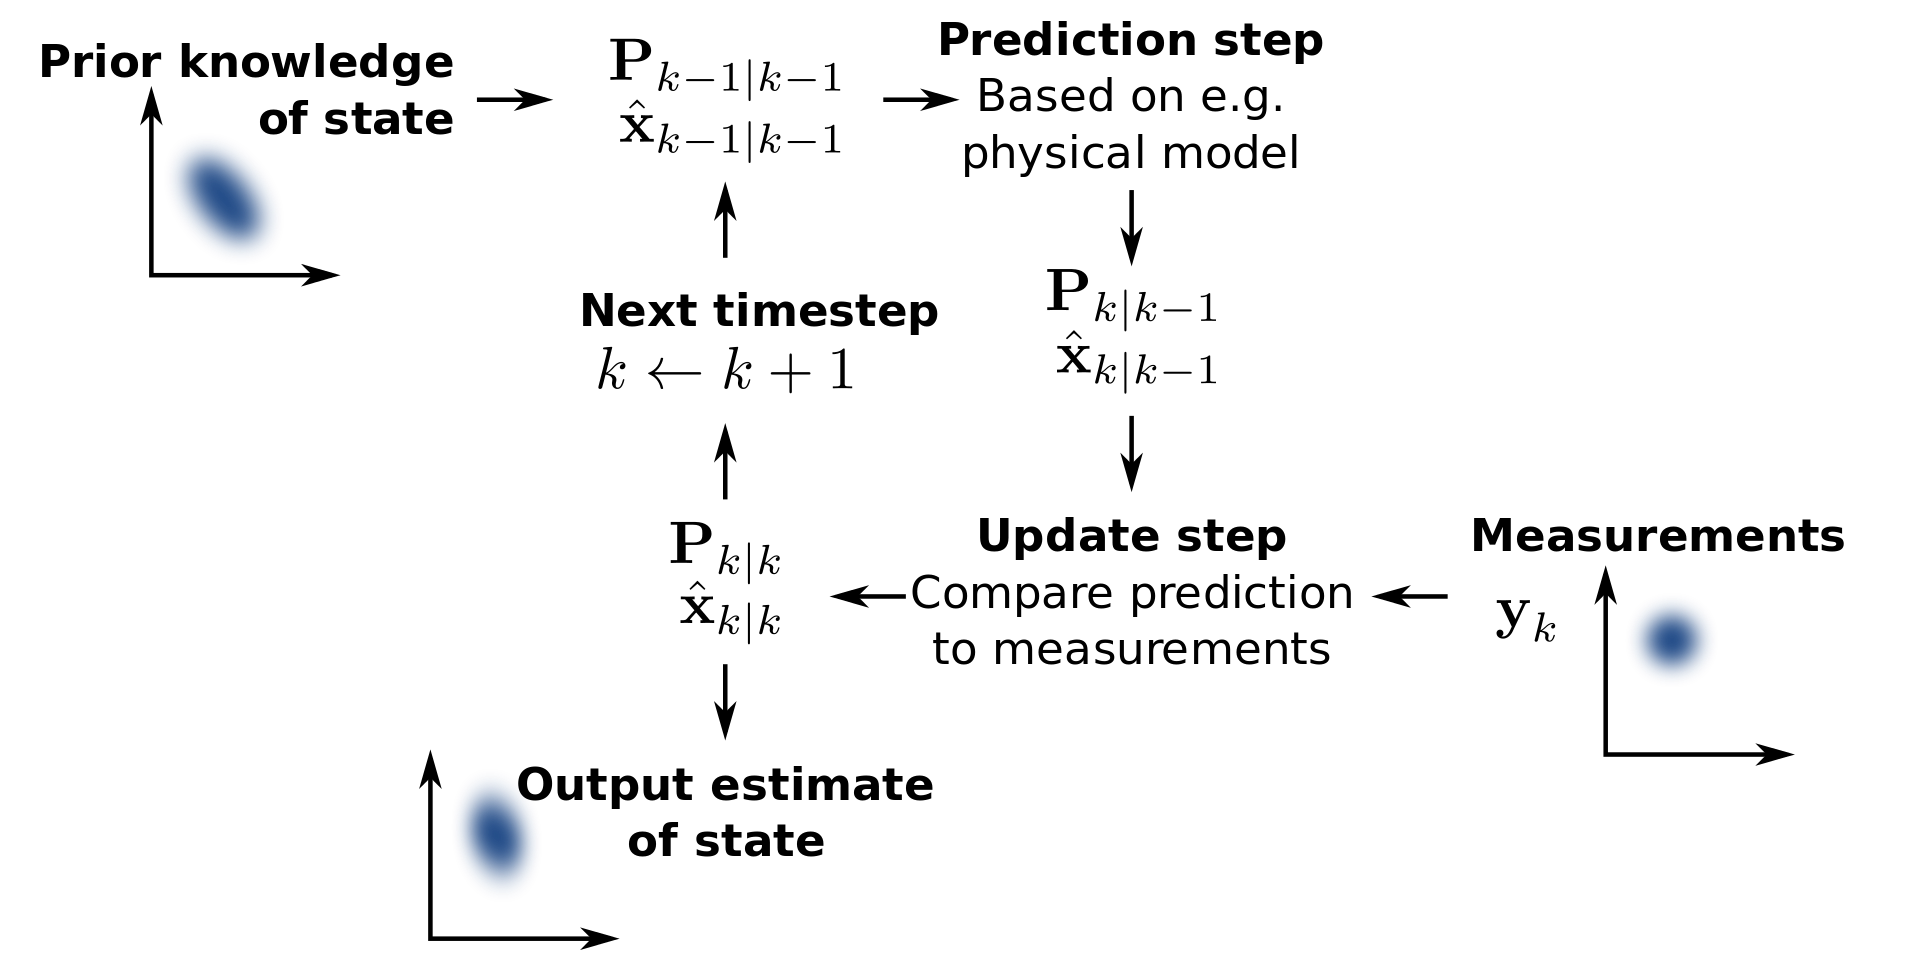
\includegraphics[width=0.6\linewidth]{kalman.png}}
  \caption{The flow of the Kalman filter usage.}
  \label{fig:HNL:kalman}
\end{figure}

The second cut that rejects many signal events is particle identification. I use the energy loss in the TPC (dE/dx) to determine the particle type. In ND280 detector the particle identification is done with the likelihood function comparison. Four hypotheses are built with the comparison of the expected and observed energy loss for electron, muon, pion, and proton. The problem occurs in certain kinematics regions where the energy loss is similar for the different particles. E.g. proton and muon/pion can be confused at the momentum around 1.5 GeV/c. Also, positron and proton have very similar dE/dx at a momentum around 1 GeV/c. Though the particle identification works quite well it is the second cut that most reduces the HNL selection efficiency.

The ``advance'' part of the selection is aimed at the background reduction. The following cuts are applied:

\begin{itemize}
  \item No activity in the upstream detector;
  \item No other tracks start in the same TPC;
  \item Invariant mass cut: e.g. $140MeV<M_{HNL}<850MeV$ for the $e\pi$ mode
  \item Polar angle for HNL candidate: e.g. $\theta < 8.0^\circ$ for the $e\pi$ mode
  \item Opening angle between daughter particles $cos\theta >0.00$;
\end{itemize}

These requirements affect very little the signal selection efficiency but are essential for the background reduction. The neutrino interaction can take place in the upstream detector but due to the reconstruction failure, the vertex can be placed in the TPC fiducial volume. To reject such an event any upstream activity is used as a veto and event is not considered as a signal. The other source of the backgrounds is the inefficient track matching into the vertex. For example, an active neutrino interacts in the TPC volume but more than two tracks are produced. Sometimes vertex matching algorithm can associate only two tracks with the vertex and leave the others unassigned. To reject this process I require no other activity in the TPC besides two tracks that are matched with the HNL candidate decay vertex.

The most powerful cuts for background rejection are the kinematic cuts. The reconstructed invariant mass should be in the kinematically allowed region. Since we are looking for the HNL from kaon decay it can not exceed 493 MeV/$\text{c}^2$. But ND280 can not measure the invariant mass of the HNL in a precise way. Some tolerance is needed to keep efficiency high enough. Nevertheless, this cut is powerful for neutrino interaction rejection since this process can cause the ``invariant mass'' to be in a very wide range.

The reconstructed direction of the HNL candidate is expected to be parallel to the neutrino beam. The products of the neutrino interaction can be distributed in a wide angle. Neutrino interactions are affected by the nuclear effect thus the invariant direction is biased w.r.t. neutrino beam direction. I studied the distribution of the polar angle of the HNL candidate for events that passed all previous cuts, as it is the most strict kinematic cut. Then we looked at the opening angle of the HNL candidate daughters. The results are presented in \autoref{fig:HNL:kin1} and \autoref{fig:HNL:kin2}.

\begin{figure}[!ht]
  \begin{minipage}[h]{0.49\linewidth}
    \center{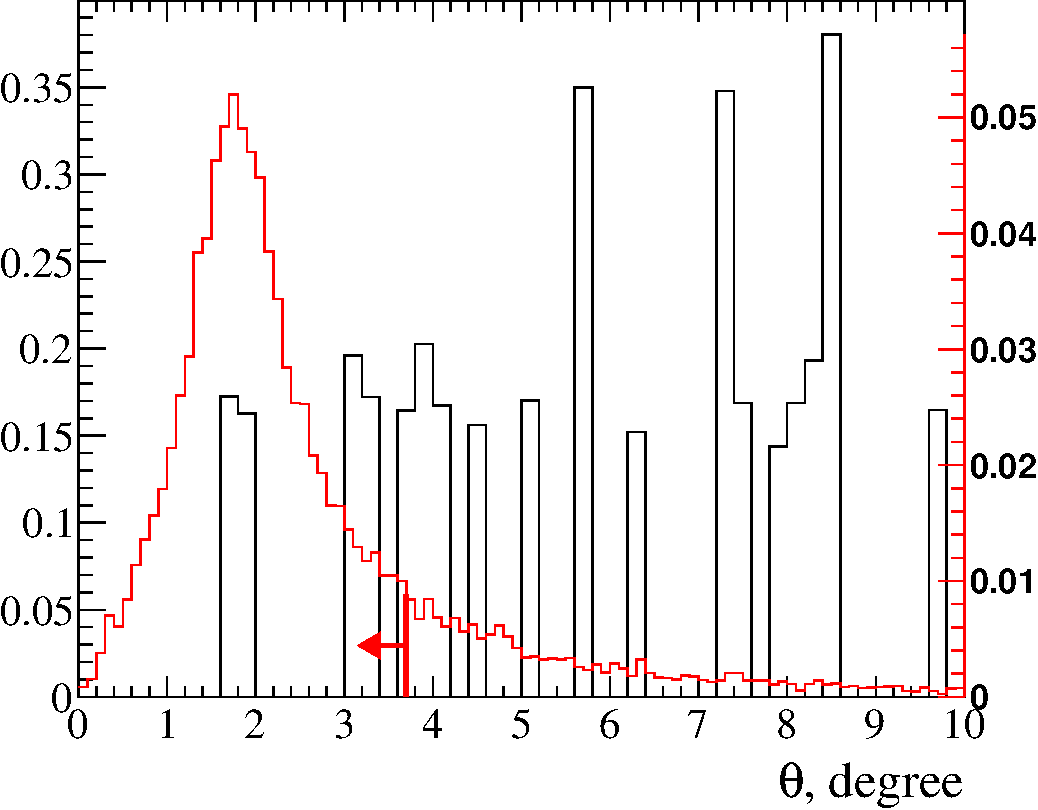
\includegraphics[width=\linewidth]{HNLpolarMu}  \\ a)}
  \end{minipage}
  \hfill
  \begin{minipage}[h]{0.49\linewidth}
    \center{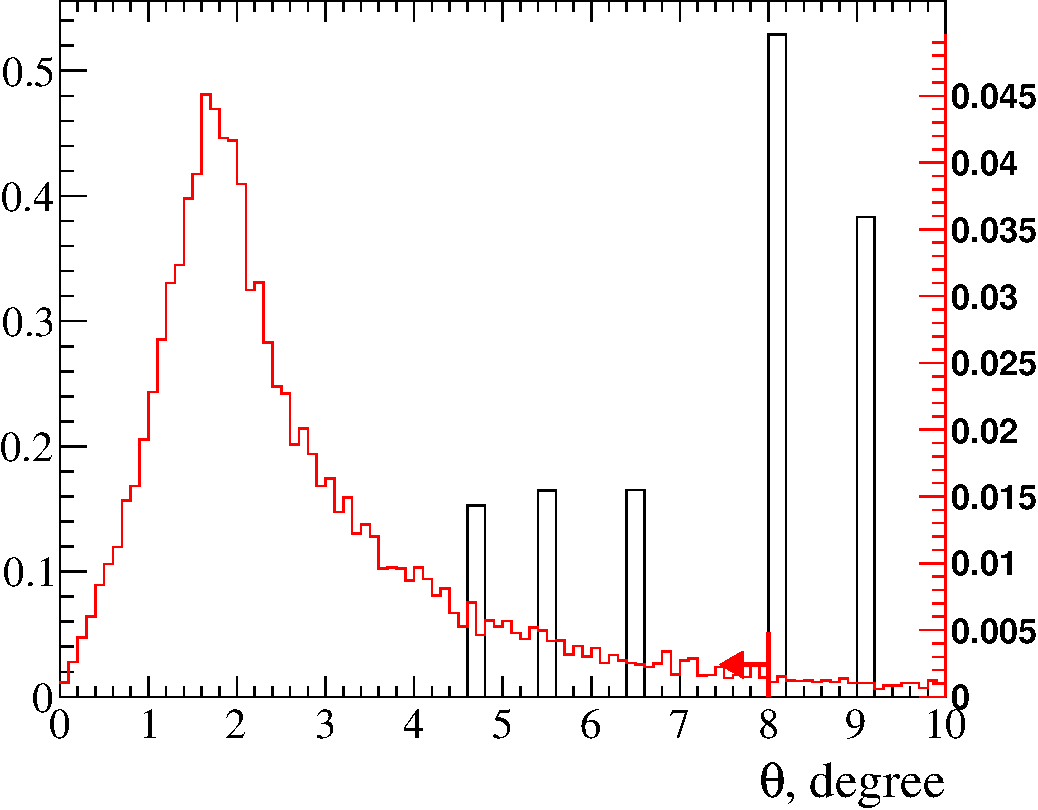
\includegraphics[width=\linewidth]{HNLpolarEle}  \\ b)}
  \end{minipage}
  \caption{Angular distribution of the HNL candidate events (a) for $\mu\pi$ mode and (b) for $e\pi$. Red is the signal samples, black is the background from the neutrino interactions and vertical line is a cut value. Background spectrum is normalized to $10^{21}POT$, signal is normalized to 1.}
  \label{fig:HNL:kin1}
\end{figure}

\begin{figure}[!ht]
  \begin{minipage}[h]{0.49\linewidth}
    \center{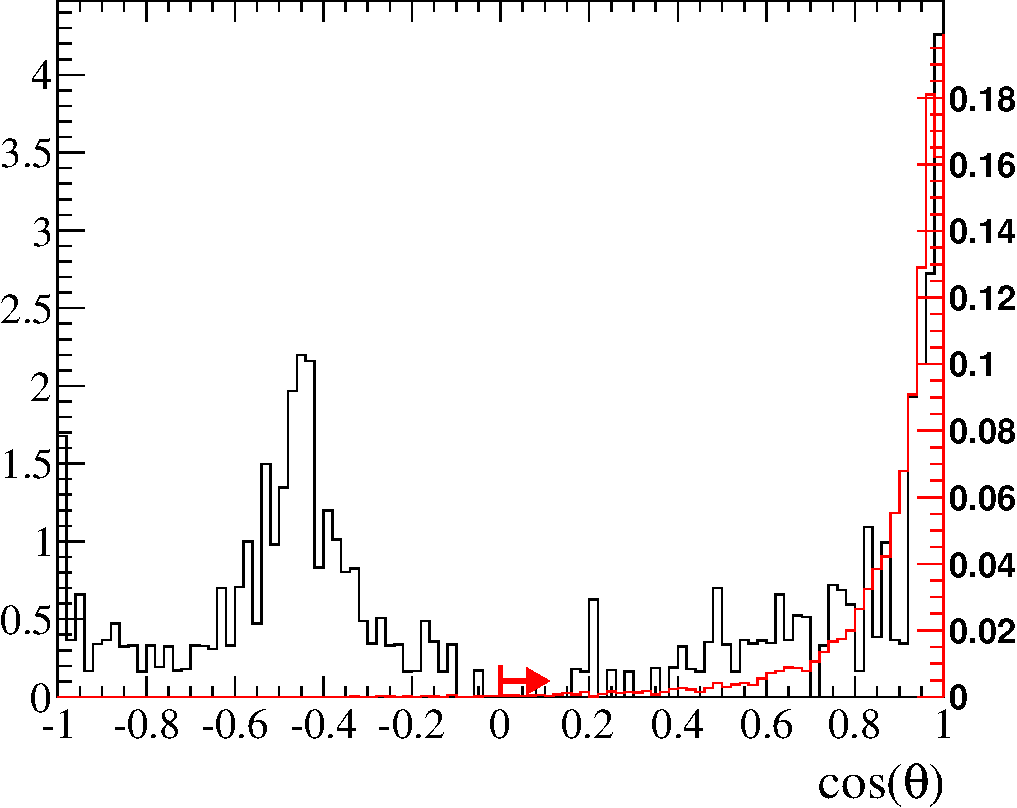
\includegraphics[width=\linewidth]{HNLrelative1} \\ a)}
  \end{minipage}
  \hfill
  \begin{minipage}[h]{0.49\linewidth}
    \center{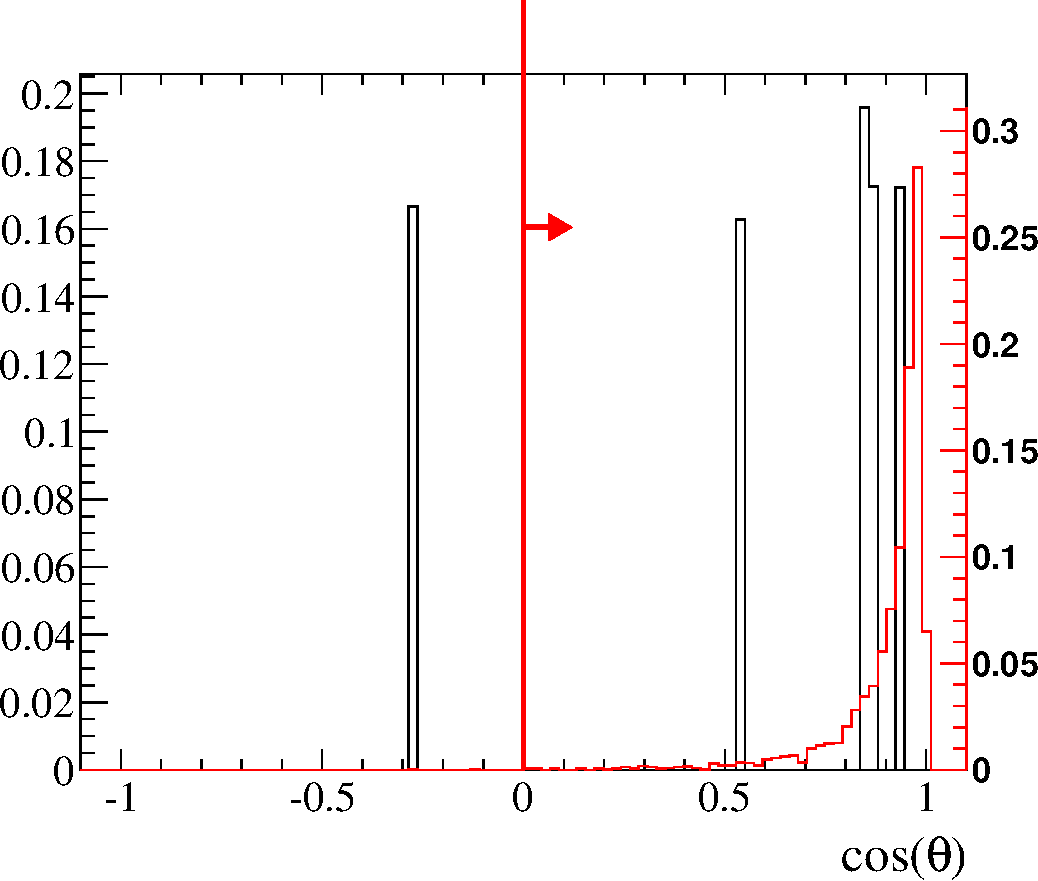
\includegraphics[width=\linewidth]{HNLrelative2} \\ b)}
  \end{minipage}
  \caption{Opening angle for the HNL daughter particles for the $\mu\pi$ mode (a) before the polar angle cut was applied and (b) after. Red is the signal samples, black is the background from the neutrino interactions and vertical line is a cut value. The background is normalized to $10^{21}POT$, the signal is normalized to 1.}
  \label{fig:HNL:kin2}
\end{figure}

\subsubsection{\texorpdfstring{$N\to\mu\mu\nu$}{Lg}  mode cuts}
The dimuon mode requires a special selection. Two muons can not be produced in the neutrino interactions and I want to use the benefits of that fact. But it is not possible to distinguish a muon from a pion using the energy loss in the TPC. So I decided to use the ECal. Pions are expected to cause a shower in the calorimeter while a muon will leave a clean track. So an additional cut was applied. Each muon candidate should reach ECal and behave as a track there. The kinematics cuts were also reviewed. The three-body decay with a neutrino will not allow reconstructing the HNL direction as precisely as a two-body decay. So less strict cut on the polar angle was set.

\subsection{Signal selection efficiency}
\label{sec:HNL:eff}

Applying all these cuts to the signal samples give us the total selection efficiency (\autoref{fig:HNL:Eff1}, \autoref{fig:HNL:Eff2}). The efficiency of the HNL selection in my analysis is defined as a ratio of the number of the selected events to the number of the generated HNL events inside the TPCs fiducial volume. The main reason for the dependence of the efficiency on the HNL mass is track reconstruction. For the large HNL mass, we have more events with successfully reconstructed tracks associated with the decay vertex.

\begin{figure}[!ht]
  \begin{minipage}{0.49\linewidth}
    \centering{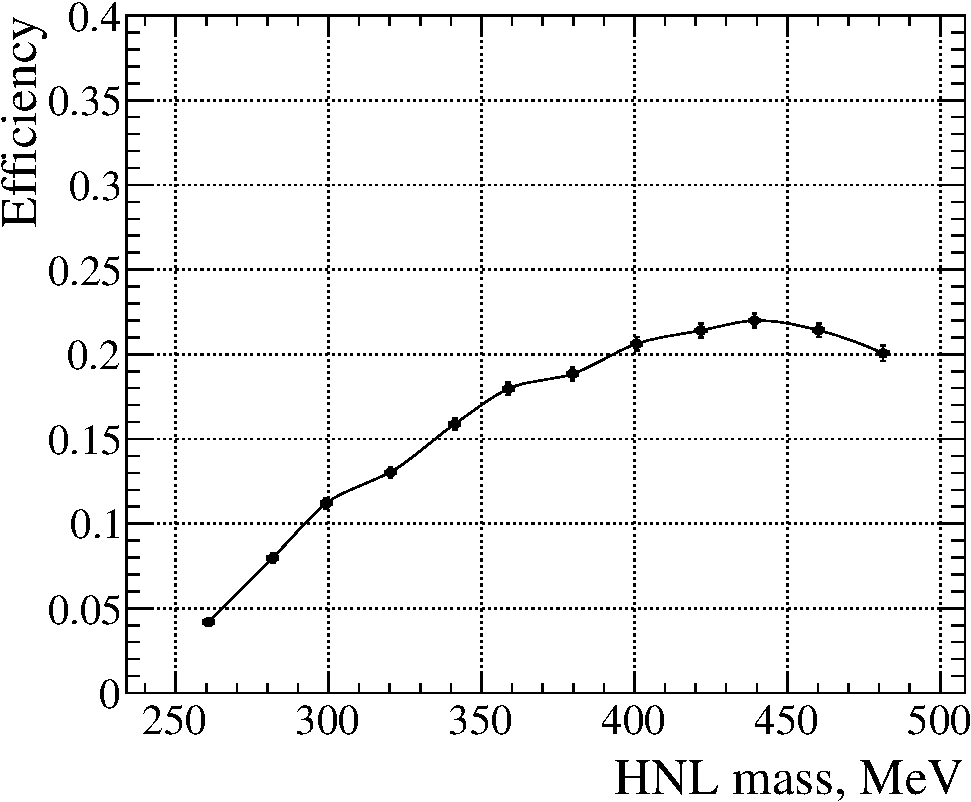
\includegraphics[width =\linewidth]{EffMu} \\ $K^+\to e^+N\to e^+\left(\mu^\mp\pi^\pm\right)$}
  \end{minipage}
  \hfill
  \begin{minipage}{0.49\linewidth}
    \centering{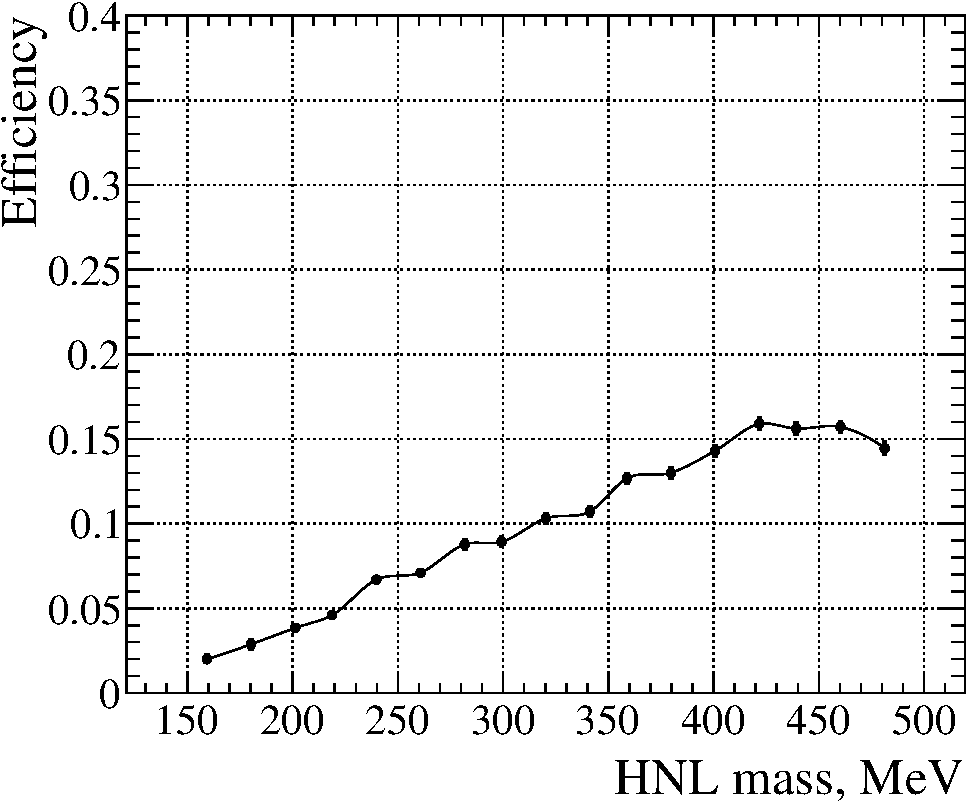
\includegraphics[width =\linewidth]{EffEle} \\ $K^+\to e^+N\to e^+\left(e^\mp\pi^\pm\right)$}
  \end{minipage}
  \caption{Selection efficiency for two body decays of HNL.}
  \label{fig:HNL:Eff1}
\end{figure}

\begin{figure}[!ht]
   \centering{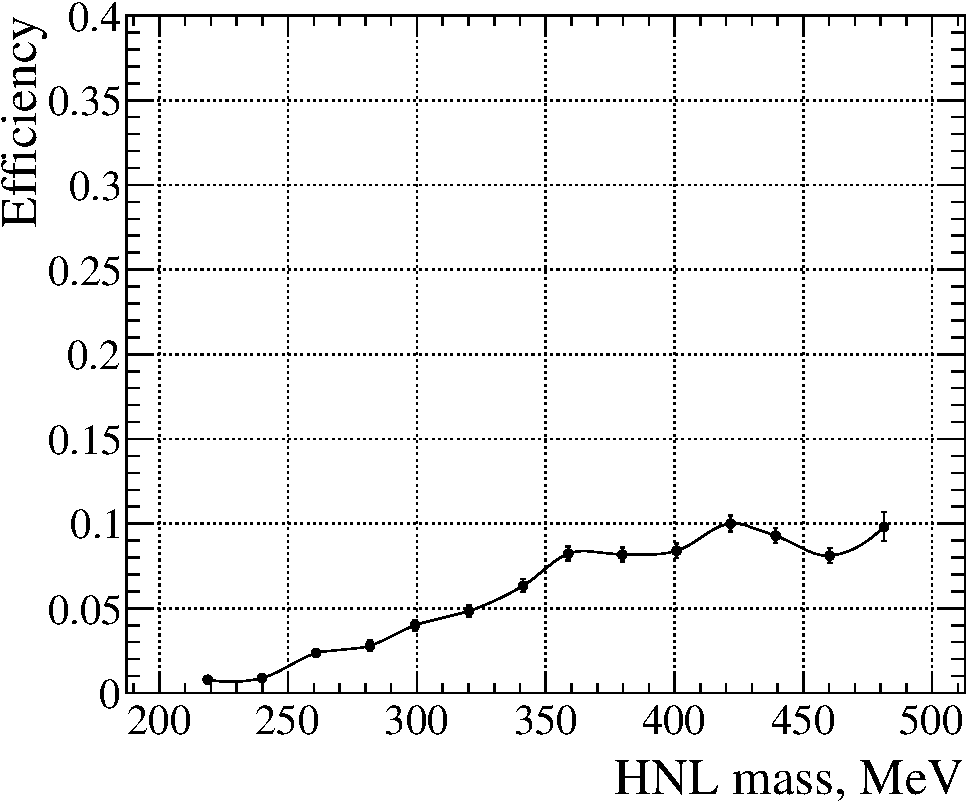
\includegraphics[width =0.4\linewidth]{EffDimuon}}
  \caption{Selection efficiency for HNL decay mode $N\to\mu\mu\nu$.}
  \label{fig:HNL:Eff2}
\end{figure}

The efficiency dependence on different cuts is shown in \autoref{fig:HNL:EffDrop}. The main drop is caused by the inefficient track matching algorithm. As was mentioned above HNL decay cause two close tracks that are difficult to separate with ND280.

\begin{figure}[!ht]
  \centering{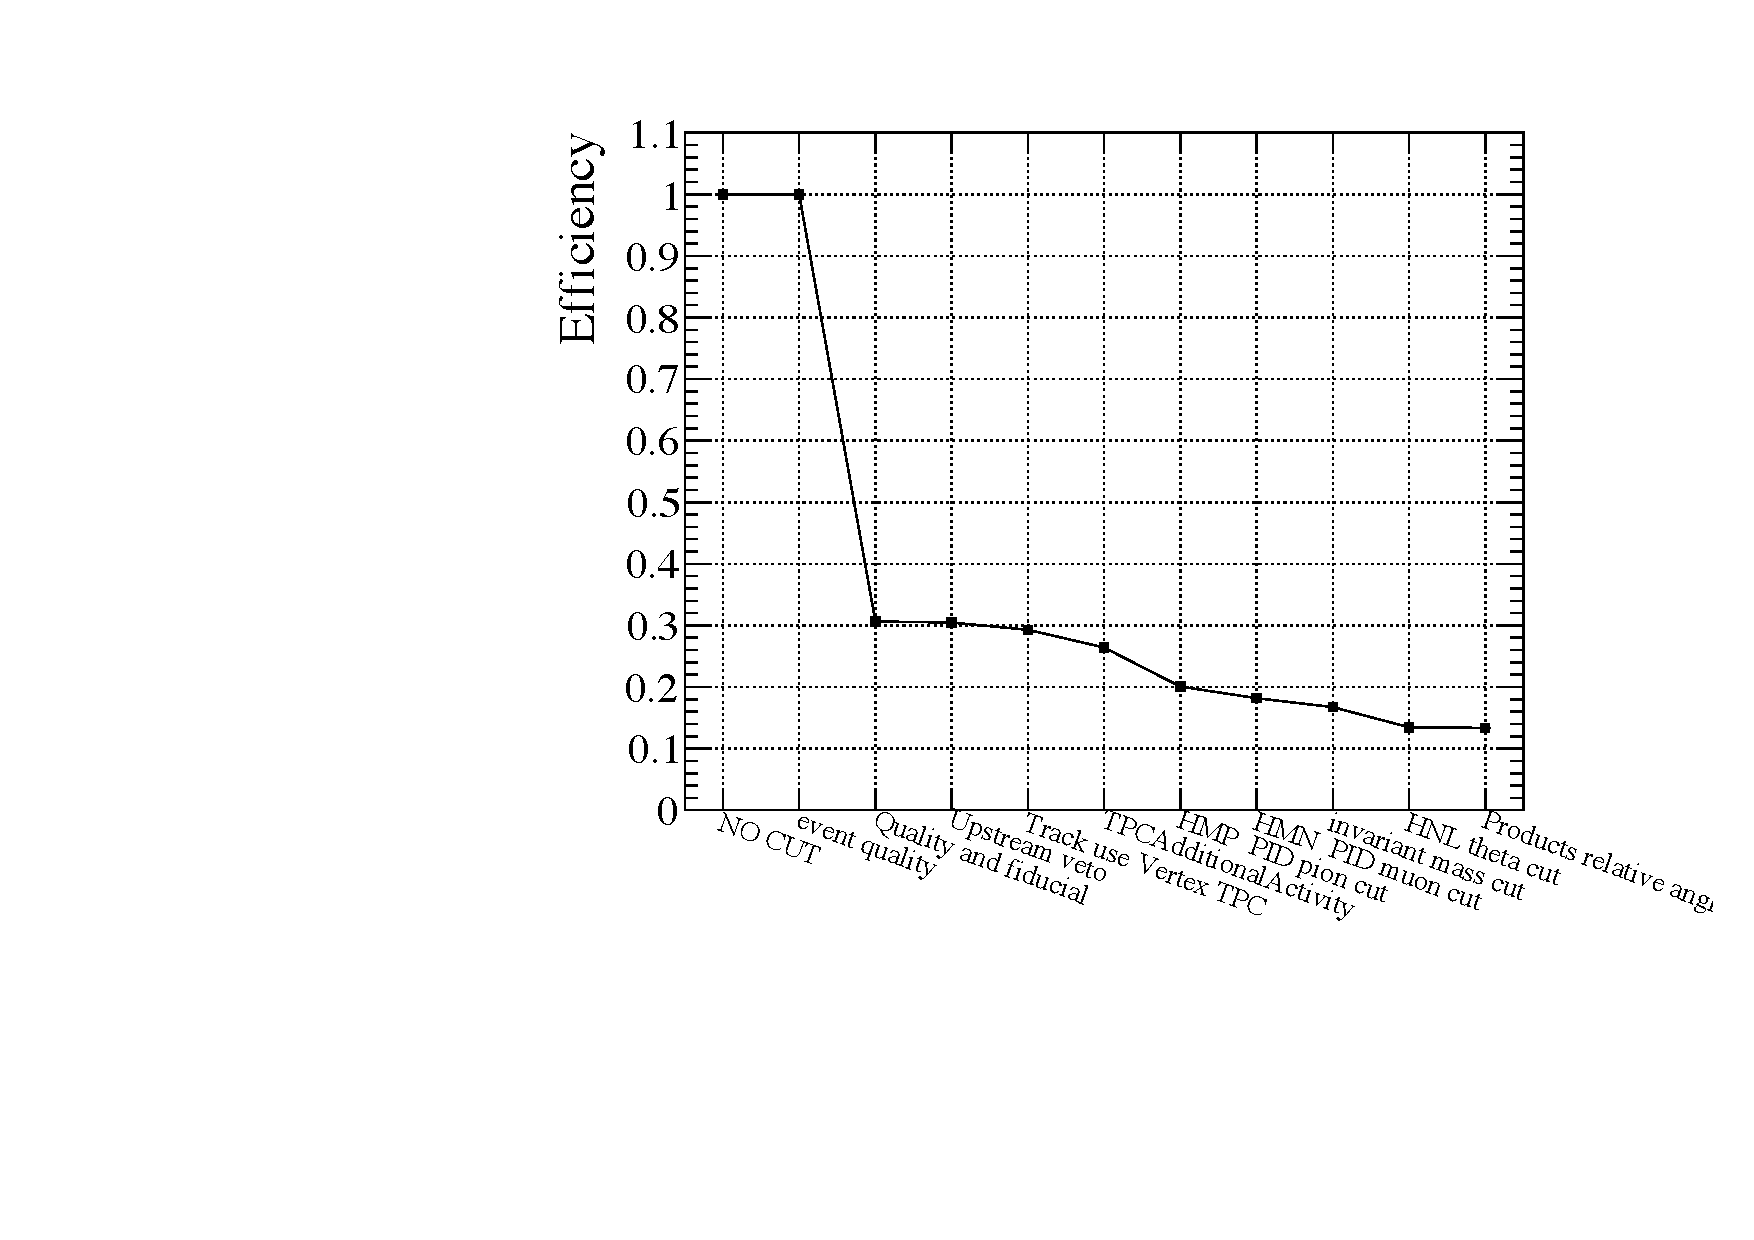
\includegraphics[width = 0.6\linewidth]{EffDrop}}
  \caption{Efficiency dependence on the applied cuts for mode $N\to\mu^\mp+\pi^\pm$ for all HNL masses.}
  \label{fig:HNL:EffDrop}
\end{figure}

The dependence of the efficiency on the HNL momentum and opening angle of the daughter particles is shown in \autoref{fig:HNL:EffDep}. As expected the maximum efficiency is for HNL with momentum below 2 GeV/c. The TPCs were designed for the event reconstruction in this momentum region.
\begin{figure}[!ht]
  \begin{minipage}{0.49\linewidth}
    \centering{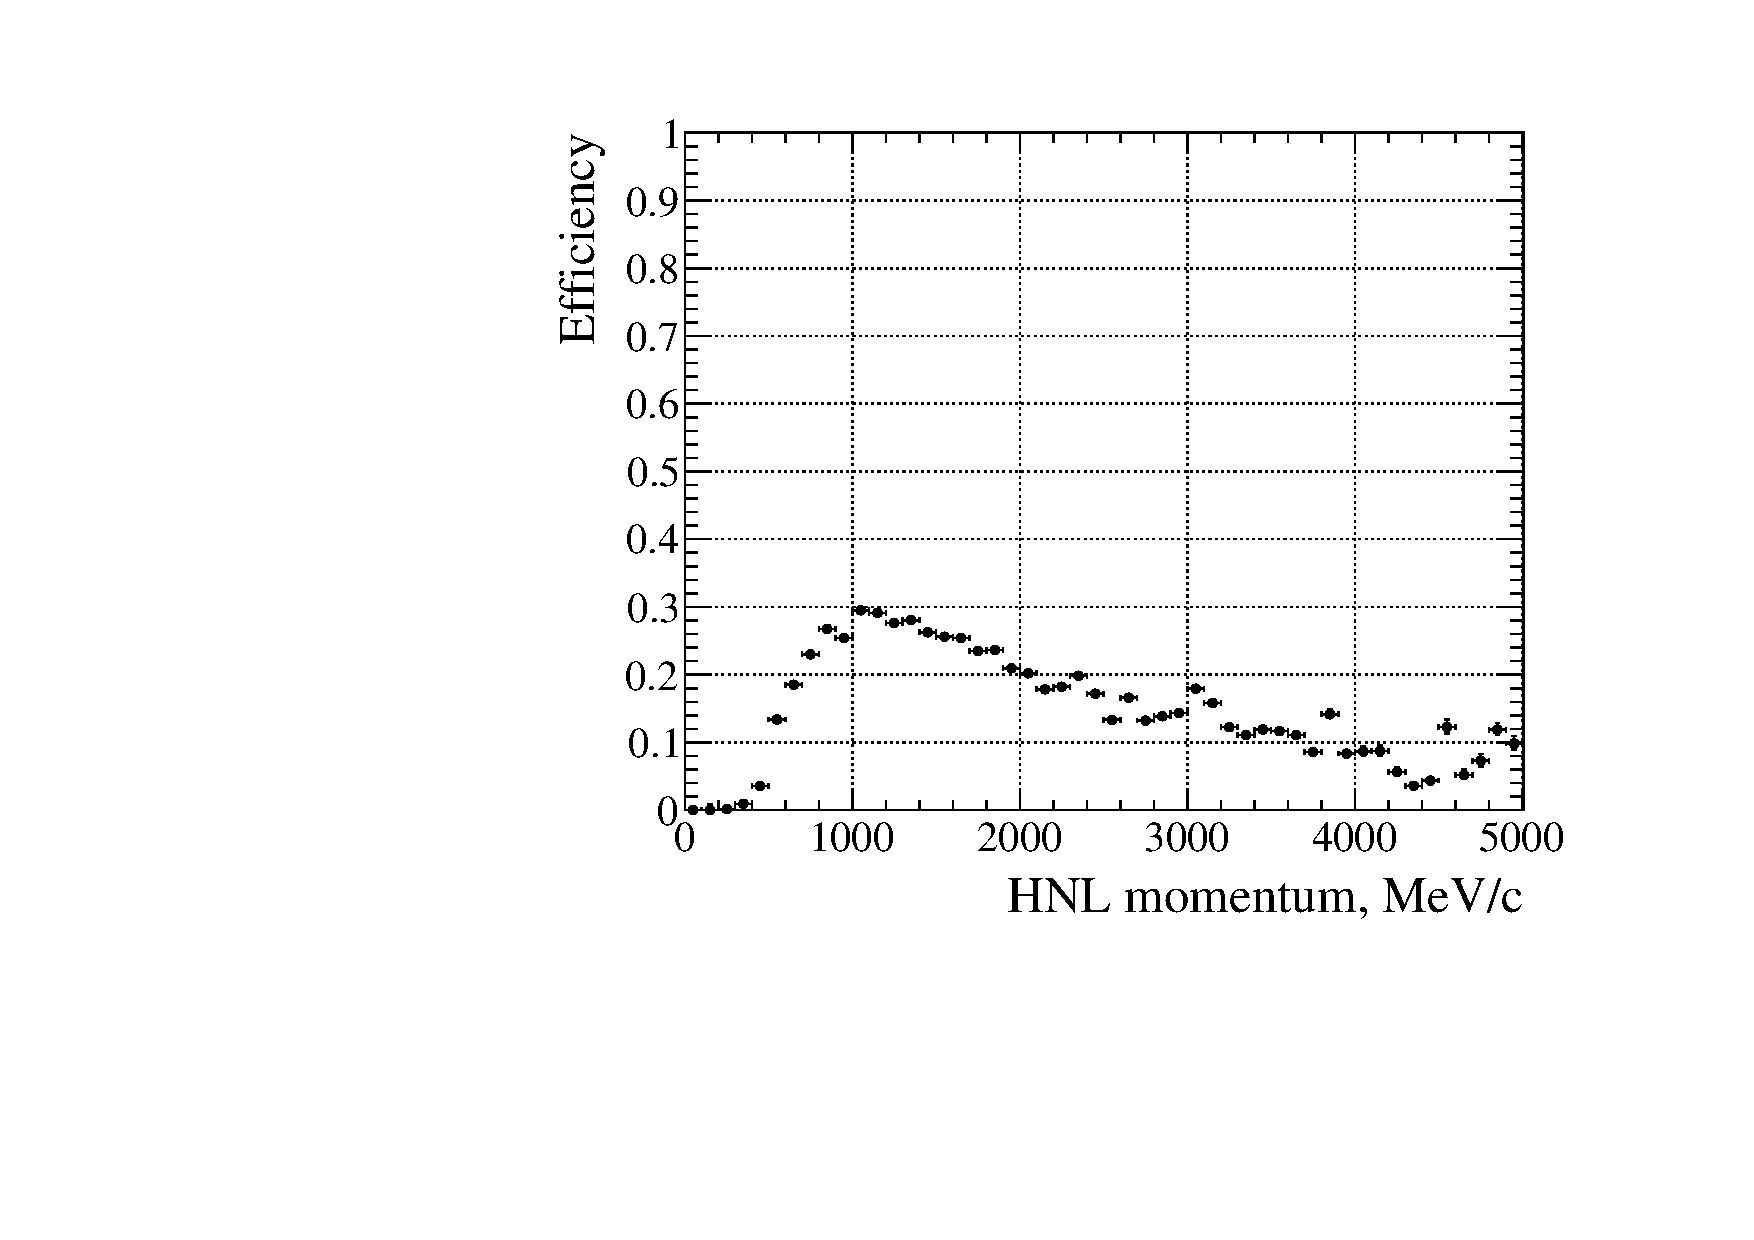
\includegraphics[width =\linewidth]{EffMom} \\ a)}
  \end{minipage}
  \hfill
  \begin{minipage}{0.49\linewidth}
    \centering{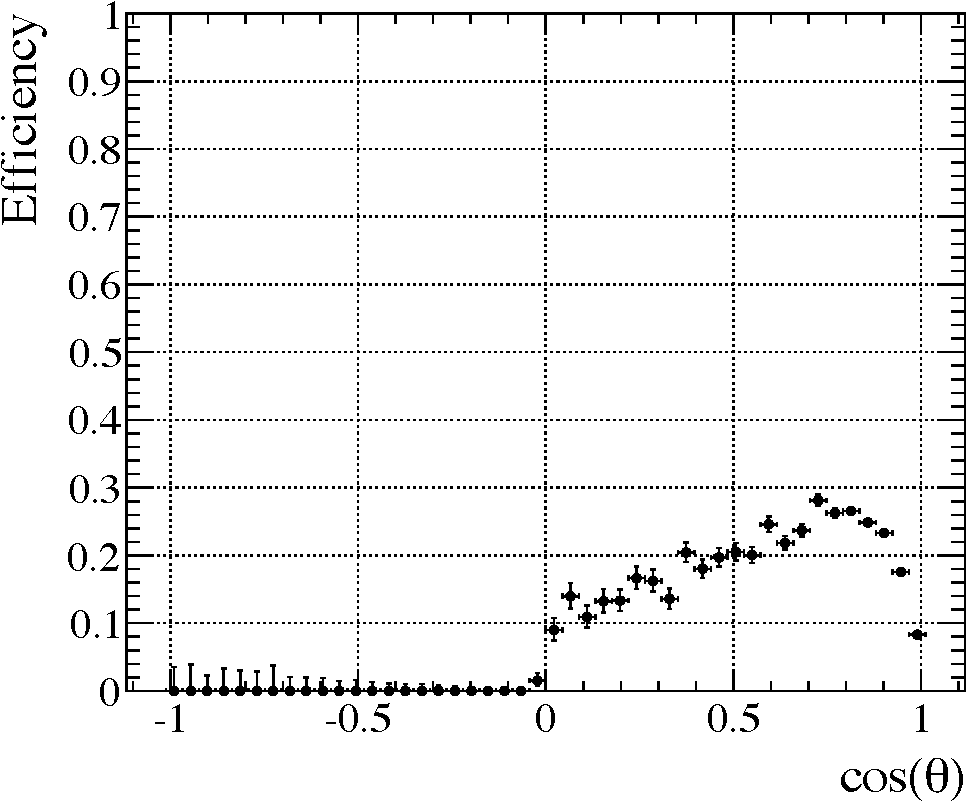
\includegraphics[width =\linewidth]{EffCos} \\ b)}
  \end{minipage}
  \caption{The dependence of efficiency for mode $N\to\mu\pi$: (a) on the HNL momentum and (b) opening angle of daughter particles.}
  \label{fig:HNL:EffDep}
\end{figure}

Since we study the HNL production from $K^+$,  $K^-$ and their decays into $\ell^{\pm}h^{\mp}$, the efficiency should be evaluated for every mode. Such a result is presented in \autoref{fig:HNL:C_check}. We can see the agreement of the efficiency study for the different channels.

\begin{figure}[!ht]
  \begin{minipage}{0.49\linewidth}
    \centering{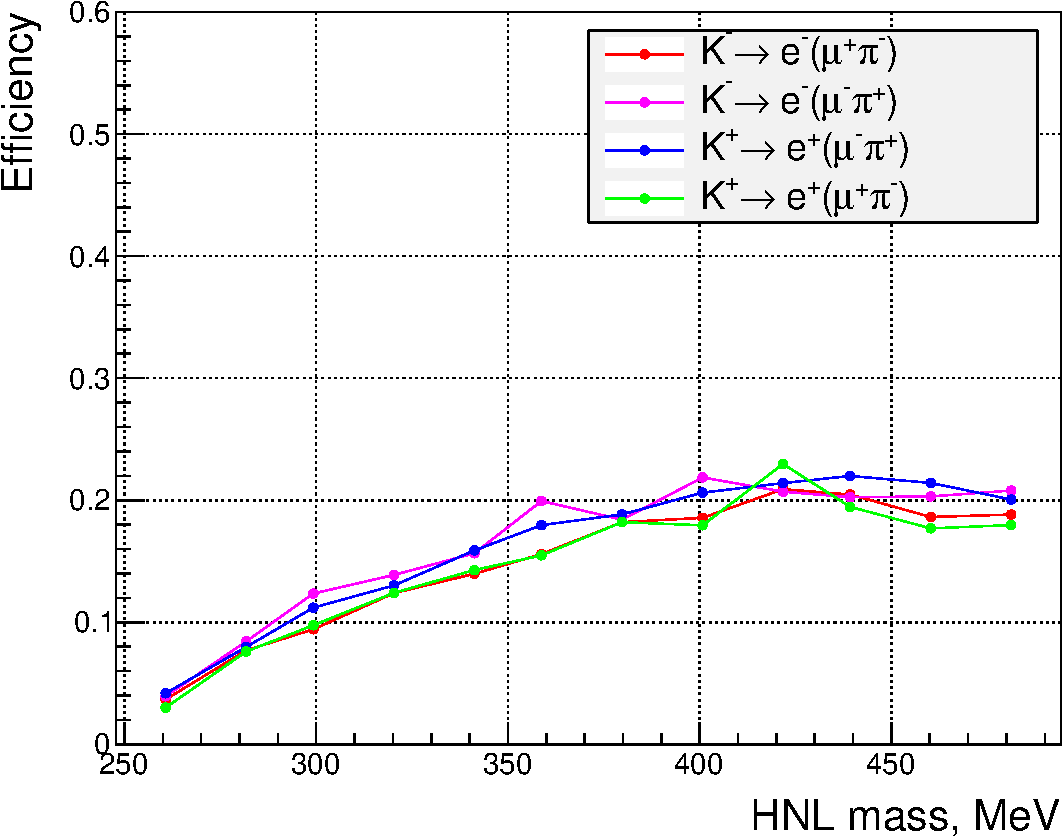
\includegraphics[width =\linewidth]{C_checkMu} \\ $N\to \mu\pi$}
  \end{minipage}
  \hfill
  \begin{minipage}{0.49\linewidth}
    \centering{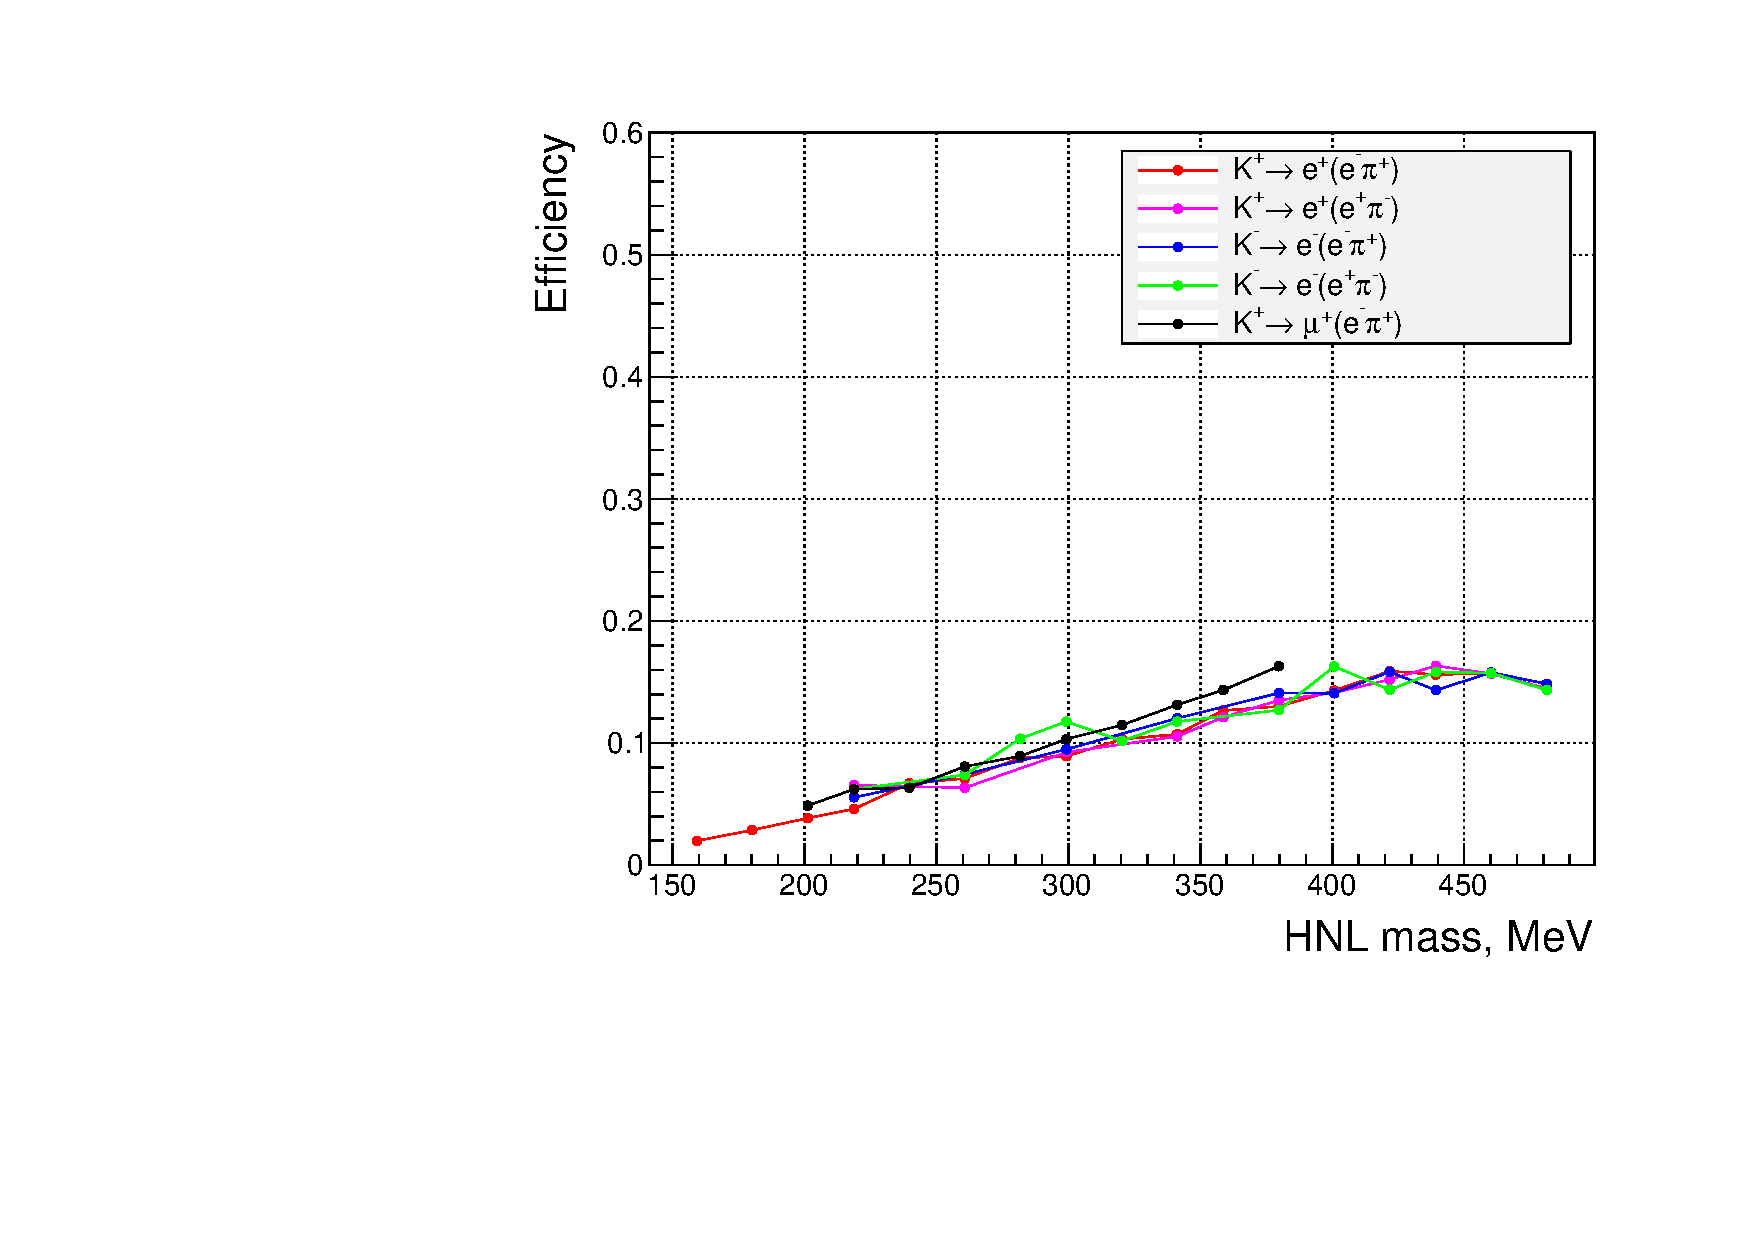
\includegraphics[width =\linewidth]{C_checkEle} \\ $N\to e\pi$}
  \end{minipage}
  \caption{HNL selection efficiencies for several production and decay modes.}
  \label{fig:HNL:C_check}
\end{figure}

\subsection{Background suppression}
\label{sec:HNL:bg}
In the T2K experiment neutrino interactions in the ND280 had been already simulated. Different neutrino generators had been used to consider several different models. In our study we are affected by the poorly studied processes of pion production in the gaseous Argon. Thus I used all the available generators and compared the results to minimize the model dependence. NEUT~\cite{Hayato2002}, GENIE~\cite{Andreopoulos2010}, and NuWro~\cite{Zmuda2015} toolkits were used for background estimation. For example, GENIE is believed to be more accurate in kaon production prediction, while I expected the neutral kaon decay $K^0_L\to\ell\pi\nu_\ell$ to mimic the signal process. The statistics used for the Monte--Carlo simulation is nearly ten times bigger than the data collected in the experiment. Thus I am going to study the background with small statistical uncertainties. The background is divided into neutrino interaction types. Remaining backgrounds after each cut as well as a signal efficiency are summarized in \autoref{tbl:HNL:bgOrigMu} and \autoref{tbl:HNL:bgOrigEle}.

\begin{table}[!ht]
%\begin{adjustbox}{width=1.1\linewidth,center}
\begin{tabular}{|c|l|r|r|r|r|r|r|r|r|r|r|r|}
  \hline
  N & Cut           &  CCQE   &  RES  &  DIS  &  COH  &  NC  &  2P2H  &  OOFV  &$\bar{\nu_{\mu}}$& $\nu_{e}$ & Total  & Eff\\
  \hline
  1 & Vertex        & 140.11  & 30.88 & 20.34 & 4.57  & 8.48 & 1.65   & 647.31 & 2.39            &  3.63     & 859.34 & 44.0 \\
  \hline
  2 & Veto          &  122.44  & 21.24 & 10.75 & 3.89  & 6.55 & 0.82   & 281.47 & 1.80            &  2.43     & 451.39 & 39.1 \\
  \hline
  3 & PID           & 5.08    & 5.51  & 5.60  & 2.03  & 1.25 & 0.00   & 48.64  & 1.37            &  0.19     &  69.66 & 31.3 \\
  \hline
  4 & Inv mass      & 0.83    & 3.52  & 2.17  & 1.67  & 0.90 & 0.00   & 43.17  & 0.92            &  0.00     &  53.18 & 29.2  \\
  \hline
  5 & Kinematic     & 0.00    & 0.17  & 0.20  & 0.34  & 0.00 & 0.00   & 0.00   & 0.00            &  0.00     &  0.70  & 21.1 \\
    \hline

\end{tabular}
\caption{The number of MC background events after every cut for $10^{21} POT$ from NEUT generator for $\mu\pi$ mode. The budget is split into quasi--elastic processes (CCQE), resonance $\pi$ production (RES), coherent $\pi$ production (COH), deep inelastic interaction (DIS), neutral current interactions (NC), out of fiducial volume interactions (OOFV), $\overline{\nu}_\mu$ and $\nu_e$ interactions.}
\label{tbl:HNL:bgOrigMu}
%\end{adjustbox}
\end{table}

The main background for the $N\to\mu\pi$ decay channel is pion production as was expected. Some contribution from deep inelastic processes was also observed. The veto cuts demonstrate it's high efficiency rejecting lots of active neutrinos but keeping the signal efficiency nearly the same.


\begin{table}[!ht]
%\begin{adjustbox}{width=1.1\linewidth,center}
\begin{tabular}{|c|l|r|r|r|r|r|r|r|r|r|r|r|}
  \hline
  N & Cut           &  CCQE   &  RES  &  DIS  &  COH  &  NC  &  2P2H  &  OOFV  &$\bar{\nu_{\mu}}$& $\nu_{e}$ & Total  & Eff\\
  \hline
  1 & Vertex        & 140.11  & 30.88 & 20.34 & 4.57  & 8.48 & 1.65   & 647.31 & 2.39            &  3.63     & 859.34 & 34.5 \\
  \hline
  2 & Veto          & 122.44  & 21.24 & 10.75 & 3.89  & 6.55 & 0.82   & 281.47 & 1.80            &  2.43     & 451.39 & 31.1 \\
  \hline
  3 & PID          & 5.74    & 0.17  & 0.92  & 0.17  & 0.20 & 0.00   & 13.91  & 0.00            &  0.00     &  21.11 & 17.8 \\
  \hline
  4 & Inv mass      & 0.66    & 0.17  & 0.37  & 0.17  & 0.20 & 0.00   & 13.32  & 0.00            &  0.00     &  14.87 & 17.1  \\
  \hline
  5 & Kinematic     & 0.00    & 0.00  & 0.00  & 0.17  & 0.00 & 0.00   & 0.32   & 0.00            &  0.00     &  0.48  & 14.8 \\
    \hline

\end{tabular}
\caption{The number of MC background events after every cut for $10^{21} POT$ from NEUT for $e\pi$ mode. The budget is split into quasi--elastic processes (CCQE), resonance $\pi$ production (RES), coherent $\pi$ production (COH), deep inelastic interaction (DIS), neutral current interactions (NC), out of fiducial volume interactions (OOFV), $\overline{\nu}_\mu$ and $\nu_e$ interactions.}
\label{tbl:HNL:bgOrigEle}
%\end{adjustbox}
\end{table}

For the $N\to e\pi$ mode, the main background process is expected to be different from the one for $N\to\mu\pi$ mode. Pion production is not so dangerous as in T2K the beam is almost pure. A pion production will always cause a muon production as well. Some contribution of the coherent pion production in the $N\to e\pi$ is caused by the wrong particle identification. But the main process is out of fiducial volume neutrino interactions. The neutral pion production is responsible for this contamination. $\pi^0$ decays almost immediately after the neutrino interaction and produce two gammas. One of the gammas can go downstream in the ND280 and convert in the next detectors. In case of the wrong particle identification of the $e^+e^-$ pair we can reconstruct the process as $e\pi$ production. Photons can travel through several subdetectors in ND280. Because of the high beam intensity I can not constrain all the activity in the ND280 as it will dramatically reduce the efficiency. Instead, I consider only the first upstream subdetector activity as a veto.

\begin{comment}
\begin{table}[!ht]
%\begin{adjustbox}{width=1.1\linewidth,center}
\begin{tabular}{|c|l|r|r|r|r|r|r|r|r|r|r|r|}
  \hline
  N & Cut           &  CCQE   &  RES  &  DIS  &  COH  &  NC  &  2P2H  &  OOFV  &$\bar{\nu_{\mu}}$& $\nu_{e}$ & Total  & Eff\\
  \hline
  1 & Vertex        & 140.11  & 30.88 & 20.34 & 4.57  & 8.48 & 1.65   & 647.31 & 2.39            &  3.63     & 859.34 & 42.1 \\
  \hline
  2 & Veto          & 136.47  & 27.86 & 17.58 & 4.25  & 8.15 & 1.65   & 514.72 & 2.10            &  3.45     & 716.23 & 42.0 \\
  \hline
  3 & Use TPC       & 135.77  & 27.31 & 17.19 & 4.25  & 8.15 & 1.48   & 505.18 & 2.10            &  3.45     & 704.88 & 40.5 \\
  \hline
  4 & TPC act.      & 122.44  & 21.24 & 10.75 & 3.89  & 6.55 & 0.82   & 281.47 & 1.80            &  2.43     & 451.39 & 38.2 \\
  \hline
  5 & PID 1         & 121.90  & 17.97 & 9.27  & 3.54  & 4.19 & 0.82   & 134.29 & 1.36            &  0.54     & 284.87 & 33.6 \\
  \hline
  6 & PID 2         & 4.38    & 5.01  & 5.22  & 1.70  & 0.91 & 0.00   & 27.59  & 1.08            &  0.91     &  46.09 & 22.5 \\
  \hline
  7 & Use ECal      & 2.12    & 1.79  & 1.89  & 0.68  & 0.34 & 0.00   & 2.56   & 0.33            &  0.00     &  9.72  &  9.9  \\
  \hline
  8 & ECal MIP      & 1.09    & 0.55  & 1.31  & 0.51  & 0.00 & 0.00   & 1.08   & 0.16            &  0.00     &  4.71  &  9.3  \\
  \hline
  9 & $\theta$ cut  & 0.93    & 0.36  & 0.39  & 0.51  & 0.00 & 0.00   & 0.00   & 0.00            &  0.00     & 2.18   &  9.1 \\
  \hline

\end{tabular}
\caption{The number of MC background events after every cut for $10^{21} POT$ from NEUT for $\mu\mu\nu$ mode.}
\label{tbl:HNL:bgOrigDiMuon}
%\end{adjustbox}
\end{table}
\end{comment}

All the backgrounds from different neutrino interactions generators are put together in \autoref{tbl:HNL:bg}. All of them are providing similar estimations for every mode. The fact that NuWro underestimates the background for $e\pi$ mode is caused by the fact that out of fiducial volume (OOFV) processes are not simulated with this particular generator. As it's the main contributing process the result is very different.

\begin{table}[!ht]
\begin{center}
\begin{tabular}{lllll}
                              & NEUT                    & GENIE                   & NuWro               & NEUT $\bar{\nu}$  \\
  $\mu\pi$ \hspace{0.5cm}     & 0.79   \hspace{1cm}     & 0.69  \hspace{1cm}      & 0.85  \hspace{1cm}  & 0.91              \\
  $e\pi$                      & 0.69                    & 0.95                    & 0.38                & 0.23              \\
  $\mu\mu\nu$                 & 1.81                    & 1.63                    & 2.10                & 0.98              \\
\end{tabular}
\caption{The total number of MC background events for $10^{21} POT$.}
\label{tbl:HNL:bg}
\end{center}
\end{table}

The statistics accumulated in the T2K experiment is divided into 8 runs. The total good quality data available for analysis is $\left(10.23\nu+6.29\bar{\nu}\right)\cdot 10^{20}POT$. Scaling of the MC backgrounds to the real data, collected at ND280, gives us the expected number of the background events (Table~\ref{tbl:HNL:bgScale}).

\begin{table}[!ht]
\begin{center}
\begin{tabular}{llll}
                            & run 2-8               \\
  $\mu\pi$ \hspace{0.5cm}   & 1.44  \hspace{2cm}    \\
  $e\pi$                    & 1.12                  \\
  $\mu\mu\nu$               & 2.85                  \\
\end{tabular}
\caption{The total number of MC background events scaled to real data statistics.}
\label{tbl:HNL:bgScale}
\end{center}
\end{table}

To conclude, the main background processes such as neutrino interactions with a pion production in gas or a $\pi^0$ production are poorly studied. The theoretical uncertainty on the rate of these processes are large. In the current analysis, I decided to put the conservative data-driven upper limits on the HNL mixing elements. It means that the background estimations will not be used for the final result. Instead, all the observed events will be interpreted as a signal (overestimated) and the conservative limit on the mixing elements will be set. The details about the statistical approach can be found in \autoref{sec:HNL:stat}.

\section{Systematic uncertainties}
\label{sec:HNL:sys}
In the general case, the systematic uncertainty will come from both the signal and background expectations. In the current analysis the background predictions are not affecting the final result. Thus only the systematic uncertainty of the signal prediction should be evaluated.

Assuming $\left|U\right|^2=1$ we calculated the events number according to:
\begin{equation}
  N_{events}=\phi(HNL/10^{21}p.o.t./cm^2)\cdot\frac{V_{FV}}{c\beta\gamma}\cdot\Gamma_{mode}\cdot Eff,
\end{equation}
where $Eff$ is the selection efficiency. Possible uncertainties sources are:
\begin{itemize}
  \item $\phi(HNL/10^{21}p.o.t./cm^2)$ --- a HNL flux. As it is calculated based on the kaon flux, the uncertainties of the kaon flux modeling should be included here,
  \item $Eff$ ---- selection efficiency uncertainties, the detector systematics should be included here.
\end{itemize}

\subsection{Detector systematics}
The ND280 systematic uncertainties have been already studied for the T2K oscillation analysis. The uncertainties are estimated with a comparison of the data with the Monte--Carlo simulation. For each possible source of the model inaccuracy, a dedicated control sample is selected. Then the MC / data comparison will tell us how the model should be corrected. For example, we know that the track matching between TPC and FGD can be different in a model and data. Long straight tracks are selected to check this effect. The efficiency of the matching is different in MC and data. The simulated events will be re-weighted to predict the data more accurately. But these efficiencies are estimated with some uncertainty. This uncertainty will be taken into account in the analysis as systematics.

In the HNL analysis I considered the following list of possible uncertainties:
\begin{itemize}
    \item magnetic field map
    \item TPC momentum scale,
    \item TPC momentum resolution,
    \item particle identification with dE/dx,
    \item TPC tracking efficiency,
    \item charge identification with track curvature,
    \item track matching between subdetectors,
    \item pion secondary interactions,
    \item Track association into the vertex (Kalman filter algorithm)
\end{itemize}

For the mode $N\to\mu\mu\nu$ we should consider additional ECal systematics as we use this detector in our cut sequence:

\begin{itemize}
    \item TPC-ECal track clustering and matching efficiency,
    \item the separation between tracks and showers in ECal
\end{itemize}

\begin{bclogo}[couleur=blue!2, arrondi=0.1, logo=\bcinfo, nobreak=true]{Systematic evaluation in the ND280}
    The systematic uncertainties are estimated in the ND280 detector with two methods:
    \begin{itemize}
        \item Observable-variation systematic
        \item Efficiency-like systematic
    \end{itemize}

    The variation systematic is applied to all variables that are reconstructed quantities on which we have an uncertainty. The method of propagation includes varying the observable, applying all the selection cuts and study the selected event number variation. This variation will be the uncertainty estimation of the analysis result.

    The efficiency-like (weight) systematic concerns all the variables that correspond to a reconstruction/detection probability. For example the probably to have or not to have the reconstructed track. The uncertainty estimation starts from choosing the appropriate control samples with lots of events with and without successful detection. Then we study the difference between MC and data samples. The mean of the difference will be used as the correction for the MC, while the variation will be used as the uncertainty of the value. This method is much faster from the computing point of view, as do not require to run the selection many times.
\end{bclogo}

The systematic that was estimated by myself for this particular analysis is the uncertainty of the track association into the global vertex (GV). It's impossible to estimate track matching efficiency for neutrino interactions in the TPC FV because of the lack of statistics. So the interactions in the FGD volume was chosen for this study. I checked the efficiency of the successful association of the closed tracks from FGD into the vertex. Two samples are defined for the FGD1 and FGD2 respectively. Closed tracks are selected with the following cut sequence:
\begin{itemize}
    \item both start in the FGD1/2 FV;
    \item oppositely charge;
    \item close start position;
\end{itemize}
The efficiency of the vertex merger is defined as the ratio of the number of the tracks' pairs associated in vertex to tracks' pairs that passed all the cuts. We should check if this efficiency depends on the parameters of the tracks i.e. momentum, opening angle. The results are presented in \autoref{fig:HNL:GVsysDEP}
\begin{figure}[!ht]
    \begin{minipage}[h]{0.49\linewidth}
        \center{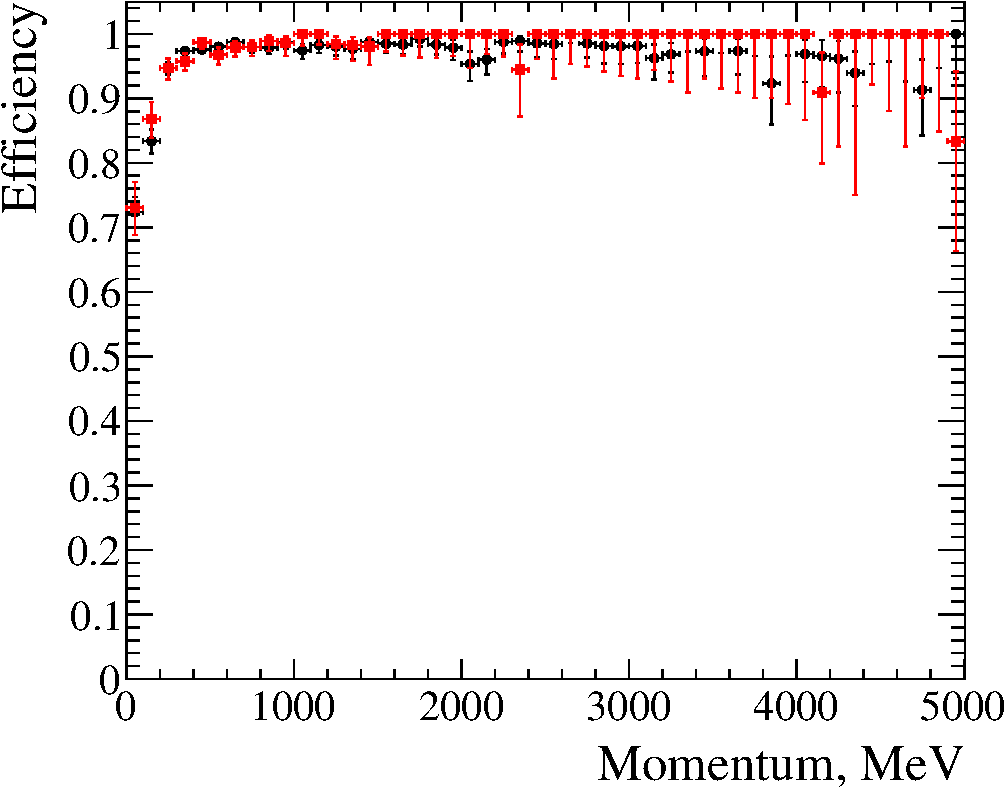
\includegraphics[width=\linewidth]{MomWide}}
    \end{minipage}
    \hfill
    \begin{minipage}[h]{0.49\linewidth}
        \center{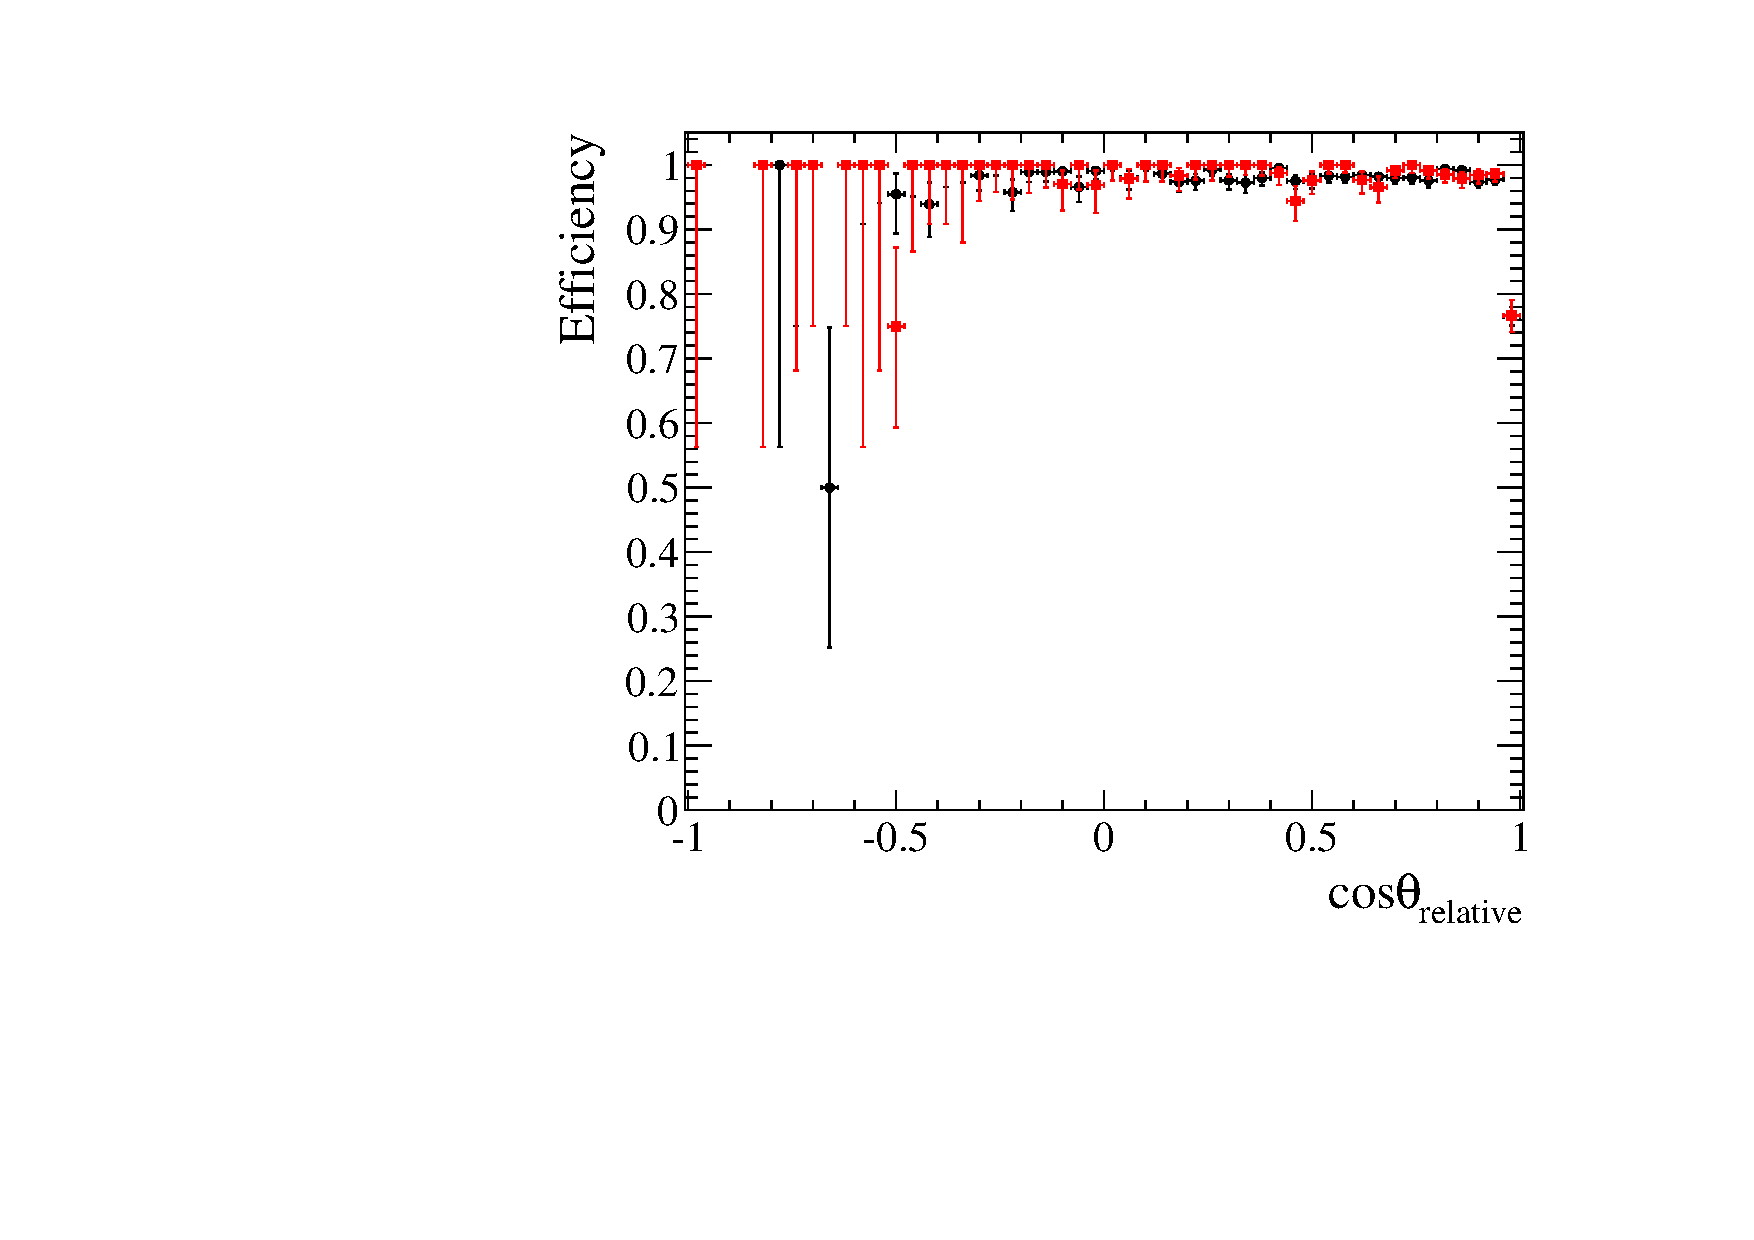
\includegraphics[width=\linewidth]{CosWide}}
    \end{minipage}
    \vfill
    \begin{minipage}[h]{0.49\linewidth}
        \center{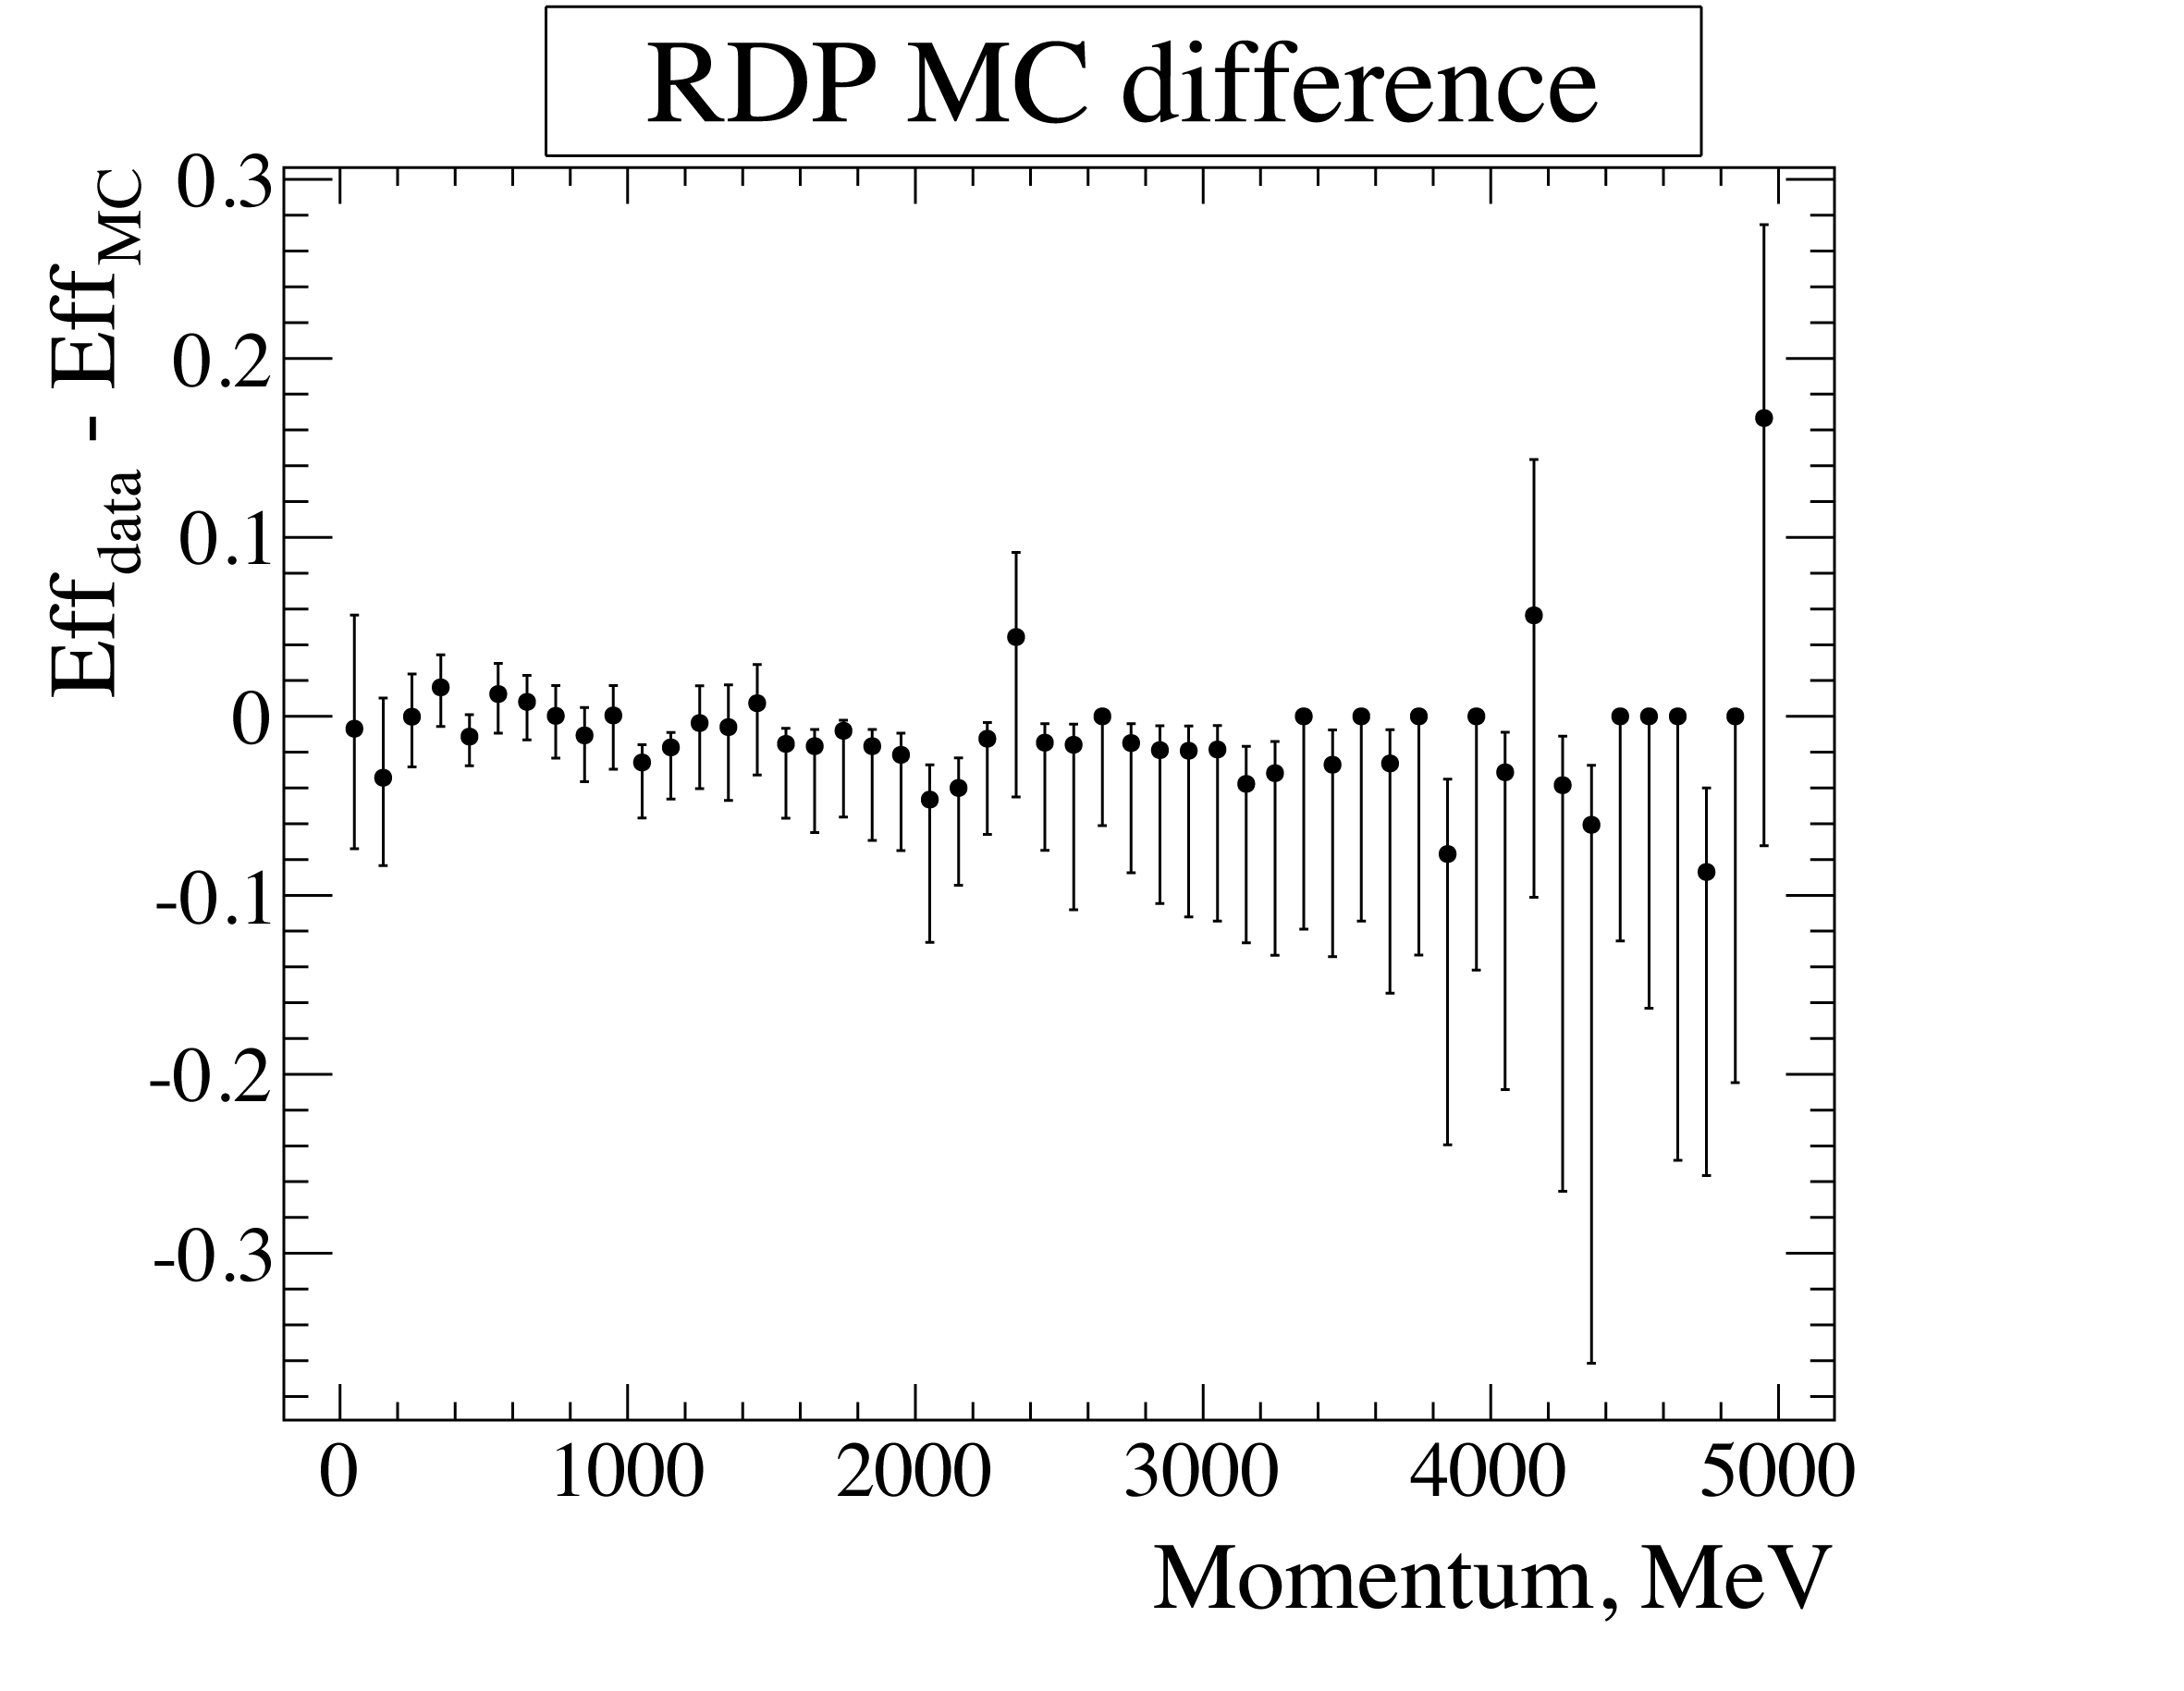
\includegraphics[width=\linewidth]{MomDifWide} \\ a)}
    \end{minipage}
    \hfill
    \begin{minipage}[h]{0.49\linewidth}
        \center{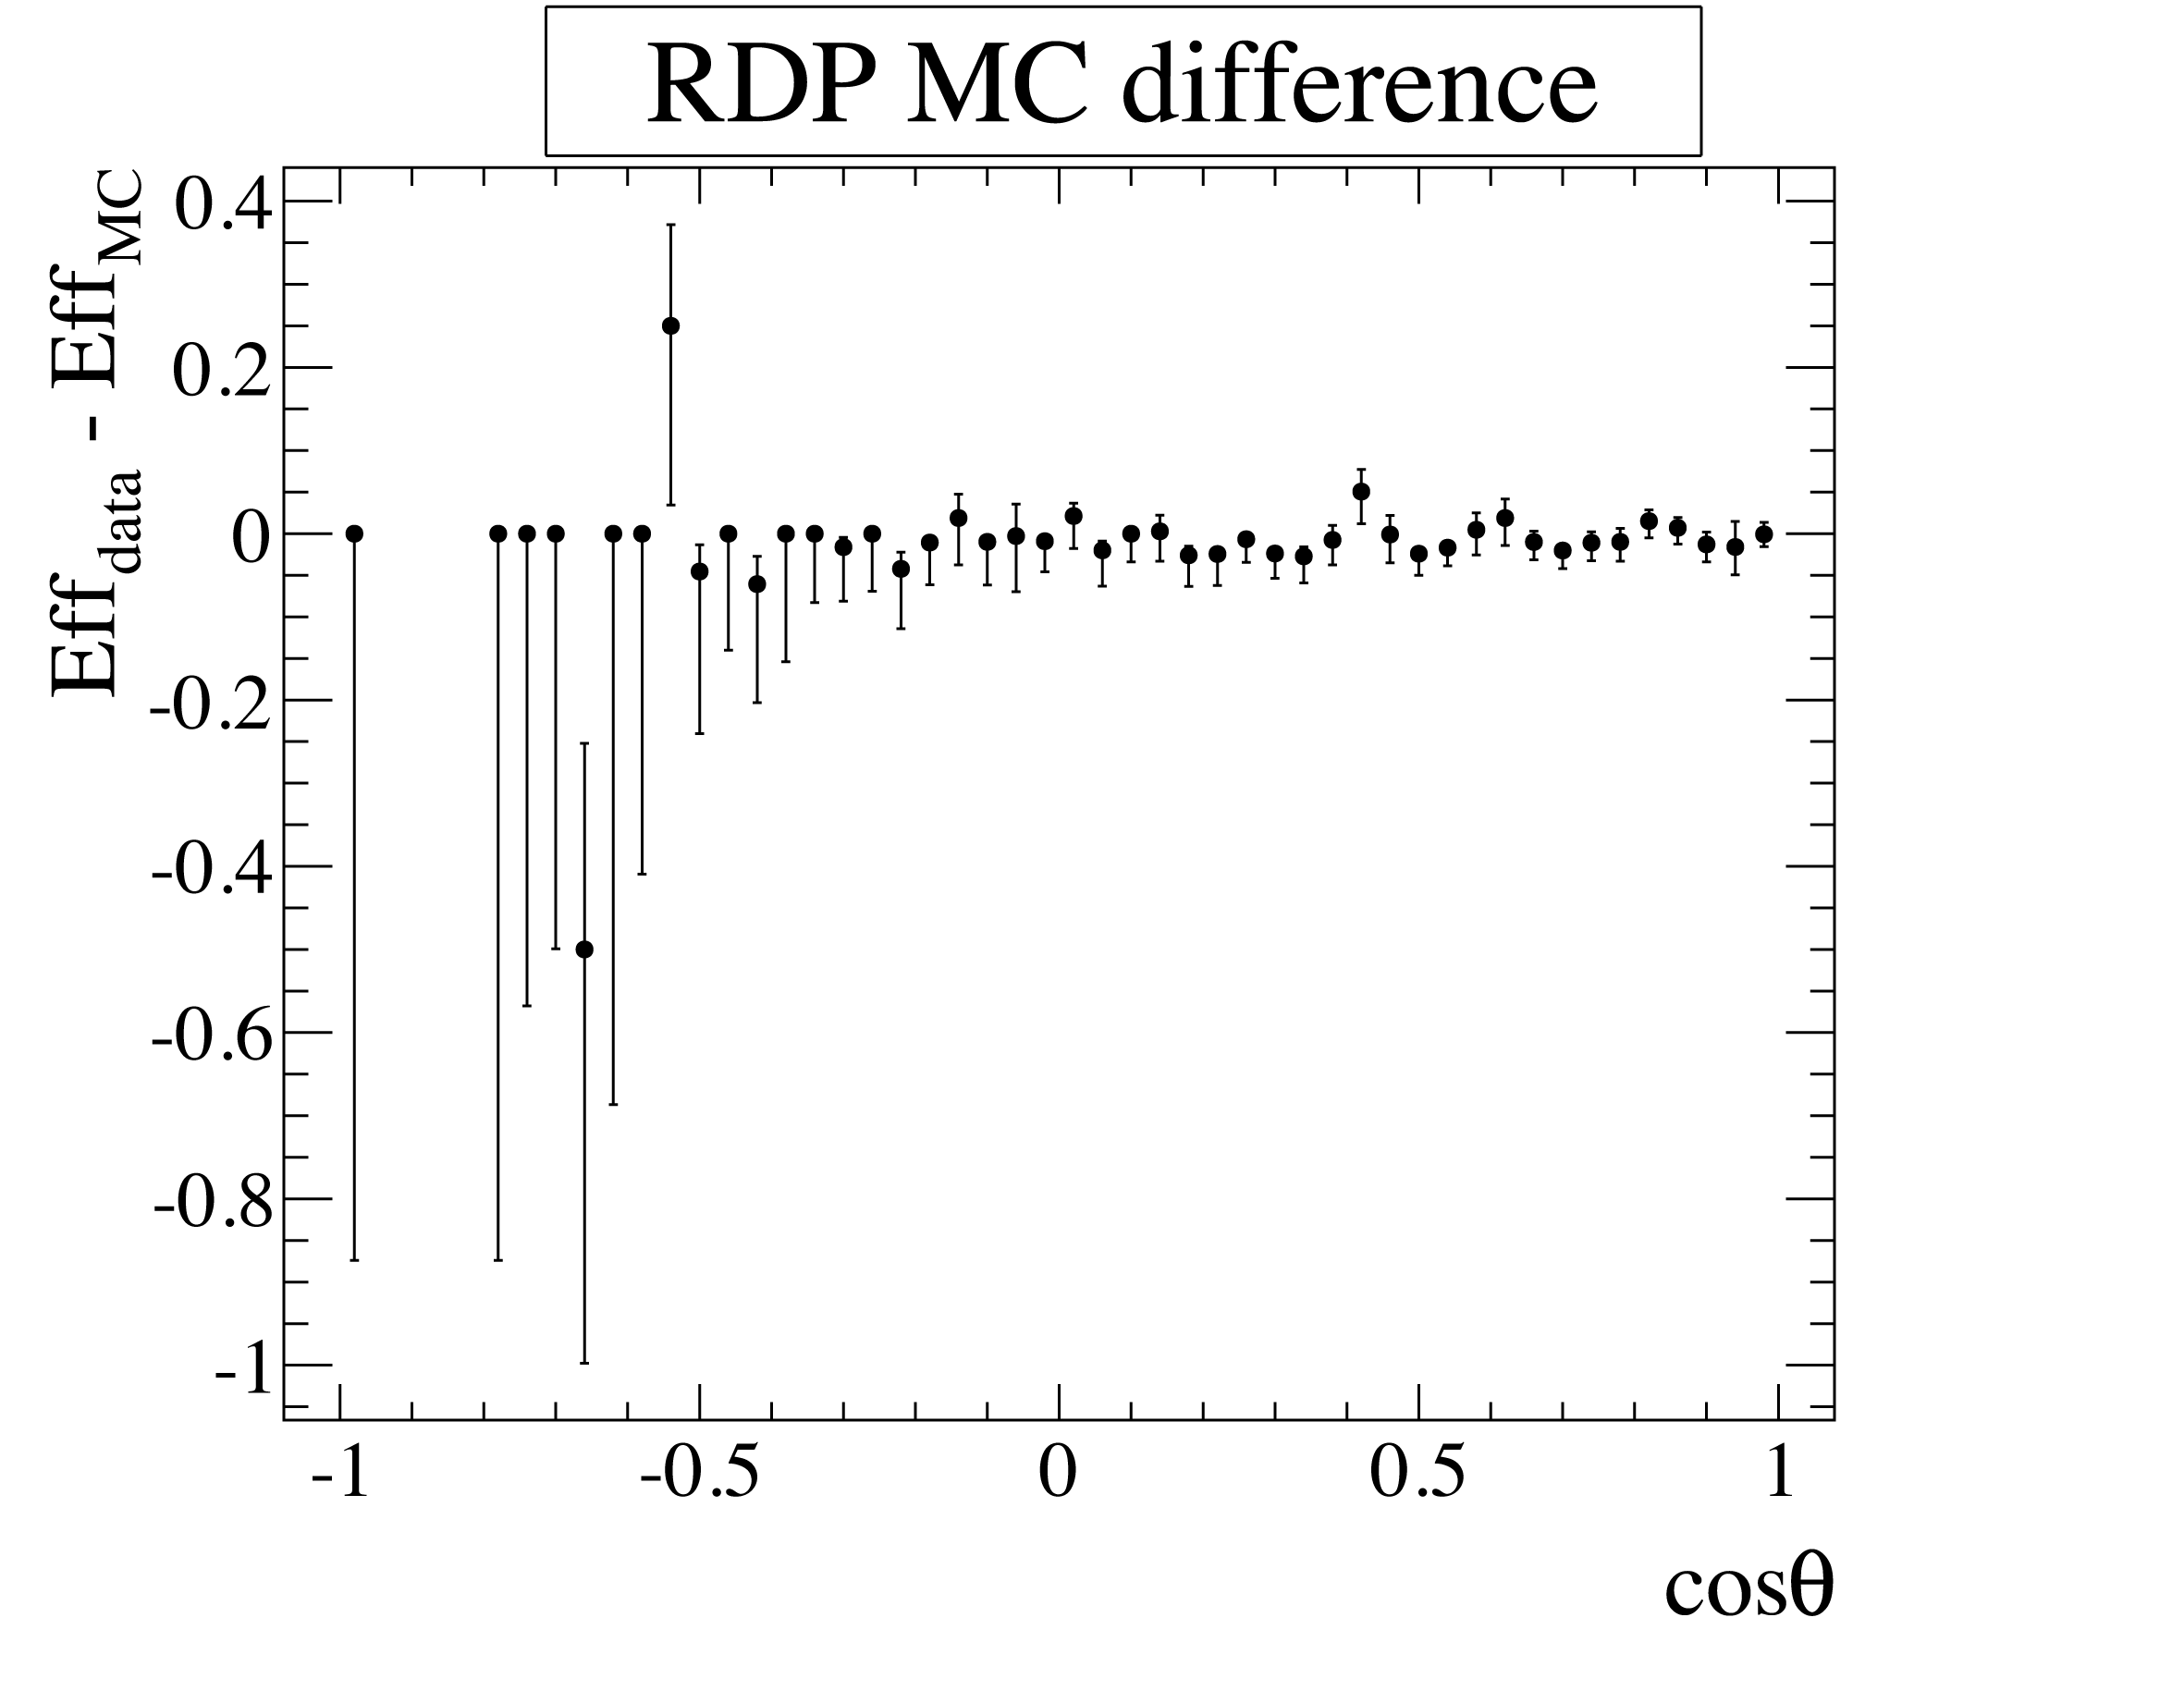
\includegraphics[width=\linewidth]{CosDifWide} \\ b)}
    \end{minipage}
    \caption{Dependence of the global vertex association systematics on the  track momentum (a) and on the opening angle (b) for FGD1 sample in black for DATA and in red for MC.}
    \label{fig:HNL:GVsysDEP}
\end{figure}

I concluded that there is neither angular nor momentum systematics dependence. The efficiency for MC and DATA are presented in \autoref{tbl:HNL:GVsys}. The systematics for the HNL study was estimated using these efficiencies differences with a weight-like method.
\begin{table}[!ht]
\begin{center}
\begin{tabular}{|l|l|l|}
    \hline
    & FGD1 & FGD2 \\
    \hline
    DATA   & $0.958^{+0.0023}_{-0.0024}$ & $0.944^{+0.0027}_{-0.0026}$  \\
    \hline
    MC      & $0.962^{+0.0036}_{-0.0038}$ & $0.952^{+0.004}_{-0.0042}$  \\
    \hline
    Systematic uncertainty for $N\to\mu\pi$ & $0.58\%$ & $0.46\%$ \\
    \hline
    Systematic uncertainty for $N\to e\pi$ & $0.51\%$ & $0.4\%$ \\
    \hline

\end{tabular}
\caption{Global vertex association efficiency and systematics.}
\label{tbl:HNL:GVsys}
\end{center}
\end{table}
One more check is the spatial resolution comparison between the data and MC. We checked the difference between the track start position and the vertex position. The results are shown in \autoref{fig:HNL:res}, the statistics is summarized in \autoref{tbl:HNL:res}. As we can see the mean value for MC and data are rather close, the difference between them is close to the fit error and much less than the statistical uncertainty.
\begin{figure}[!ht]
\begin{center}
    \begin{minipage}{0.49\linewidth}
        \centering{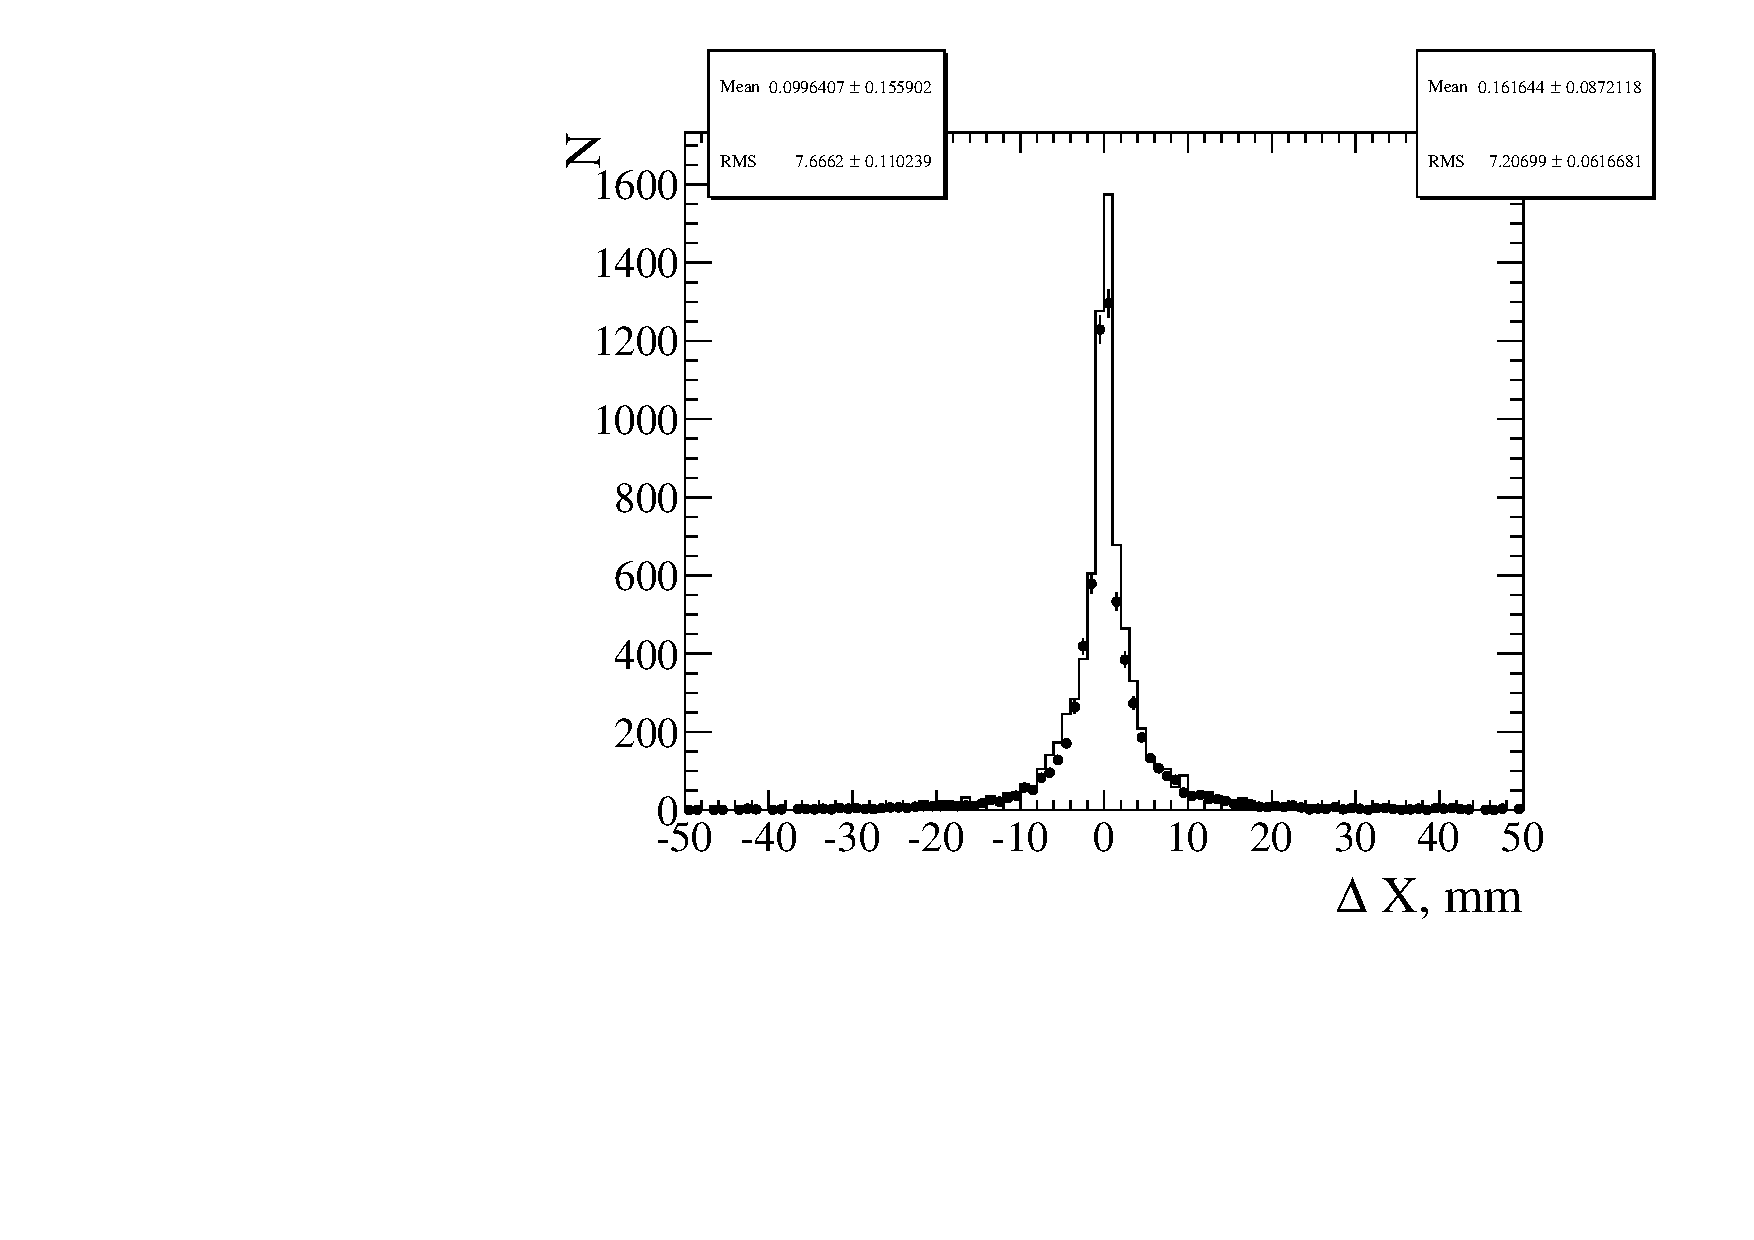
\includegraphics[width=\linewidth]{ResolutionX}}
    \end{minipage}
    \hfill
    \begin{minipage}{0.49\linewidth}
        \centering{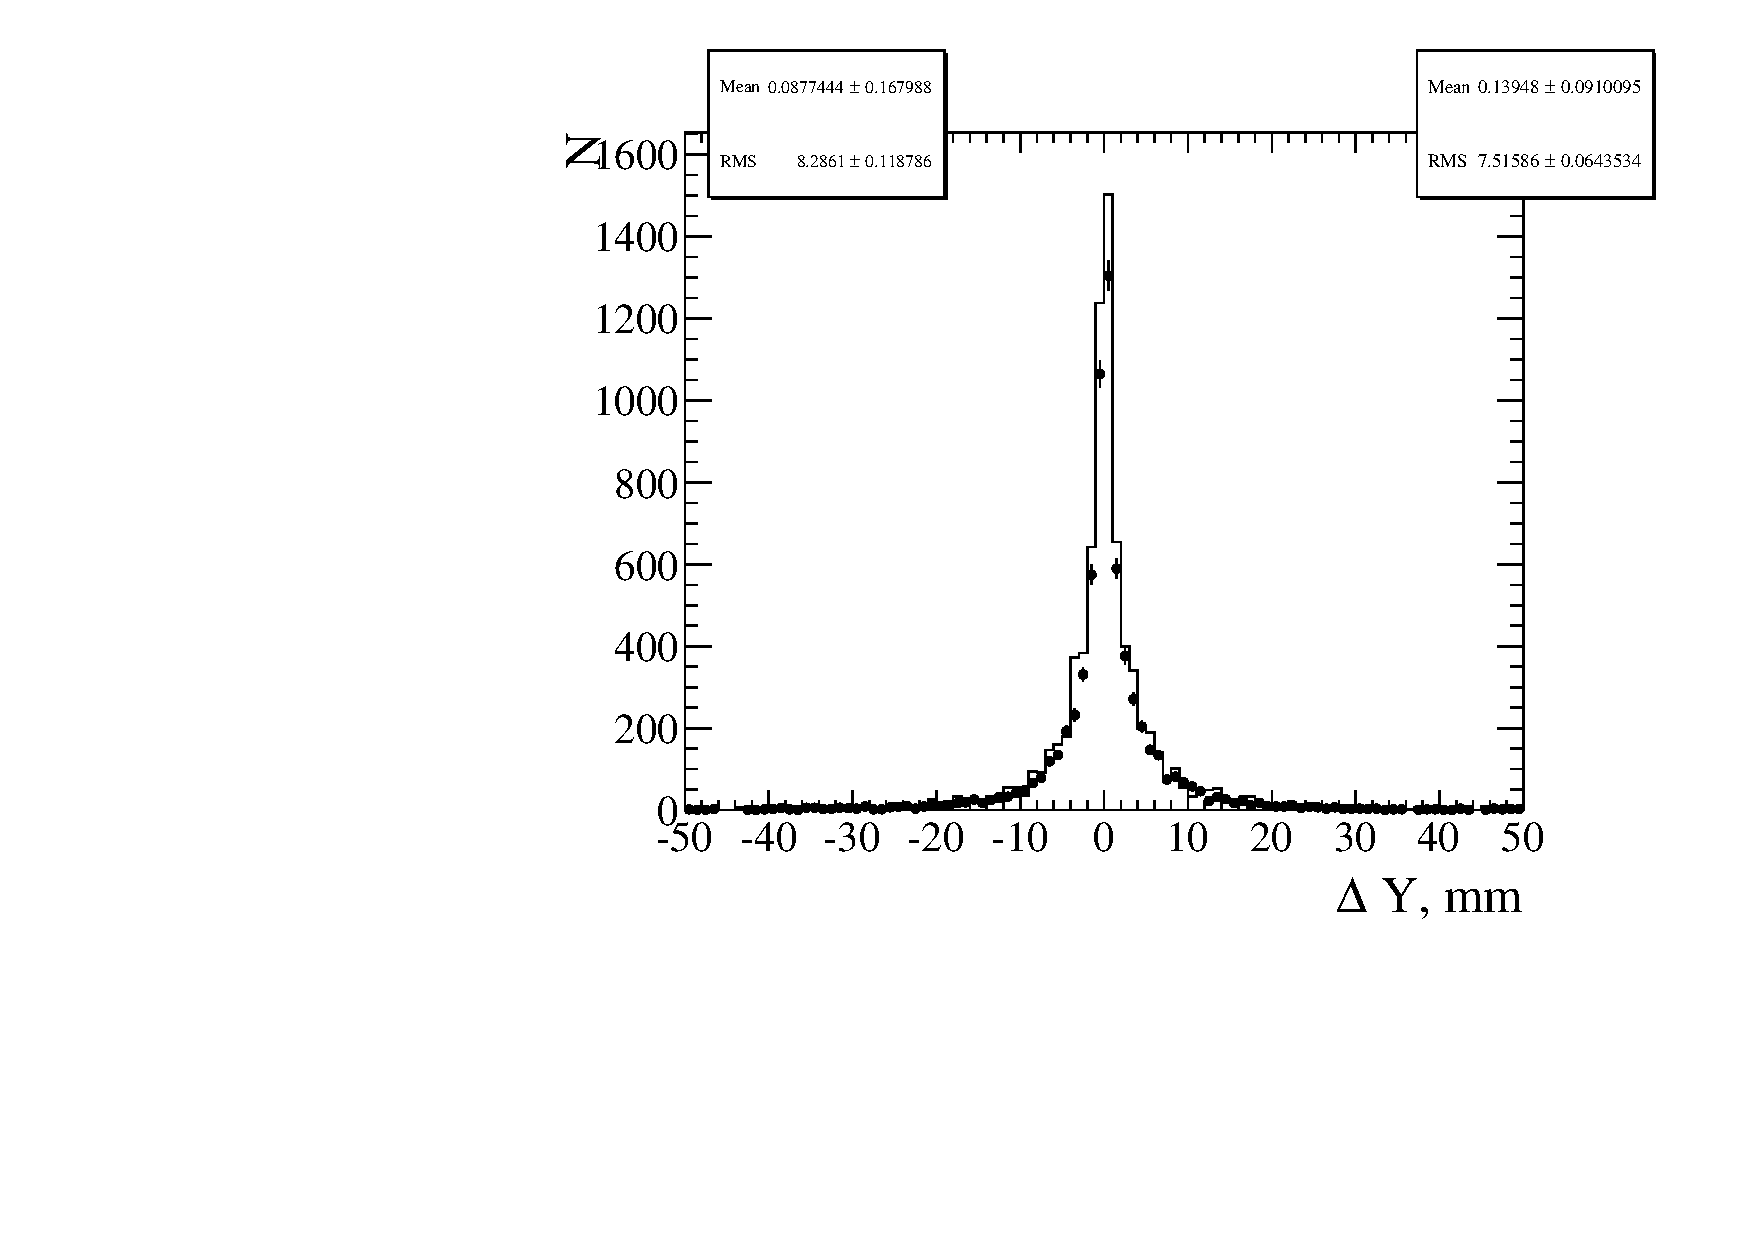
\includegraphics[width=\linewidth]{ResolutionY}}
    \end{minipage}
    \vfill
    \begin{minipage}{0.49\linewidth}
        \centering{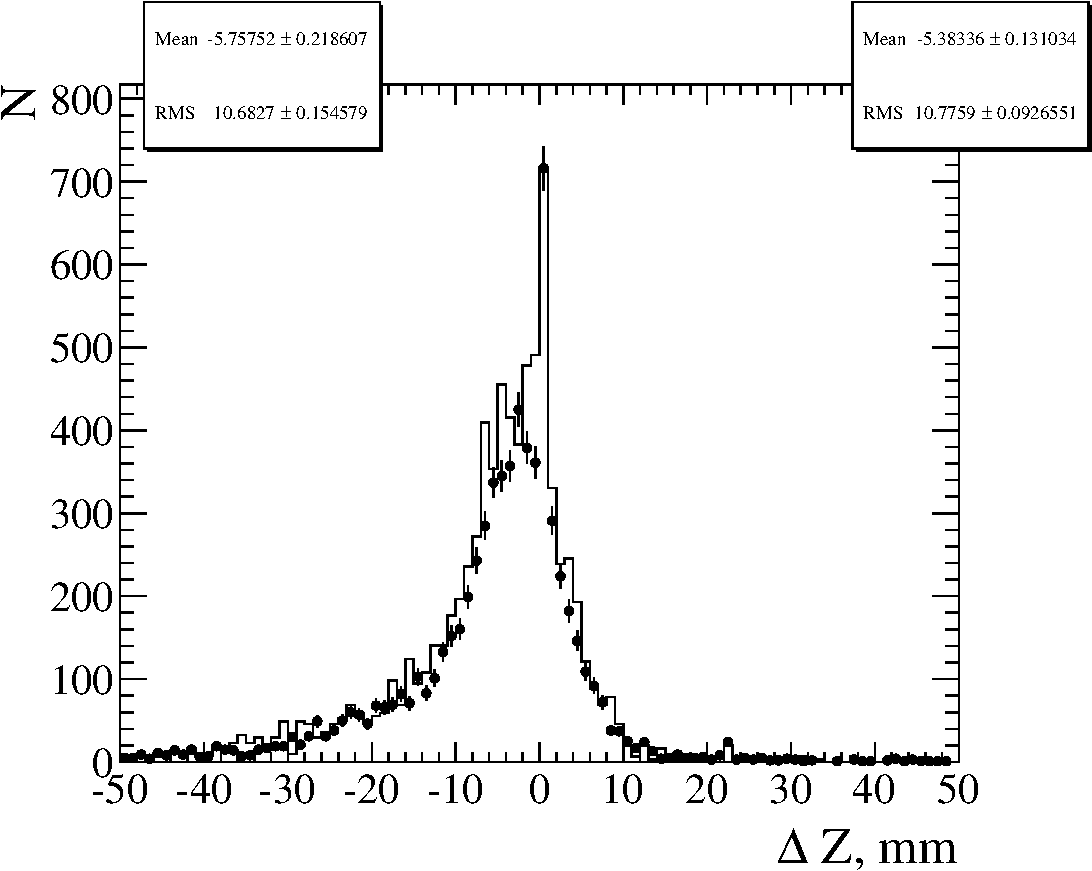
\includegraphics[width=\linewidth]{ResolutionZ}}
    \end{minipage}
    \caption{Global vertex spatial resolution for experimental and MC data. Dots and left statistic box corresponds to experimental data, histograms and right statistic represents the simulation result.}
    \label{fig:HNL:res}
\end{center}
\end{figure}

\begin{table}[!ht]
\begin{center}
\begin{tabular}{|c|c|c|c|}
    \hline
    Axis & & Mean & RMS \\
    \hline
    \multirow{2}{*}{X} & MC & $0.16 \pm 0.09$ & $7.20\pm0.06$\\

    & DATA & $0.1\pm0.16$ & $7.67\pm0.11$ \\
    \hline
    \multirow{2}{*}{Y} & MC & $0.09 \pm 0.17$ & $8.29 \pm 0.12$\\

    & DATA & $0.14 \pm 0.09$ & $7.5 \pm 0.06$ \\
    \hline
    \multirow{2}{*}{Z} & MC & $-5.76 \pm 0.22$ & $10.68 \pm 0.15$\\

    & DATA & $-5.38 \pm 0.13$ & $10.78 \pm 0.09$ \\
    \hline
\end{tabular}
\caption{Summary of the statistics for spatial resolution for experimental and MC data presented in \autoref{fig:HNL:res}.}
\label{tbl:HNL:res}
\end{center}
\end{table}

\begin{comment}
The results of all the systematic study are presented in \autoref{tab:HNL:sys}.
\begin{table}[!ht]
\begin{center}
\begin{tabular}{|l |c| c| c|}
  \hline
   & $\mu\pi$ & $e\pi$ & $\mu\mu\nu$\\
  \hline
  \multicolumn{4}{||l|}{Variation-like} \\
  \hline
  B Field distortions                 & 0.48\%    & 0.37\%         &  0.02\%\\
  TPC momentum scale                  & 0.03\%    & 0.01\%         & 0.04\%\\
  TPC momentum resolution             & 2.34\%    & 0.78\%         & 0.46\%\\
  TPC PID                             & 0.41\%    & 0.75\%         & 1\%\\
  \hline
  \multicolumn{4}{||l|}{Efficiency-like} \\
  \hline
  TPC cluster efficiency              &   $\ll1\%$   &   $\ll1\%$  &  0.01\%\\
  TPC tracking efficiency             &   0.44\%     &  0.34 \%    & 0.46\% \\
  TPC charge ID efficiency            &   0.04\%     &   0.21\%    &   0.76\%\\
  TPC-FGD matching                    &   0.27\%     &    $\ll1\%$ & 0.03\%\\
  Pion secondary interactions         &   3.88\%     &   2.91\%    &  - \\
  Global vertex combining             &    0.58\%    &  0.52\%     & 0.48\%\\
  ECal PID                            &     -        &     -       & 0.27\%\\
  ECal TPC matching                   &     -        &     -       &  0.01\%\\
  \hline
  Total                               &   4.64\%     &  3.20\%     & 1.51\%\\
  \hline
\end{tabular}
\caption{Detector systematics summary.}
\label{tab:HNL:sys}
\end{center}
\end{table}
\end{comment}

The detector systematic dependence on HNL mass is shown in \autoref{fig:HNL:sys} and \autoref{fig:HNL:sysDimuon}. As one can see the most critical uncertainty comes from the pion secondary interactions for the modes $e\pi$ and $\mu\pi$. As the dimuon mode $\mu\mu\nu$ doesn't produce pions in the final state it's free from that uncertainty and the total error is much smaller.

\begin{figure}[!ht]
  \begin{minipage}{0.49\linewidth}
    \centering{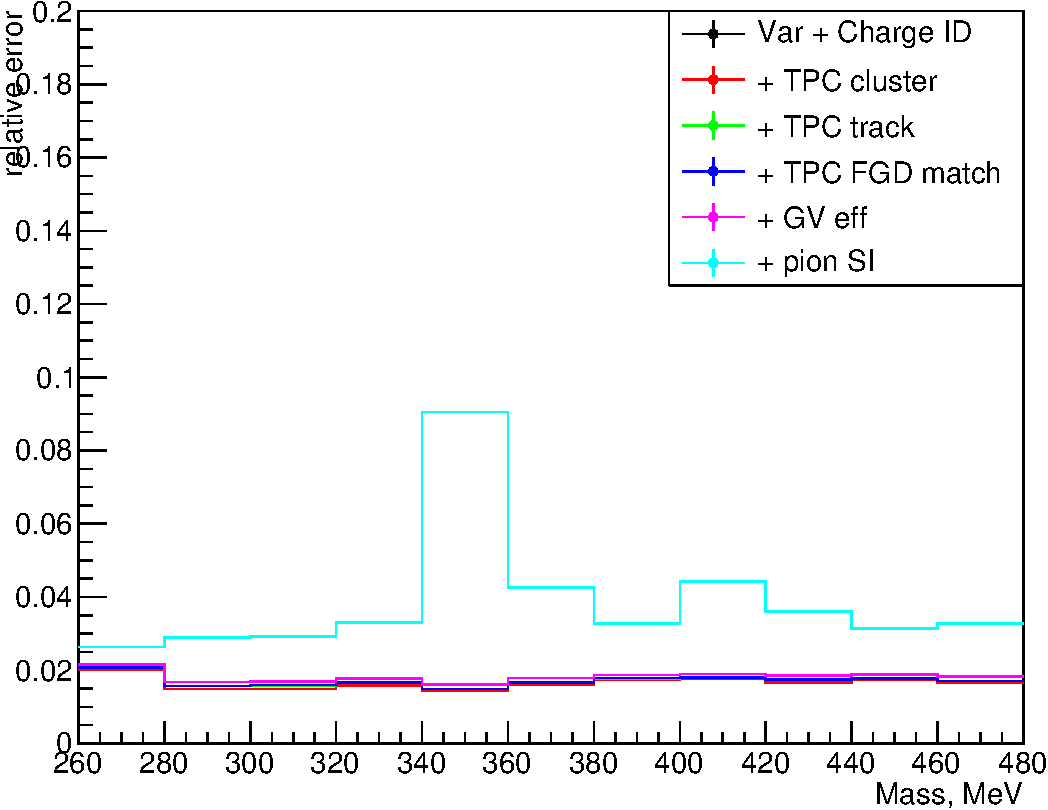
\includegraphics[width=\linewidth]{MuPiSys} \\ $K^+\to e^+N\to e^+\left(\mu^-\pi^+\right)$}
  \end{minipage}
  \begin{minipage}{0.49\linewidth}
    \centering{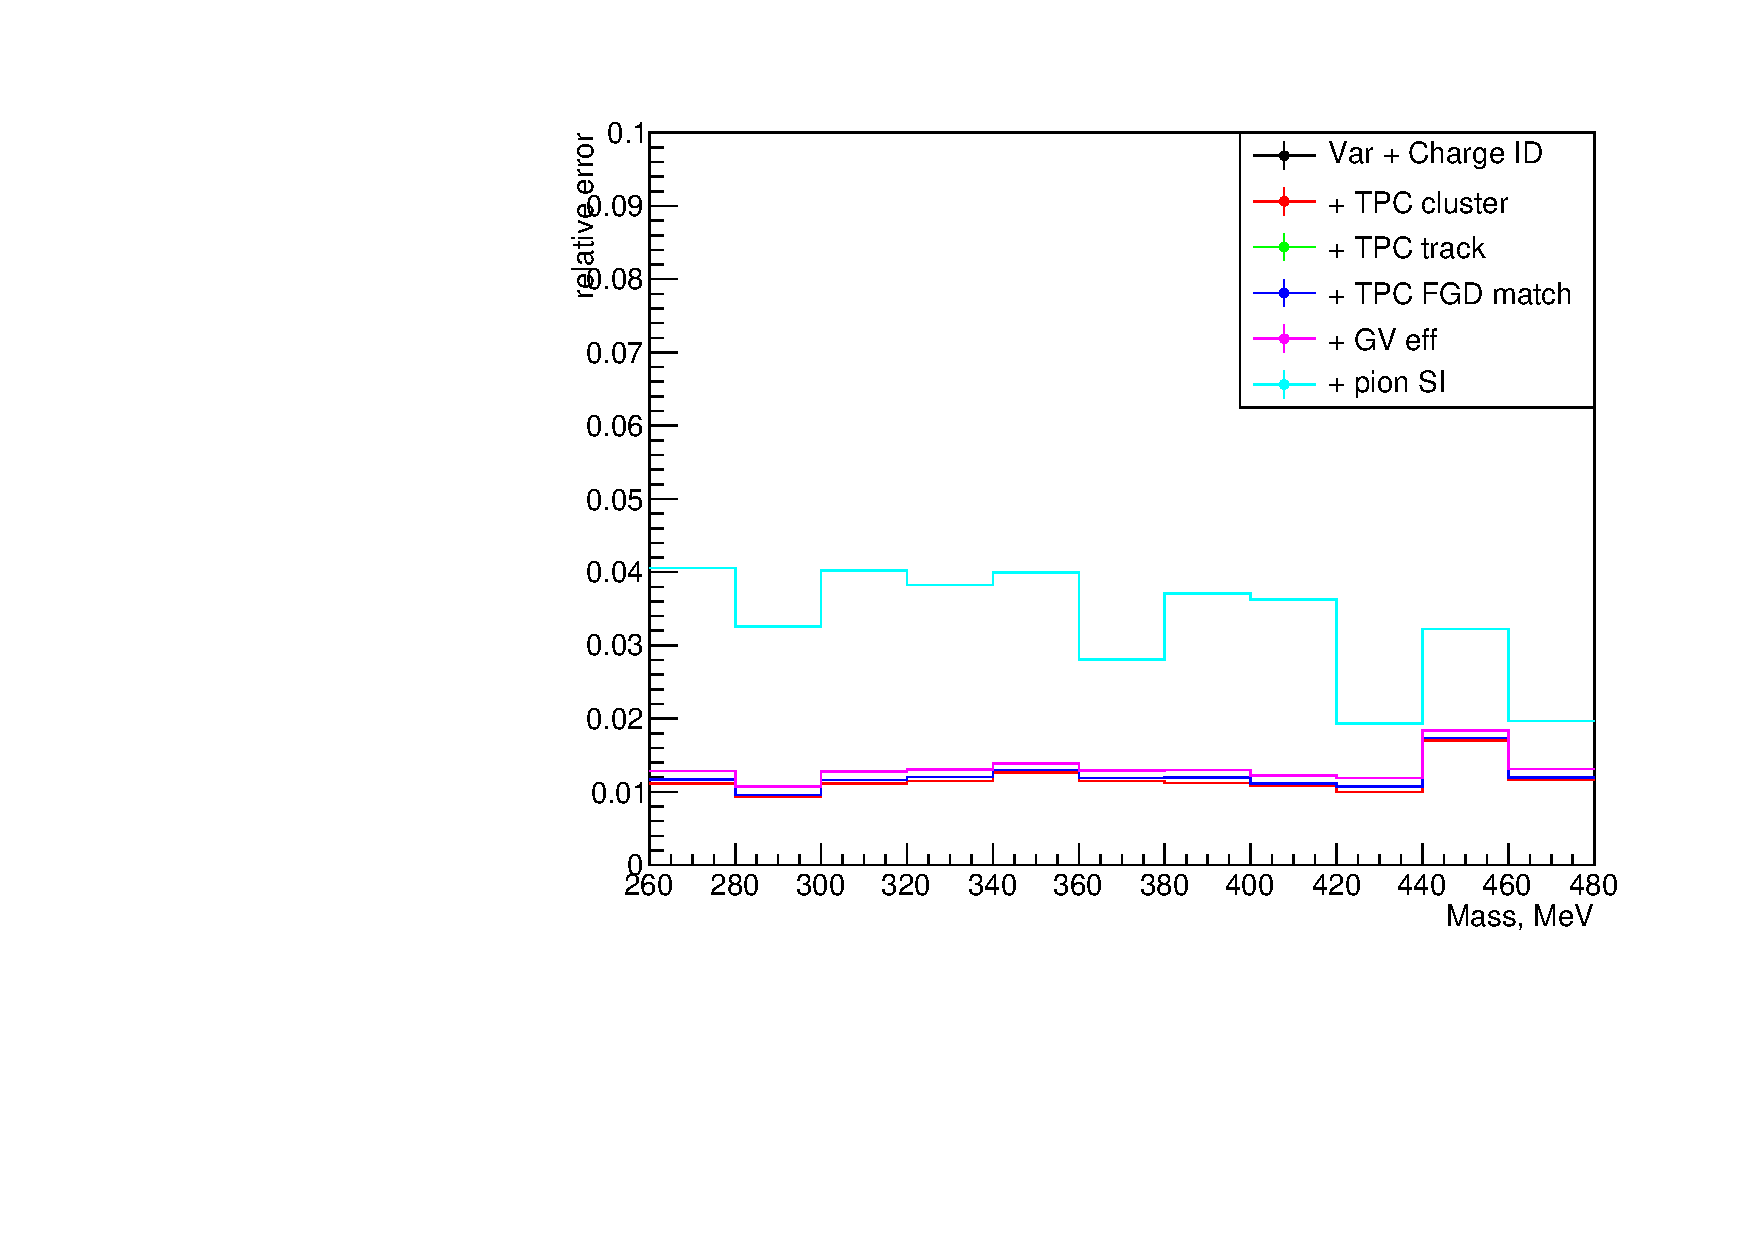
\includegraphics[width=\linewidth]{ElePiSys} \\ $K^+\to e^+N\to e^+\left(e^-\pi^+\right)$}
  \end{minipage}
  \caption{Detector systematics dependence on HNL mass}.
  \label{fig:HNL:sys}
\end{figure}

\begin{figure}[!ht]
    \centering{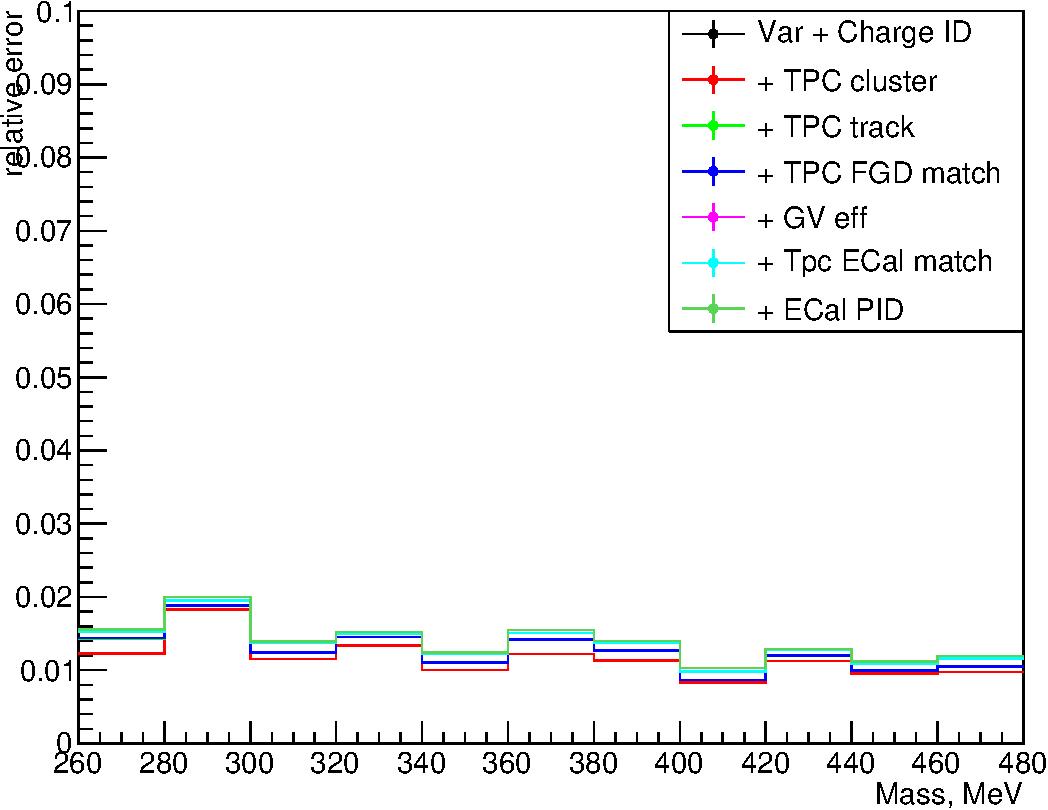
\includegraphics[width=0.49\linewidth]{DiMuonSys} \\ $K^+\to e^+N\to e^+\left(\mu^-\mu^+\nu\right)$}
  \caption{Detector systematics dependence on HNL mass}.
  \label{fig:HNL:sysDimuon}
\end{figure}


\subsection{Flux systematics}

Heavy neutrino flux in the ND280 is calculated based on the kaon flux produced in the proton collisions. Thus uncertainties of the kaon flux will affect the number of signal events. The total flux error consists of the uncertainties of the meson multiplicities, pion re-scatter, interaction length, focusing and other errors~\cite{Abe2013}. These fractional errors and the total flux uncertainty for the active neutrino beam are presented in the \autoref{fig:HNL:FluxError}. To estimate the kaon multiplicity errors we use data from NA61/SHINE. Relative uncertainties of the kaon multiplicities are shown in \autoref{fig:HNL:KaonMult}. For HNL analysis we deal mainly with the kaons collinear to the beam axis. We consider a conservative estimation of the kaon multiplicity uncertainty as 20\%. For all the other sources of the flux errors, we take the maximum value among all energy bins.

\begin{figure}[!ht]
\begin{minipage}{0.49\linewidth}
  \centering{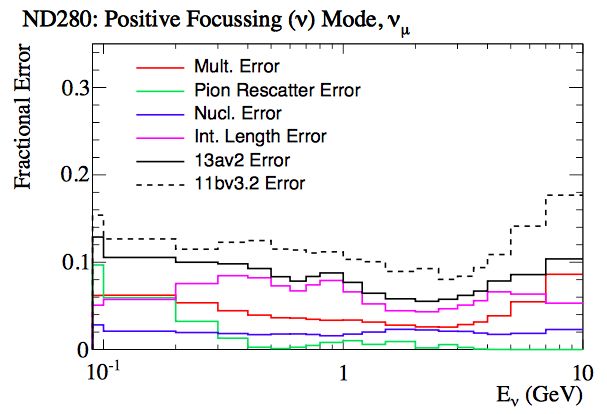
\includegraphics[width=\linewidth]{NuFluxError.png} }
  \caption{$\nu_\mu$ Flux uncertainties.}
  \label{fig:HNL:FluxError}
\end{minipage}
\hfill
\begin{minipage}{0.49\linewidth}
  \centering{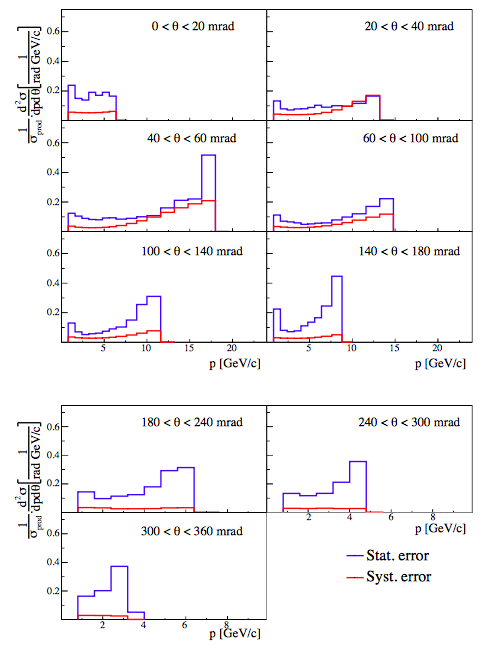
\includegraphics[width=0.49\linewidth]{KaonError.png} }
  \caption{Kaon multiplicity uncertainties.}
  \label{fig:HNL:KaonMult}
\end{minipage}
\end{figure}

The results of the systematics study are presented in the \autoref{fig:HNL:AllSys}. The detector systematics is widely described in the previous subsection. As we analyze all charge conjugated modes together we take the highest systematics uncertainties among them.

\begin{figure}[!ht]
    \begin{center}
    \begin{minipage}{0.49\linewidth}
        \centering{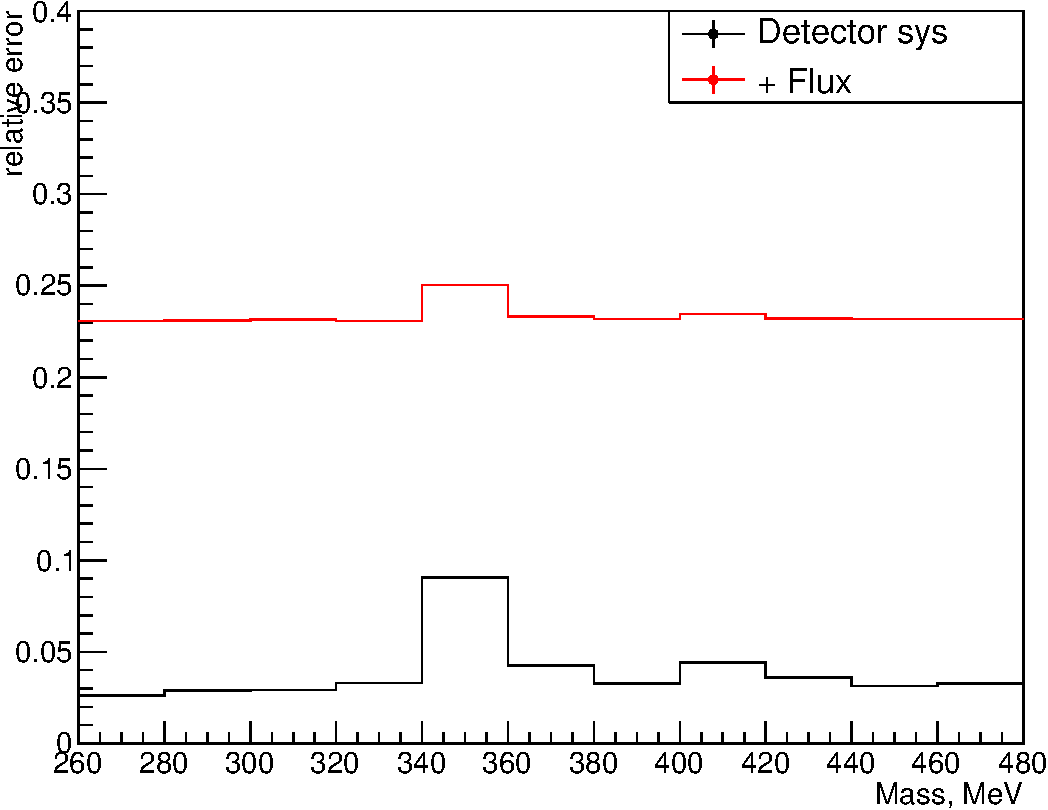
\includegraphics[width=\linewidth]{FluxMu}  \\  $N\to\mu\pi$}
    \end{minipage}
    \hfill
    \begin{minipage}{0.49\linewidth}
        \centering{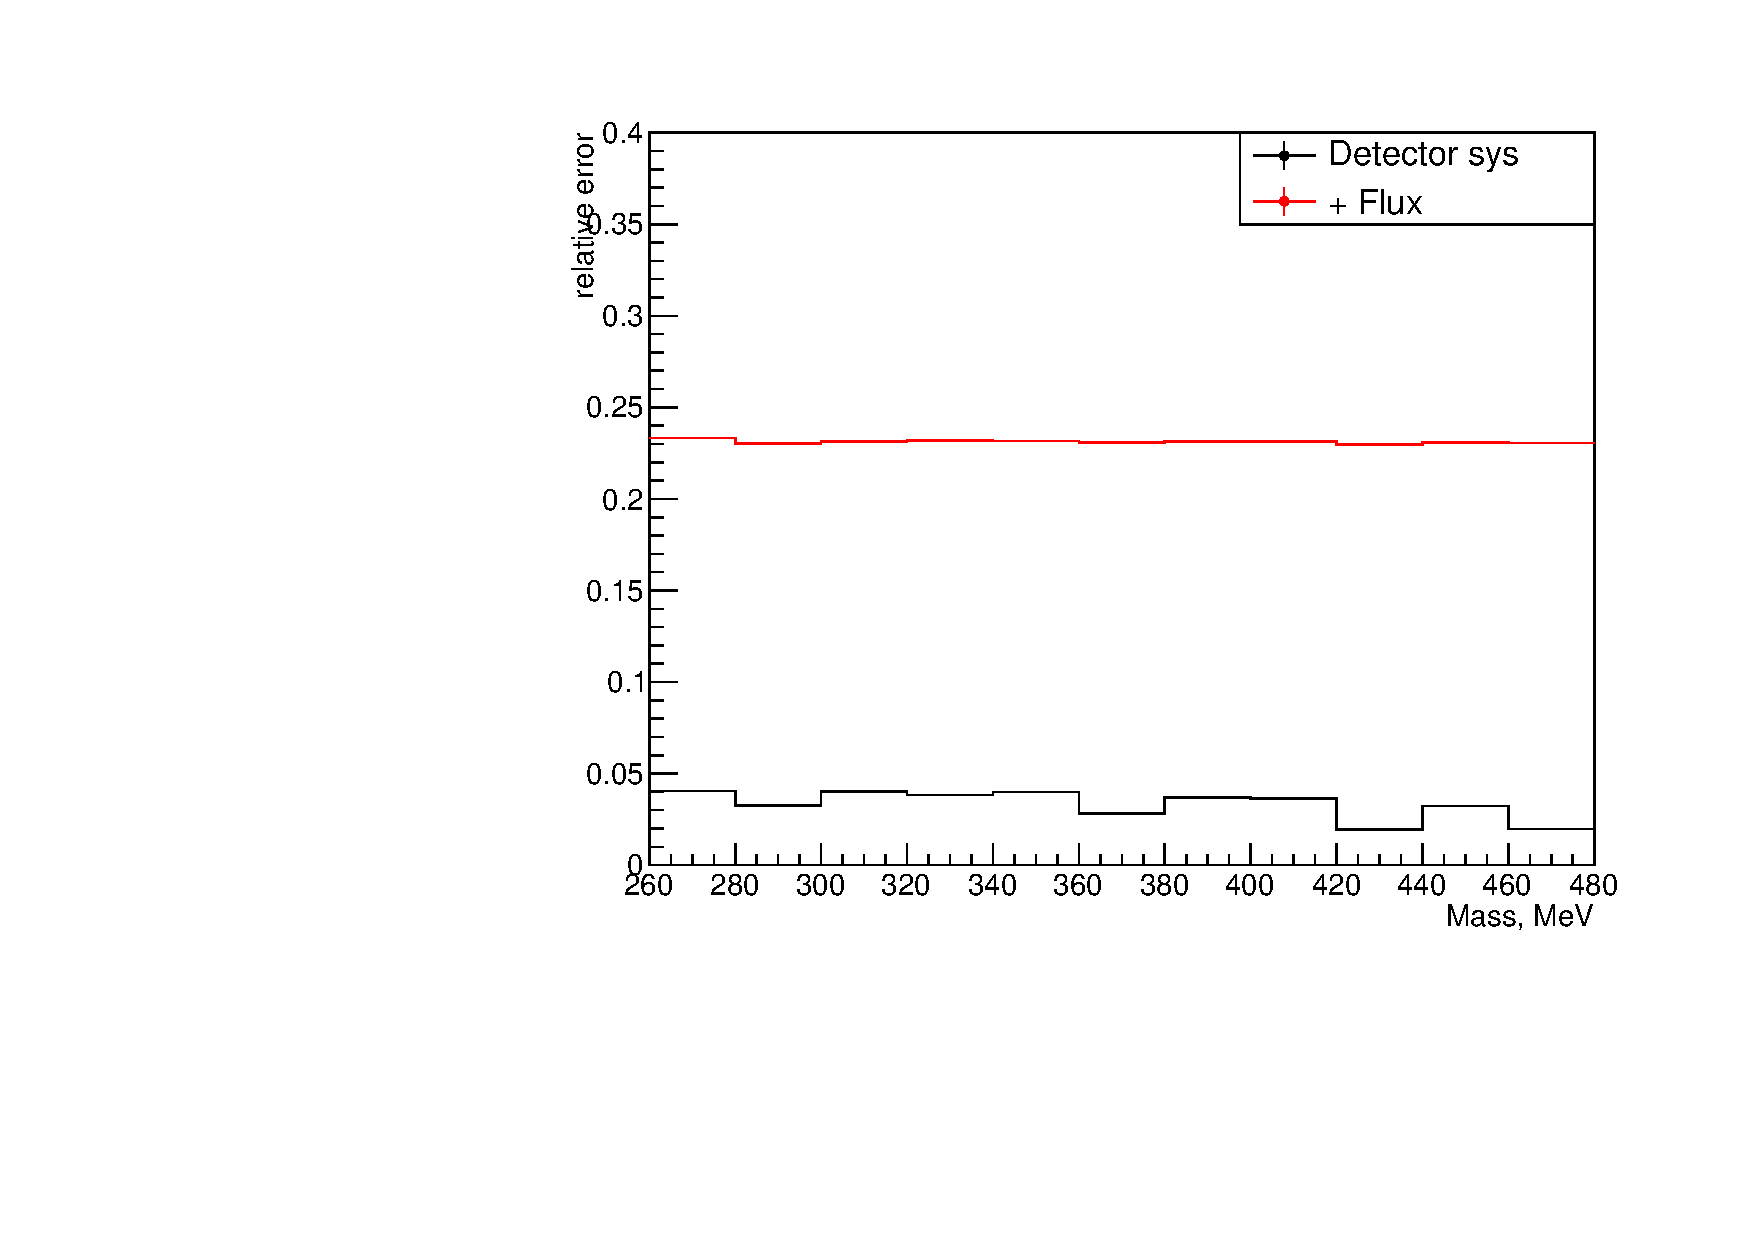
\includegraphics[width=\linewidth]{FluxEle}  \\  $N\to e\pi$}
    \end{minipage}
    \vfill
    \begin{minipage}{0.49\linewidth}
        \centering{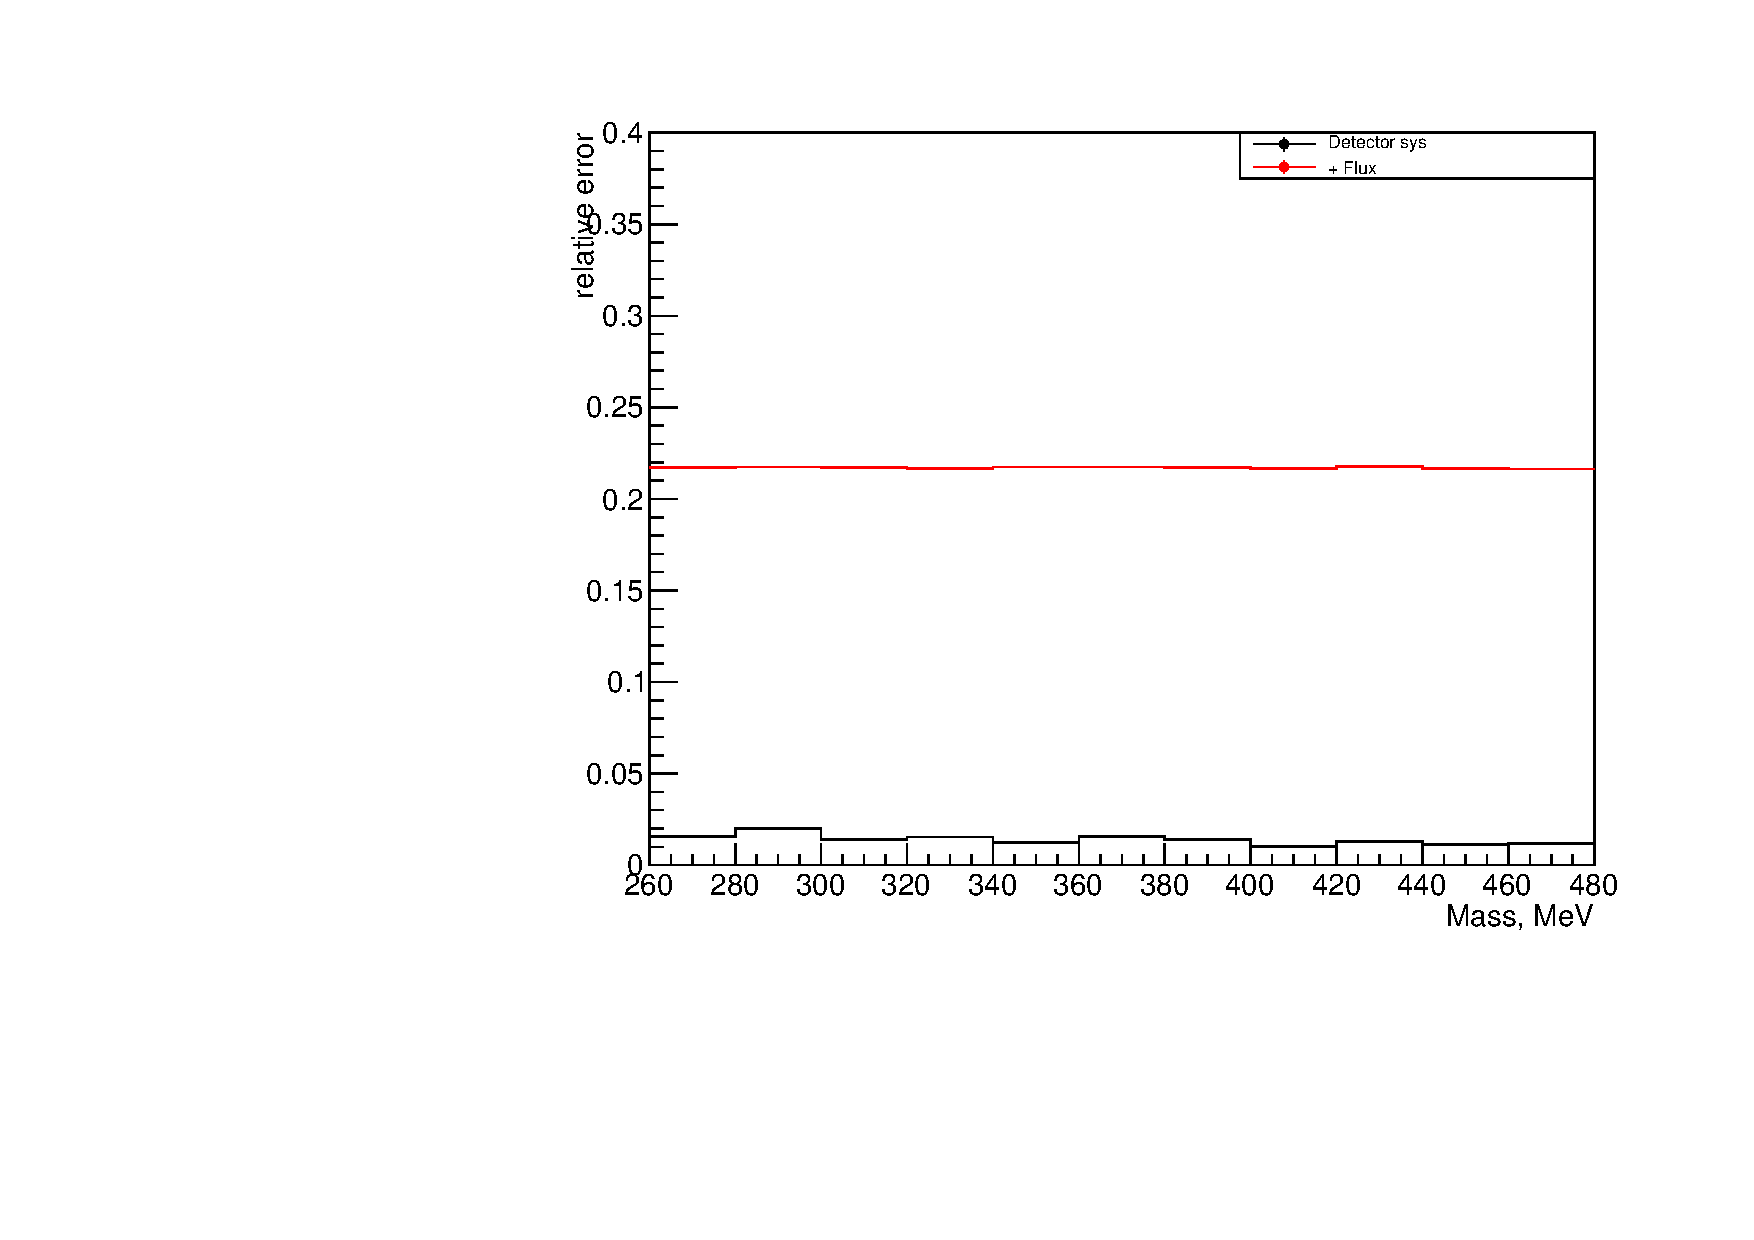
\includegraphics[width=\linewidth]{FluxDiMu}  \\  $N\to\mu\mu\nu$}
    \end{minipage}
    \caption{Detector and flux systematic errors for different modes.}
    \label{fig:HNL:AllSys}
        \end{center}
\end{figure}

\section{Statistical methods}
\label{sec:HNL:stat}
The statistical approach to the low-level signal analysis is described in the Highland and Cousins work~\cite{Cousins1992}. As the number of the HNL decay events is proportional to the fourth power of the mixing element, constraints on $\left|U_i\right|^2$ without systematics looks like:
\begin{equation}
  \left|U_i\right|^2_{limit}=\sqrt{\frac{U_n}{N_{events}}}
  \label{eq:HNL:constraints}
\end{equation}
where
\begin{itemize}
    \item $i=e,\mu$ is a lepton flavor,
    \item $U_n$ is 90\% C.L. Poisson limit for $n$ observed events,
    \item $N_{events}$ is an expected number of signal events assuming $\left|U\right|^2=1$.
\end{itemize}
If we take into account the detector acceptance uncertainty, the result can be calculated according to~\cite{Cousins1992}:
\begin{equation}
  U_n=U_{n0}\left\{1+E_n\frac{\sigma^2_{Acc}}{2}\left(1+\left(\frac{E_n\sigma_{Acc}}{2}\right)^2\right)\right\}
  \label{eq:HNL:constrainsAcc}
\end{equation}
where
\begin{itemize}
    \item $U_{n0}$ is 90\% C.L. Poisson limit for $n$ observed events,
    \item $\sigma_{Acc}$ is the acceptance error,
    \item $E_n=U_{n0}-n$ represents the excess of the upper limit of a Poisson parameter over the number n of observed events, for a specified confidence level.
\end{itemize}
This approach can be applied only while $\sigma_{Acc}<1/E_n$. We already showed that in our study $\sigma_{Acc}\approx0.3$ and $1/E_n>0.5$ (\autoref{sec:HNL:sys}). So this method can be applied for the analysis.

One more important feature of the current analysis is that we don't consider the background and its uncertainty. We used the background estimations to tune our selection. For the final result we will treat all the observed events as a signal and then put a conservative limit on the mixing elements. The data--driven approach will be indeed conservative, but the advantage is that we are free from the background uncertainty at all. If during the unblinding several events were found we would put the worse limits on the mixing. Such a method can be improved in the future (see \autoref{sec:HNL:prosp}).

\section{Results}
\subsection{MC sensitivity estimations}
\label{sec:HNL:MCres}

After studying the MC efficiency (\autoref{sec:HNL:eff}), background processes (\autoref{sec:HNL:bg}) and systematics (\autoref{sec:HNL:sys}),  sensitivity to the mixing elements based on MC can be estimated according to \autoref{eq:HNL:constrainsAcc}. Because of the small background the acceptance uncertainties have a small effect on the sensitivity.

\begin{comment}
\begin{figure}[!ht]
    \begin{center}
  \begin{minipage}{0.49\linewidth}
    \centering{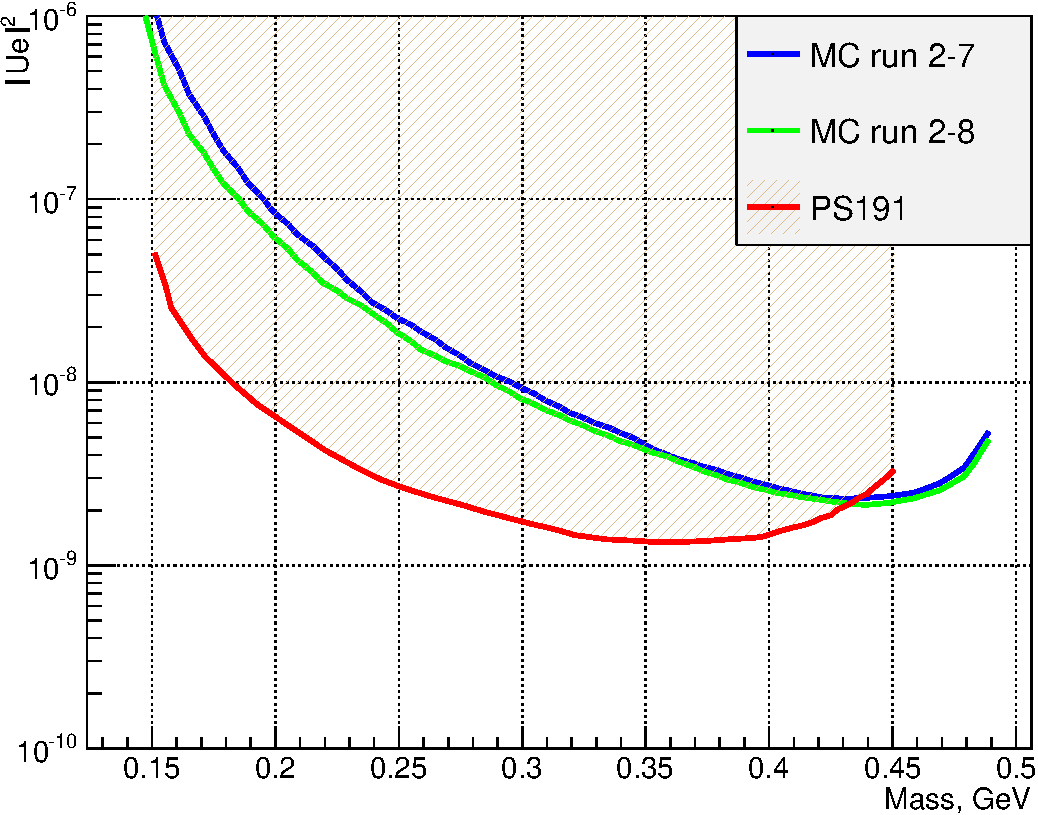
\includegraphics[width=\linewidth]{Ue2fullMC}  \\  $K^+\to e(e\pi)$}
  \end{minipage}
  \hfill
  \begin{minipage}{0.49\linewidth}
    \centering{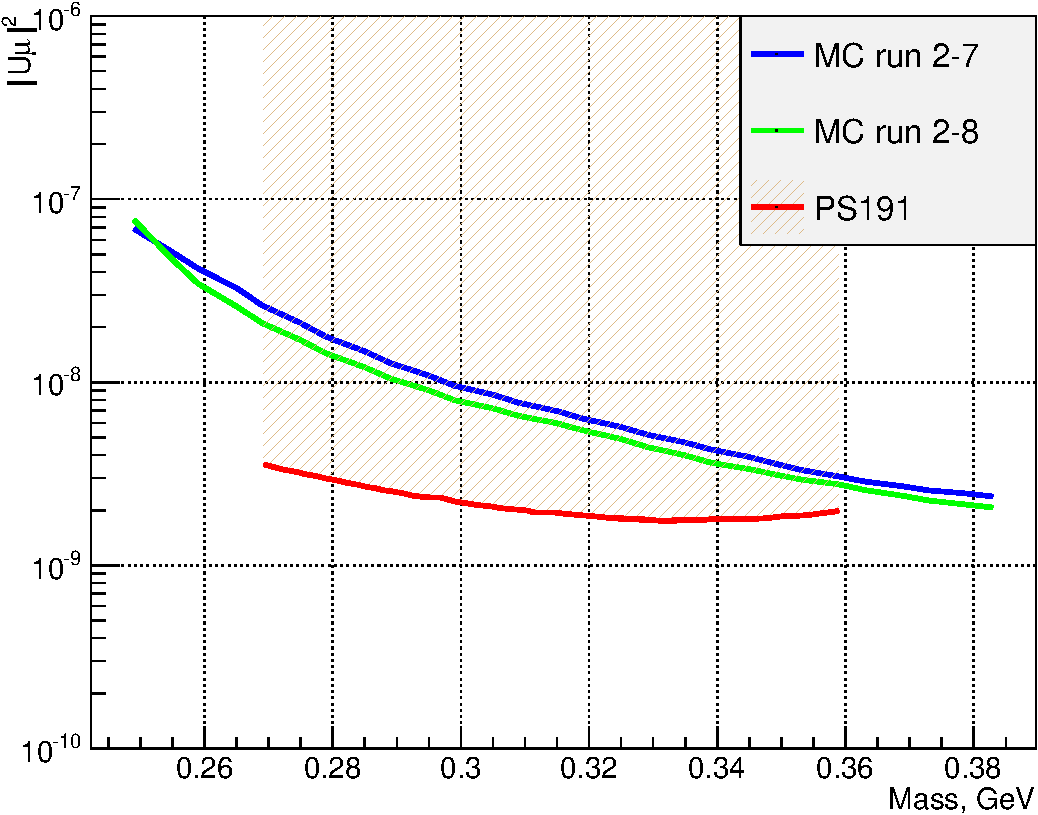
\includegraphics[width=\linewidth]{Umu2fullMC}  \\  $K^+\to \mu(\mu\pi)$}
  \end{minipage}
  \caption{Sensitivity to mixing elements $\left|Ue\right|^2, \left|U\mu\right|^2$ based on MC samples analysis}
  \label{fig:HNL:LimitsMC1}
    \end{center}
\end{figure}

\begin{figure}[!ht]
    \begin{center}
  \begin{minipage}{0.49\linewidth}
    \centering{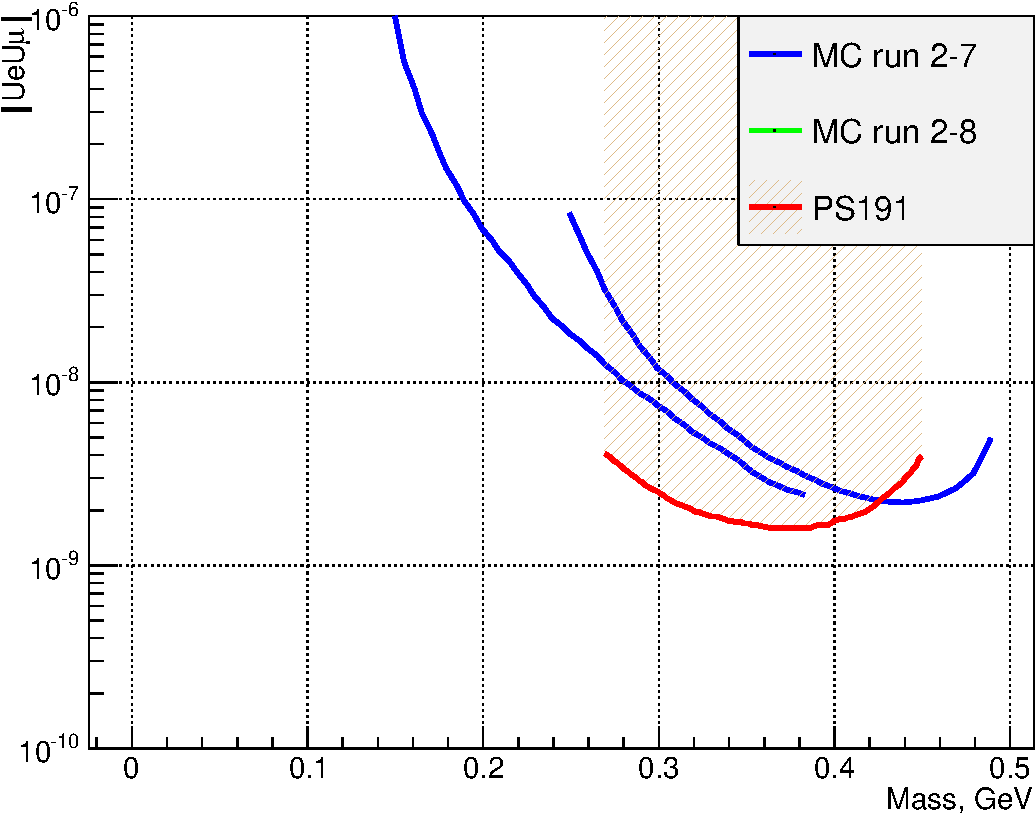
\includegraphics[width=\linewidth]{UeUmufullMC}  \\  $K^+\to \mu(e\pi)$ and $K^+\to e(\mu\pi)$}
  \end{minipage}
  \begin{minipage}{0.49\linewidth}
    \centering{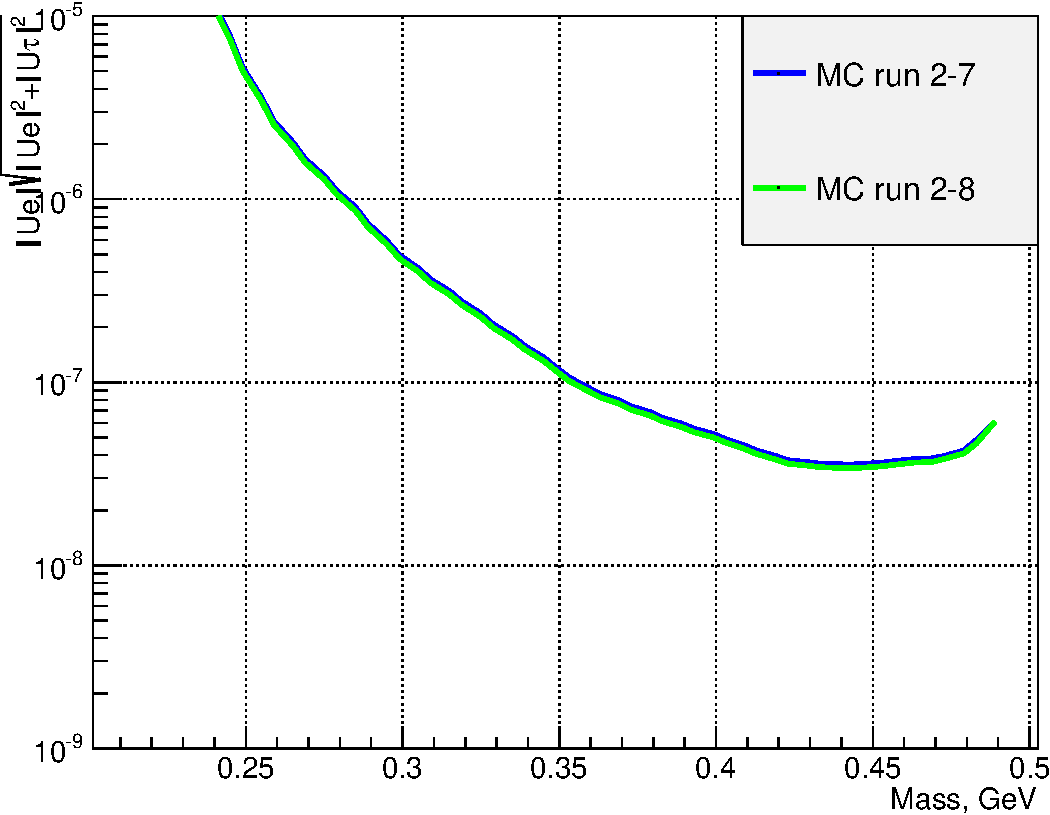
\includegraphics[width=\linewidth]{UeMixfullMC}  \\  $K^+\to e(\mu\mu\nu)$}
  \end{minipage}
  \caption{Sensitivity to mixing elements $\left|UeU\mu\right|$ and $\left|U_{e}\right|\sqrt{\left|U_{e}\right|^2+\left|U_{\tau}\right|^2}$ based on MC samples analysis.}
  \label{fig:HNL:LimitsMC2}
  \end{center}
\end{figure}

As one can see the improvements of PS191 limits can be obtained with the current statistics.

\section{Data unblinding}
\end{comment}

The numbers of observed events in data after the unblinding are presented in the \autoref{tbl:HNL:Ndata}. All the results are presented for the full ND280 data set (run 2-8).

\begin{table}[!ht]
\begin{center}
\begin{tabular}{llll}
                            & Events in data      \\
  $\mu\pi$ \hspace{0.5cm}   & 0  \hspace{2cm}     \\
  $e\pi$                    & 0                   \\
  $\mu\mu\nu$               & 1                   \\
\end{tabular}
\caption{The total number of events observed in data.}
\label{tbl:HNL:Ndata}
\end{center}
\end{table}

One event for the $N\to\mu\mu\nu$ mode was observed. It happened in the TPC3 and looks like a signal event: two muon-like tracks with the direction extremely collinear to the beam axis. The event display for this event is presented in \autoref{fig:HNL:DataEvent}.

\begin{figure}[!ht]
    \begin{center}
  \begin{minipage}{0.49\linewidth}
    \centering{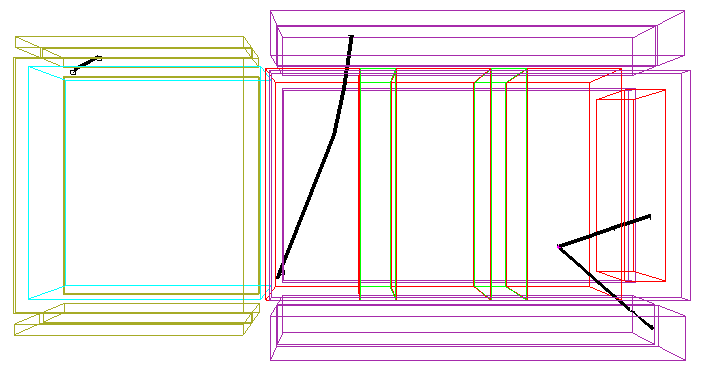
\includegraphics[width=\linewidth]{DataEvent2}}
  \end{minipage}
  \begin{minipage}{0.49\linewidth}
    \centering{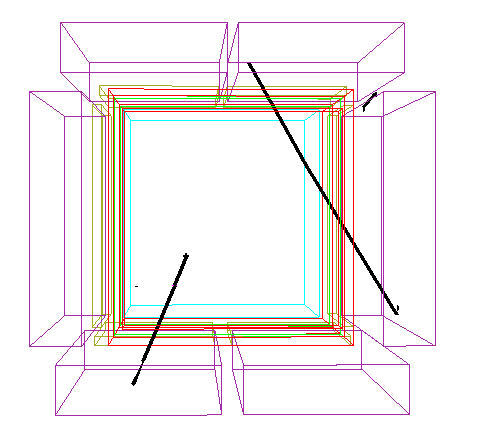
\includegraphics[width=\linewidth]{DataEvent1}}
  \end{minipage}
  \caption{Event observed in the $N\to\mu\mu\nu$ mode in the data sample in the TPC3.}
  \label{fig:HNL:DataEvent}
  \end{center}
\end{figure}

A more accurate study shows that the invariant mass of this muon pair is too high for the heavy neutrino decay $M_{inv}\approx$ GeV. But based on the blind analysis method and our analysis strategy this event will be treated as a signal and an appropriate upper limit on the mixing element will be set.

Based on these numbers final limits on the mixing elements based on our analysis can be set. The results are presented in \autoref{fig:HNL:LimitsData1} and \autoref{fig:HNL:LimitsData2}. The data statistics $\left(10.23\nu+6.29\bar{\nu}\right)\cdot 10^{20}POT$ was used.

\begin{figure}[!ht]
    \begin{center}
  \begin{minipage}{0.49\linewidth}
    \centering{\includegraphics[width=\linewidth]{Ue2fullDATA}  \\  $K^+\to e(e\pi)$}
  \end{minipage}
  \hfill
  \begin{minipage}{0.49\linewidth}
    \centering{\includegraphics[width=\linewidth]{Umu2fullDATA}  \\  $K^+\to \mu(\mu\pi)$}
  \end{minipage}
  \caption{Limits on mixing elements $\left|Ue\right|^2, \left|U\mu\right|^2$ based on the data samples analysis.}
  \label{fig:HNL:LimitsData1}
    \end{center}
\end{figure}

\begin{figure}[!ht]
    \begin{center}
  \begin{minipage}{0.49\linewidth}
    \centering{\includegraphics[width=\linewidth]{UeUmufullDATA}  \\  $K^+\to \mu(e\pi)$ and $K^+\to e(\mu\pi)$}
  \end{minipage}
  \begin{minipage}{0.49\linewidth}
    \centering{\includegraphics[width=\linewidth]{UeMixfullDATA}  \\  $K^+\to e(\mu\mu\nu)$}
  \end{minipage}
  \caption{Limits on mixing elements $\left|UeU\mu\right|$ and $\left|U_{e}\right|\sqrt{\left|U_{e}\right|^2+\left|U_{\tau}\right|^2}$ based on the data samples analysis.}
  \label{fig:HNL:LimitsData2}
  \end{center}
\end{figure}

\subsection{Prospects}
\label{sec:HNL:prosp}
The current study puts a conservative limit on the mixing elements of the heavy neutrino. A more accurate result can be obtained with precise background estimations. This work was continued by other collaborators and other methods were used for the data treatment. The accurate background estimations were developed and a new Markov Chain Monte Carlo method was used for the mixing elements limitation. All the production and decay modes of the heavy neutrino are analyzed together and a robust final result is obtained. The joint analysis including all the methods was published~\cite{Abe2019l}.

The T2K experiment will continue taking data. The preliminary plan is to accumulate $20\times10^{21}$ POT~\cite{Abe2016e}. With larger statistics (x11 to current) we will be more sensitive to the HNL mixing elements. Since the result is proportional to the square root from the expected events number the limits can be improved by the factor of 3.

The upgrade of the near detector complex is ongoing now~\cite{Abe2019} (also \autoref{pt:up}). Two additional TPCs will be installed. For the current study, it means that the fiducial volume will be extended by $\approx$10\%. That will also slightly improve the final result.

\end{document}